\documentclass[11pt,a4paper,british]{report}


\usepackage[backend=biber,mincitenames=1,maxcitenames=1,maxbibnames=99]{biblatex}
\bibliography{main}

% For full inline citing as used in the Related Publications section
% Thanks: https://tex.stackexchange.com/a/267089
\newcommand{\printpublication}[1]{\AtNextCite{\defcounter{maxnames}{99}}\fullcite{#1}}

\usepackage[dvipsnames]{xcolor}
\usepackage{graphicx}
\usepackage[hidelinks]{hyperref} 
\usepackage{listings}

\usepackage{booktabs}
\usepackage[style=Plaintop]{floatrow}
\usepackage[referable]{threeparttablex}

\usepackage{tkz-kiviat}
\usetikzlibrary{arrows}

\usepackage{setspace}
\setstretch{1.3}



\begin{document}



\begin{titlepage}
  \centering

  {\LARGE
    %Master's Thesis:\\
    A Comparative Study of Hadoop MapReduce,\\
    Apache Spark \& Apache Flink for Data Science
  \par}

  \vspace{2cm}

  {\large
    Bilal Akil\\
    Supervised by: A/Prof. Uwe R\"ohm\\
    ~\\
    Faculty of Engineering and IT\\
    School of Information Technology\\
    The University of Sydney, Australia\\
    {\tt bilal.akil@sydney.edu.au}
  \par}

  \vfill

  {\large\it
    A thesis submitted in fulfilment of the requirements\\
    for the degree of Master of Philosophy
  \par}

  \vspace{2cm}

  {\large March 2018 \par}
\end{titlepage}


\pagenumbering{roman}

{

  {\it
    I'll take this opportunity to express my deepest gratitude to Joy, my family, and Uwe R{\"o}hm, for your support and faith in my ability to persevere through this candidature. Without such, I surely would not have made it.

    Furthermore, I'd like to thank Uwe R{\"o}hm again, and Ying Zhou, Alan Fekete, and the school's Database Research Group, for the critical feedback and tutelage that kept this research on track and helped me to present at an international conference -- a feat I was doubtful of being able to achieve.
    
    I also acknowledge and appreciate the quality research of \citeauthor{VEIGA:EVALUATION:2015} \cite{VEIGA:EVALUATION:2015}, whose performance comparison data was used to accommodate the performance dimension of this multidimensional comparison. This has been further acknowledged within the thesis text wherever their research has been utilised.
  }

  Ying Zhou provided great assistance in updating the cluster and software for the usability study, as well as the Flickr data, problems, and solutions for assignment~1.
  
  Uwe R{\"o}hm, the supervisor for my Master's candidature, developed new, and updated existing learning materials for the course, which were depended on by the usability study, and helped immensely through all stages of its execution.
  
  They both provided invaluable feedback and support as I devised the usability study and compiled its results, as well as in reviewing and editing my writing of the below publications.


  \newpage
  \subsection*{Related Publications}

  The following publications arose from work related to this thesis, including some content from the introduction and conclusion, as well as from Chapters~2 and~3:
  
  \begin{itemize}
    \item \printpublication{AKIL:USABILITY:2017}
    \item \printpublication{AKIL:USABILITY_TR:2018}
  \end{itemize}
  

  \subsection*{Statement of Originality}

  This is to certify that to the best of my knowledge, the content of this thesis is my own work. This thesis has not been submitted for any degree or other purposes.

  I certify that the intellectual content of this thesis is the product of my own work and that all the assistance received in preparing this thesis and sources have been acknowledged.

  ~
  
  ~

  Bilal Akil
  

  \subsection*{Human Ethics}

  Ethics approval was attained prior to commencement of the usability study described in Chapter~3, from the University of Sydney's Human Research Ethics Committee under project number 2017/212. This application was supported by the university's Research Cluster for Human-centred Technology.

}

\newpage


\begin{abstract}
\thispagestyle{plain}
\setcounter{page}{3}

Distributed data processing platforms for cloud computing are important tools for large-scale data analytics. Apache Hadoop MapReduce has become the de facto standard in this space, though its programming interface is relatively low-level, requiring many implementation steps even for simple analysis tasks. This has led to the development of advanced dataflow oriented platforms, most prominently Apache Spark and Apache Flink. Those not only aim to improve performance, but also provide high-level data processing functionality, such as filtering and join operators, which should make data analysis tasks easier to develop. But with limited comparison data, how would data scientists know which system they should choose?

This research compares: Apache Hadoop MapReduce; Apache Spark; and Apache Flink, from the perspectives of performance, usability and practicality, for batch-oriented data analytics. We propose and apply a methodology which guides the preparation of multidimensional software comparisons and the presentation of their results. The methodology was effective, providing direction and structure to the comparison, and should serve as helpful for future comparisons. The comparison results confirm that Spark and Flink are superior to Hadoop MapReduce in performance and usability. Spark and Flink were similar in all three perspectives, however as per the methodology, readers have the flexibility to adjust weightings to their needs, which could differentiate them on a case-by-case basis.
  
We also report on the design, execution and results of a large-scale usability study with a cohort of masters students, who learn and work with all three platforms, solving different use cases in data science contexts. Our findings show that Spark and Flink are preferred platforms over MapReduce. Among participants, there was no significant difference in perceived preference or development time between both Spark and Flink. These results were included in the usability component of the multidimensional comparison. 

\end{abstract}





\setcounter{page}{4}
\tableofcontents


\chapter{Introduction}
\label{INTRODUCTION}
\pagenumbering{arabic}

  Across many scientific disciplines, automated scientific experiments have facilitated the gathering of unprecedented volumes of data, well into the terabyte and petabyte scale \cite{HeyTT:2009}. Big data analytics is becoming an important tool in these disciplines, and consequently more and more non-computer scientists require access to scalable distributed computing platforms. However, distributed data processing is a difficult task requiring specialised knowledge.

  Distributed computing platforms were created to abstract away distribution challenges. One of the most popular systems is Apache Hadoop which provides a distributed file system, resource negotiator, scalable programming environment named MapReduce, and other features to enable or simplify distributed computing \cite{HADOOP:HOMEPAGE,DeanG:MAPREDUCE:OSDI2004}. While a tremendous step in the right direction, effective use of this environment still requires familiarity with the functional programming paradigm and with a relatively low-level programming interface.
 
  Following the success of Hadoop MapReduce, several newer systems were created introducing higher levels of abstraction. MapReduce addresses the main challenges of parallelising distributed computations -- including high scalability, built-in redundancy, and fail safety. Newer systems including Apache Flink \cite{FLINK:HOMEPAGE,CarboneKEMHT:DEBU2015} and Apache Spark \cite{SPARK:HOMEPAGE,ZahariaCFSS:HotCloud10} extend their focus to the needs of efficient distributed data processing: dataflow control (including support for iterative processing), efficient data caching, and declarative data processing operators.

  Scientists have now a choice between several distributed computing platforms, and to guide their decision several comparison studies have been published recently \cite{BERTONI:EVAL_CLOUD_FRAMEWORKS:2015,MARCU:SPARK_VS_FLINK:2016,MEHTA:COMP_EVAL_BIGDATA_SYS:2017}. The focus of those studies was performance, which is perhaps not the primary problem for platforms built from the ground up with scalability in mind. More interesting is the question of the usability of those platforms, given that they will be used by non-computer scientists. Here we define usability as the ease of learning the concepts and usage of, and becoming proficient with a given system. But there are no reliable comparisons or large-scale usability studies so far.
  
  Furthermore, users would need to consider the practicality of the systems given their individual circumstances. For instance, is their existing cluster configuration supported by the system, and could they use a programming language for which they have already got a workflow and development environment setup? These real-world considerations are often left behind in system comparisons, but would be an important part of the decision making process for a potential user. The user may not have the know-how, or even permission, to enact changes on cluster configurations or install and configure new programming languages and environments.
  
  We have now described three factors that potential users tend to consider before deciding on a system to use: performance; usability; and practicality. While some may have the resources available to investigate these factors themselves, this will not be an option for many, who for the lack of other options, will instead resort to utilising software as described in previous research.
  
  This is often not a bad choice. However, it could sometimes lead to the usage of an inappropriate system, in turn increasing cost or reducing potential impact, for instance where a more appropriate system could have been used to run more experiments given the same amount of time and resources. In more extreme cases however, where too small a portion of research is conducted utilising modern or experimental technology in a particular discipline, it can be considered as slowing the technological progression of that discipline as a whole. As an example, we observed that when distributed computing is used in the bioinformatics discipline, MapReduce remains the dominant computational engine, which is strange considering both the performance and usability benefits of MapReduce's modern competitors -- see Chapter~\ref{SYSTEMS} Section~\ref{INTERDISCIPLINARY_USAGE} for this discussion. This could indeed be due to the repeated following of past practices, as the more modern options remain largely unexplored there.
  
  Thus we aim to provide a succinct, reliable multidimensional comparison of distributed computing engines that will help data scientists identify the system which would best suit their research, instead of potentially resorting to suboptimal tooling which could increase their effort and reduce their reward. The comparison must be suitable for viewers of differing technical backgrounds, as a data scientist or bioinformatician, for instance, would likely not be as familiar with the deeper concepts of distributed computing than a computer scientist would. And while all this will be useful in the present, the distributed computing space will continue to evolve, and these comparisons would need to be adjusted and repeated considering the major systems of the times, helping disciplines who utilise these tools to not fall behind -- which is similarly the case in contexts other distributed computing and data science, as the rapid development of technology is a somewhat universal challenge across both sciences and in the industry.
  
  To address these needs we propose a methodology for conceiving and displaying the results of multidimensional software comparisons, and employ it for the first time in this thesis. We present a comparison of Apache Hadoop MapReduce; Apache Spark; and Apache Flink, considering performance, usability and practicality, in a batch-oriented data analytics context. The performance component of the methodology will utilise an existing performance comparison (\citeauthor{VEIGA:EVALUATION:2015} \cite{VEIGA:EVALUATION:2015}) between the three systems; the practicality component consists of various static analyses; and to complete the usability component we combine static analysis with the results of a large-scale usability study that we performed as part of this thesis.
  
  The usability study was conducted within a cloud computing course at The University of Sydney. The course was targeted at masters students from various backgrounds, including IT and data science. It is, to the best of our knowledge, the largest usability study of modern data processing platforms. Participants of the study had to implement three different data analysis tasks with use cases involving social media, immunology and genomics. The first task was implemented using MapReduce, while the last two tasks were implemented in a crossed A/B test with half the class first using Flink and the other half Spark.
  
  All in all, this thesis details the following contributions:
  
  \begin{description}
    \item [Chapter~\ref{LITERATURE_REVIEW}] A literature review of related works considering existing comparisons, usability studies, and comparison methodologies, all in the context of distributed computing systems or software in general.
    \item [Chapter~\ref{LITERATURE_REVIEW} Section~\ref{INTERDISCIPLINARY_USAGE}] A survey of the types of software developed for large-scale DNA analysis in recent research from the BMC Bioinformatics journal (as performed using a custom web scraper) and the IEEE BigData conference.
  	\item [Chapter~\ref{USABILITY_STUDY}] Details on the design, execution, data analysis method and results of what is, to the best of our knowledge, the largest usability study of modern data processing platforms. We find that in-class usability studies are very effective and surprisingly underutilised (at least in the computer science space), and believe that our learnings in execution will prove useful in guiding others, thus discussing the successes and challenges met throughout our experience.
    \item [Chapter~\ref{COMPARISON}] The initial proposal of a methodology to conceive and display the results of multidimensional system comparisons, and its first application -- comparing Apache Hadoop MapReduce, Apache Spark and Apache Flink, from the perspectives of performance, usability and practicality, in a batch-oriented data analytics context.
  \end{description}

  Further in this chapter, you will find:
  
  \begin{description}
    \item [Section~\ref{STUDY_CONCEPTION}] The background of what led to this research, and its initial focus on bioinformatics.
    \item [Chapter~\ref{SYSTEMS}] Descriptions of the architecture and usage patterns of the compared systems.
  \end{description}
  

\section{Study Conception}
\label{STUDY_CONCEPTION}

  This research was originally focused on the bioinformatics discipline, where we heard from colleagues that new research was being conducted using Apache Hadoop MapReduce. With our knowledge of various modern distributed computing engines and the benefits they had, especially in terms of usability, we found it strange that Hadoop MapReduce was still being considered and used in new research.
  
  Looking further in to it, we got the impression that very little bioinformatics research was being conducted with MapReduce's modern descendants. Thus our initial project was to try and develop a better understanding of why this was the case (without going into the psychology or sociology of it), which involved exploring the strengths and weaknesses that the modern systems have in bioinformatics contexts. We found that the strengths did indeed outweigh the weaknesses, and so proceeded to investigate methods to increase awareness and adoption of these systems, with the goal of helping to lower their barriers to entry.
  
  Moving forward, we first performed a preliminary literature review and then a more thorough examination of recent bioinformatics research in an attempt to validate our intuition -- that the more modern systems were in fact being underutilised. The examination is presented in Chapter~\ref{SYSTEMS} Section~\ref{INTERDISCIPLINARY_USAGE} of this thesis, including details on the custom web scraper that was made to traverse, scrape and filter articles from the BMC Bioinformatics journal.
  
  Thus validated, we considered that a reliable, multidimensional system comparison in a bioinformatics context would serve as effective, and decided that this would become our goal. We then selected prominent distributed computing engines -- Apache Hadoop MapReduce; Apache Spark; and Apache Flink -- and worked to identify bioinformatics algorithms or tasks which both involve significant amounts of data, and present a variety of challenges in implementation or scalability. From that point we planned to implement each of the decided algorithms on each of the selected systems, thus providing the data for a comparison of the systems in terms of usability, performance, and the development experience as a whole.
  
  However before getting started with the implementations, we realised that there had to be more structure in the comparison and implementations such to reduce potential biases and increase the comparison's integrity. The first decision made was that instead of proceeding immediately to implementing an algorithm on each system, we should instead initially create a `blueprint implementation' for each task in an unrelated, non-distributed environment, such as plain Python, and then work on mapping that blueprint implementation to each of the individual systems. This would separate any difficulties in understanding and implementing the algorithm itself from struggles with the distributed computing systems.
  
  Secondly, some details for the comparison needed to be decided up front so we would know what to keep track of or look out for during the implementation process. It was this hurdle that led to the proposal of the methodology that will be discussed in Chapter~\ref{COMPARISON}. We realised the proposed methodology would need to be flexible enough to handle the different use cases and systems, and with a bigger picture in mind, also different comparison dimensions and audiences -- otherwise there would be little benefit in proposing a methodology at all.

  Following completion of the first blueprint, where the use case was DNA short-read correction based on the Blue algorithm \cite{GREENFIELD:BLUE:2014}, we presented our project and an early draft of the methodology to The University of Sydney's Database Research Group, of which we were members of, and received important feedback which resulted in our research changing direction towards what it is now. The group emphasised that while the methodology is conceptually sound, the usability component of the comparison would suffer greatly from the subjectivity in having a single person (myself) implement the use cases across the systems -- especially considering that we are not members of the target audience.
  
  Instead they strongly suggested performing a usability study, and fortunately we had the opportunity to do so. Thus the direction of the research changed: with a cloud computing course starting in the coming months, we switched focus to attaining ethics approval and developing a usability study to be run as part of that class. The design, execution, data analysis method and results of the usability study are discussed in Chapter~\ref{USABILITY_STUDY}. Data from the usability study corresponded with the usability component of the comparison, alongside some additional static analyses. The performance component was covered using existing research between the systems, of which we found plenty to exist, and `static' research was performed to complete the practicality component by examining the characteristics of each system.
  
  
\section{Systems}
\label{SYSTEMS}

  Apache Hadoop MapReduce \cite{DeanG:MAPREDUCE:OSDI2004} has long been the de facto standard for large-scale data analytics, being one of the earliest systems available to abstract the challenges of distributed computing and fault tolerance away from its users, significantly reducing the barrier to entry that was present in the big data space.

  Its success led to the creation of systems which provided higher-level approaches to distributed computing. Apache Spark \cite{ZahariaCFSS:HotCloud10} and Apache Flink (formerly Stratosphere) \cite{CarboneKEMHT:DEBU2015} are two prominent examples of such systems. Spark and Flink are seen as common rivals, and have had much attention paid to their performance merits and pitfalls \cite{MARCU:SPARK_VS_FLINK:2016,PereraPH:CORR2016,VEIGA:EVALUATION:2015}. However, these comparisons focus primarily on the systems' performance, while this comparison is also to consider usability and practicality.

  Due to their prominence and competitiveness, Spark and Flink will be the subject of this study's comparison. Hadoop MapReduce will also be part of the comparison, acting more as a control of sorts, allowing examination of the relative advantages or disadvantages of each newer system compared. We examined data from Google Scholar, the IEEE BigData Conference and the BMC Bioinformatics journal, in an attempt to confirm that MapReduce did indeed remain the dominant choice for distributed computing in bioinformatics and likely other scientific disciplines, as discussed in this chapter's interdisciplinary usage section. 

  For the purpose of the usability study in Chapter~\ref{USABILITY_STUDY}, all three systems were run using Apache Hadoop YARN for resource management \cite{VAVILAPALLI:YARN:2013} and HDFS as the distributed file system \cite{SHVACHKO:HDFS:2010}. The following versions were used in the usability study: Apache Hadoop MapReduce v2.7.2; Apache Spark v2.1.1; Apache Flink v1.2.1. These were all the stable or highest non-beta versions at the time of the study's preparation.
  
  The three following sections will describe the background and architecture of each system, as well as a high-level description of their usage. Then Section~\ref{INTERDISCIPLINARY_USAGE} will discuss the apparent prevalence of each system in scientific disciplines like bioinformatics.


\subsection{Apache Hadoop MapReduce}

  This brief history of Apache Hadoop is paraphrased and summarised from an enjoyable article by \citeauthor{BONACI:HADOOP_HISTORY:2015} \cite{BONACI:HADOOP_HISTORY:2015}.
  
  Hadoop has a long history, having been given a name by Doug Cutting in 2006 but in development much earlier. Cutting was working with Mike Cafarella from the University of Washington with the aim of indexing the entire web, and also running Google's PageRank algorithm against it. Of course this proved an immense challenge in distribution and scalability -- hence the creation of Hadoop's HDFS, MapReduce, and then YARN and MapReduce 2. The former two were born with inspiration from Google publications including The Google File System \cite{ghemawat2003google} and MapReduce \cite{DeanG:MAPREDUCE:OSDI2004}.
  
  Following Hadoop's initial success at Google, Yahoo! took guidance from Cutting to get themselves on-board with Hadoop, which proved to be a great decision for the company. Later, newer web-scale companies like Twitter, Facebook and LinkedIn started using Hadoop and contribute to its open source codebase and tooling, thus continuing to grow the software's ecosystem. In 2008 Hadoop transitioned from a subproject of Apache Lucene to the top level Apache Hadoop where it still remains, now with many subprojects of its own.

  A large part of its success was due to how it abstracted away many distributed computing challenges from its users, being one of the earliest systems to do so. HDFS was presented as a single reliable file system, when in fact it handled the tasks of monitoring for failures and rebalancing the distribution of blocks, while itself not imposing any restrictions on schema or structure. Its acceptance of failure promoted a shift from expensive, specialised hardware to commodity hardware: if your scale is large enough, there are inevitably going to be hardware failures, so why not expect them instead of treating them as an exception? MapReduce further solved the problems of parallelisation, distribution and fault tolerance in program execution. 

  However, the original MapReduce had a flaw in the sense that it practically handled all responsibilities (other than the distributed file system), including scheduling, managing job execution, interfacing towards clients, and of course actually executing the provided code and managing the flow of data. As a growing number of specialised applications requiring different processing models demanded attention, newer distributed computing engines to support them had to either be build atop MapReduce itself, or face the challenge of reimplementing the surrounding tooling like scheduling and managing job execution. This was a problem because MapReduce's batch processing model is not suitable for all applications, being especially problematic for those requiring iterative execution like machine learning or graph processing.

  Thus YARN (Yet Another Resource Negotiator) was born, separating the resource management, workflow management and fault-tolerance from MapReduce, and allowing other frameworks to be built atop it. MapReduce was modified to use YARN, becoming MapReduce 2.


\subsubsection{Usage}

  As the name suggests, Apache Hadoop MapReduce is executed in the Hadoop ecosystem, typically utilising YARN for cluster management \cite{VAVILAPALLI:YARN:2013} and HDFS as a distributed file system \cite{SHVACHKO:HDFS:2010}. Specifically, Hadoop MapReduce is a software framework which is managed by Hadoop YARN, a resource negotiator. HDFS is separate in the sense that it does not run on YARN, however the software is distributed as a part of the Hadoop ecosystem.
  
  MapReduce jobs usually utilise HDFS for input and output, often on the same nodes to minimise data transportation. MapReduce communicates with YARN for resource negoitation and scheduling, and monitors the running jobs in case it needs to request re-execution from YARN.
  
  The architecture of YARN and HDFS will not be described here, as they are shared between the comparison of the three distributed computing systems. You can learn more about YARN and HDFS from the Hadoop website \cite{HADOOP:HOMEPAGE}, which provides great descriptions of their architectures.

  MapReduce facilitates the fault-tolerant, distributed execution of `jobs' or applications, which encompasses the following processing steps:
  
  \begin{enumerate}
    \item Read input from HDFS blocks and split to mappers.
    \item Map, applying a user-defined function (UDF) in a completely parallel manner.
    \item If there is no reducer specified: output one file per mapper, typically to HDFS, and finish.
    \item Optionally combine output from mappers using a UDF.
    \item Partition, shuffle, sort and merge data into reducers. Default partition and sort behaviour can be overridden.
    \item Reduce using a UDF, turning multiple values per key into a single value, also in a completely parallel manner (per key).
    \item Output one file per reducer, typically to HDFS.
  \end{enumerate}
  
  In MapReduce, the user provides a driver Java class which utilises the MapReduce package to configure, start and interact with jobs. It can access written data between jobs by reading their output, for instance from HDFS.
  
  Alternatively, in streaming mode, the driver is instead a set of shell commands, where scripts are specified to act as the mapper, combiner and reducer, each operating via standard input and output. This allows any method of programming available throughout the cluster to be used, and may present other contextual advantages or disadvantages \cite{DING:HADOOP_STREAMING:2013}. Chaining jobs would then become a matter of chaining shell commands.
  
  The mapper and reducer are classes or scripts that operate on key value pairs. A single mapper receives an iterator of key value pairs and can output zero or more key value pairs. A single reducer receives one key and an iterator of values -- or an iterator of key value pairs in sorted key order in Hadoop Streaming -- and can output zero or more key value pairs. A combiner is a reducer that is executed on each mapper following mapping but prior to data being shuffled over the network, primarily used to reduce communication overhead.
  
  Other distributed computing operations are implemented in terms of mapping and reducing. For instance, filter is usually performed in the map step, while joining and aggregation would be in one or both of the mapper and reducer, presenting different trade-offs \cite{BLANAS:MR_JOINS:2010}. Iteration can be implemented using a loop in the driver, and in that loop configuring and starting new jobs that use the previous completed jobs' output. Higher level systems have been created to improve support for or simplify iteration in MapReduce, such as Twister \cite{EKANAYAKE:TWISTER:2010}.


\subsection{Apache Spark}

  Spark was born in 2012 by the need for improvement for iteration and data mining algorithms, with its initial publication of Resilient Distributed Datasets (RDDs) which ``lets programmers perform in-memory computations on large clusters in a fault-tolerant manner'' \cite{ZAHARIA:RDD:2012}.

  Soon after, \citeauthor{ZAHARIA:DSTREAM:2012} announced Discretized Streams, providing a ``high-level programming API, strong consistency, and efficient fault recovery'' to distributed stream computation, in the Spark environment. Thus Spark became one of the earliest high-level systems supporting both distributed batch and stream computation, as well as iterative querying.

  Its high-level API was a breath of fresh air compared to the verbosity of Apache Hadoop MapReduce, and while initially available in Scala, its APIs soon became available in Java and Python, and later R.

  Open source at its inception, the project was later donated to the Apache Foundation, whence it became the top level Apache Spark in 2014. By then the project already had a significant contributor and user base, which continued to grow to today's staggering levels -- considerably Hadoop MapReduce's top competitor, as explored in Section~\ref{INTERDISCIPLINARY_USAGE}.


\subsubsection{Usage}
  
  \begin{lstlisting}[float=ht,
                     language=Python,
                     basicstyle=\ttfamily\footnotesize,
                     label=SPARK_WORDCOUNT,
                     caption={Apache Spark Python word count example as shown at: \url{https://spark.apache.org/examples.html}}]

text_file = sc.textFile("hdfs://...")
counts = text_file.flatMap(lambda line: line.split(" ")) \
             .map(lambda word: (word, 1)) \
             .reduceByKey(lambda a, b: a + b)
counts.saveAsTextFile("hdfs://...")
  \end{lstlisting}
  
  Apache Spark turns input data into RDDs, and then applies lazy transformations to them, creating new RDDs, where execution of said transformations do not occur until necessary for consumption by an `action' -- for instance for collection onto the driver or for storage into HDFS.

  Spark has resource requests fulfilled by one of three resource managers: Spark Standalone; YARN; or Apache Mesos. Its core API features various generic transformations and actions, and additional APIs have been built atop the core API to provide higher-level support for various contexts. API libraries are provided for different programming languages, with the core API currently supporting Scala, Java, Python and R.
  
  The driver is any program which utilises the core API and optionally the other more specialised APIs. It creates RDDs from various input sources, including the local file system or HDFS, and applies lazy transformations and actions to those RDDs. The driver can also be an interpreter, which is often useful for exploration or debugging.
  
  Iteration can be performed similarly to Apache Hadoop MapReduce; using a loop in the driver. However, instead of configuring, starting and blocking on new jobs which write to and from HDFS, Spark would simply apply additional lazy transformations, collect them into a variable when necessary, and repeat.
  
  Spark predominantly performs in-memory computation in an attempt to minimise disk communication. This has the potential to provide speed improvements compared to MapReduce in many situations, including iteration, but can also degrade performance if memory is insufficient \cite{GU:MEM_OR_TIME:2013}. More effort is being dedicated to improving memory management to improve resiliency and performance \cite{MARCU:SPARK_VS_FLINK:2016}.
  
  The core API operates on either key value pairs or arbitrary objects. It includes transformations such as: \texttt{map}, \texttt{filter}, \texttt{reduceByKey}, \texttt{distinct}, \texttt{union}, \texttt{intersection}, \texttt{sortByKey}, \texttt{aggregateByKey}, \texttt{join}, and so forth. Actions include \texttt{saveAsTextFile}, \texttt{collect}, \texttt{count}, \texttt{countByKey}, \texttt{first}, \texttt{foreach}, \texttt{takeSample}, and so forth. Some transformations or operations can only operate on key value pairs -- not on arbitrary objects.
  
  With thanks to its high-level APIs, Apache Spark programs can end up looking quite simple, such as in the word count example in Listing~\ref{SPARK_WORDCOUNT}. However, in reality users will need to understand various system internals, such as when data is shuffled, to support the design of efficient and scalable programs.
  
  Fault tolerant, distributed stream processing is achieved in Apache Spark by using the Spark Streaming extension of the core API. It works by dividing or `micro-batching' live input data streams into a `discretized stream' or \texttt{DStream} \cite{ZAHARIA:DSTREAM:2012}, which is a sequence of RDDs that can be operated on by the core API and with additional streaming operations such as \texttt{window}. Other Spark API libraries, including MLlib and GraphX, also provide \texttt{DStream} support. Spark's method of micro-batching has been found to be slower, but more resilient to failure than native streaming in Apache Storm and Apache Flink \cite{LOPEZ:STREAM_COMPARISON:2016}.

  Spark's core APIs have been revamped in more recent versions. Looking at the documentation for Spark v2.2.1 -- the stable version at the time of performing the comparison in Chapter~\ref{COMPARISON} -- we can see that usage of \texttt{DataSet} and \texttt{DataFrame} APIs are recommended for working with RDDs, or Spark SQL for relational data.
  

\subsection{Apache Flink}

  In 2014, \citeauthor{ALEXANDROV:STRATOSPHERE:2014} presented Stratosphere \cite{ALEXANDROV:STRATOSPHERE:2014}, an ``open-source software stack for parallel data analysis'' which included a program optimiser, and at the time its own query language named Meteor, and much more. It claimed a major point of differentiation from competing systems was in its support for efficient incremental iteration. 

  In one year's time the engine received a great amount of attention and development. While it maintained most of its architectural and conceptual features, much of its implementation changed, and even its name changed as it become the top level Apache Flink \cite{CarboneKEMHT:DEBU2015}.

  For instance, the Meteor query language was no longer mentioned. Instead, Flink featured a \texttt{DataSet} API for batch processing, and a \texttt{DataStream} API for stream processing, which would both execute against a `common fabric' of streaming dataflows.

  Thus was one of Flink's highlights: the unification of stream and batch processing. In fact, Flink treated a batch process as a special case of a stream process -- where the stream is finite. Furthermore, the project boasted a strong, wide set of features, supporting incremental asynchronous stream iterations, query optimisation, its own memory management to support spilling to disk in memory intensive applications, and more.


\subsubsection{Usage}
  
  Apache Flink has changed much since its Stratosphere days. Thus, the information here is based on the Apache Flink v1.2 documentation found at \url{https://flink.apache.org}.
  
  Flink is natively a stream processor where batch processing is represented as a special case of steaming -- more specifically, bounded streaming with some adjustments to features such as fault tolerance and iteration. In Flink, users specify lazy streams and transformations which the engine then maps to a streaming dataflow using a cost-based optimiser. This dataflow is a directed acyclic graph (DAG) from sources to sinks, with transformation operators in between. Sinks trigger the execution of necessary lazy transformations.

  The engine can be run in standalone, Hadoop YARN, or Apache Mesos cluster modes, similar to Apache Spark. It provides APIs with different levels of abstraction. The core \texttt{DataSet} (batch) and \texttt{DataStream} APIs are the most commonly used, with table and SQL APIs sitting at atop them. Other libraries are provided to directly support various specific contexts. Core API libraries are provided for Java and Scala, with the \texttt{DataSet} API additionally supporting Python.
  
  Similar to Apache Spark, the driver is any program which utilises the Flink APIs. It creates \texttt{DataSet}s or \texttt{DataStream}s from various input sources and applies lazy transformations to them, creating new \texttt{DataSet}s or \texttt{DataStream}s, until eventually directing them all various sinks.
  
  Iteration can be achieved either using a loop in the driver, or via the \texttt{IterativeStream} or \texttt{IterativeDataSet} classes. Using a loop is technically not iteration, but rather the driver continuously extending the DAG as necessary, which is limited in its scalability. The provided classes, on the other hand, can be thought to add a single node in the DAG which performs a set of transformations iteratively (given exit conditions), either using the last computed value or a solution set state that is modifiable in each iteration.
  
  Flink also primarily utilises in-memory computation to minimise disk communication. For robustness it implements its own memory management within the JVM, attempting to reduce garbage collection pressure, prevent out of memory errors by spilling to disk, and more. 
  
  The system does not operate on key value pairs, but requires `virtual' keys for some operators like grouping. Instead, it operates on arbitrary data types, and provides additional support for tuples and `plain old Java objects' (POJOs) by simplifying keying -- allowing specification of `virtual' keys as a tuple index or object property.
  
  Its core API supports a set of transformations that is largely similar to those in Spark's core API. As a result, Flink programs can also appear quite simple upon completion, but its users also will need to understand various system internals, such as when data is shuffled, to support the design of efficient and scalable programs.
\chapter{Literature Review}
\label{LITERATURE_REVIEW}

  The first section of this literature review searches for related work comparing the subject distributed computing systems, considering performance and other factors. The second examines usability studies which compared programming systems and were set in university class contexts, and the third attempts to find existing methodologies or other relevant information on multidimensional software comparisons.


\section{System Comparisons}
\label{SYSTEM_COMPARISONS}

  There have been several comparison studies of distributed computing engines in the context of scientific applications before, which however typically focus on the performance and scalability of the systems, somewhat neglecting usability metrics. For example, \citeauthor{BERTONI:EVAL_CLOUD_FRAMEWORKS:2015} are comparing Apache Flink and Apache Spark with regard to genomics applications \cite{BERTONI:EVAL_CLOUD_FRAMEWORKS:2015}, but only report on differences in implementation techniques and runtime performance. Similar performance comparison studies of Spark and Flink with varying analytical workloads have been done by \citeauthor{MARCU:SPARK_VS_FLINK:2016} \cite{MARCU:SPARK_VS_FLINK:2016}, \citeauthor{PereraPH:CORR2016} \cite{PereraPH:CORR2016}, \citeauthor{VEIGA:EVALUATION:2015} \cite{VEIGA:EVALUATION:2015}, and likely others.
  
  We will in fact be utilising experimental results from the last mentioned paper by \citeauthor{VEIGA:EVALUATION:2015} \cite{VEIGA:EVALUATION:2015} to accommodate the performance component of our multidimensional comparison. This decision was made considering that this thesis involves performing a broad and comprehensive comparison of the systems -- not specific only to performance. Being a Master's candidature, and with effort needing to be devoted to the other aspects of the comparison and development of a methodology, we would not be able to perform as thorough and diligent a performance comparison as \citeauthor{VEIGA:EVALUATION:2015} have.
  
  We choose this research because it compares the same systems as ours, exercising the three systems against six tasks -- some characterised as CPU bound, one I/O bound, and three iterative algorithms -- on common big data benchmarks including as TeraSort, PageRank, and $k$-means. Careful attention was paid to the configuration of each system, and one section of the comparison was even devoted to the impact of parameter tuning. For the purpose of our research, we use their execution speed results in completing the six tasks, and also look at how the speed changes as the number of nodes used increases. The application of this paper's findings in our comparison can be found in Chapter~\ref{COMPARISON}.

  It is clear that plentiful research is available in regards to the performance of these distributed computing engines. However, there were far fewer options when it came to multidimensional comparisons, and especially comparisons focusing on non-performance related comparisons like usability or practicality.

  \begin{itemize}
    \item \citeauthor{MEHTA:COMP_EVAL_BIGDATA_SYS:2017} present a study comparing five big data processing systems (Apache Spark; SciDB; Myria; Dask; and TensorFlow) with regard to their suitability and performance for scientific image analysis workflows \cite{MEHTA:COMP_EVAL_BIGDATA_SYS:2017}. This paper also gives a brief qualitative assessment of each system, considering the ease of use and overall implementation complexity, however based on measuring lines of code and observing issues experienced during implementation -- not quite capturing the usability of the systems.
    \item \citeauthor{RICHTER:COMPARISON:2015} present a multidimensional comparison of Apache Hadoop MapReduce, Apache Storm and Spark via some of their higher level APIs, like MlLib for Spark, in the context of various distributed computing algorithms such as $k$-means and linear regression \cite{RICHTER:COMPARISON:2015}. The dimensions of the comparison include four performance or `capability' related metrics -- speed, fault tolerance, scalability and extensibility -- and also usability. However, the usability dimension appears to primarily be based on static analyses, for instance of the available interface features or programming language support, providing little information on the ease of use or human interaction aspect, and how the final scores were actually decided. This is yet another a good performance comparison, however lacking depth in the usability dimension.
    \item \citeauthor{GALILEE:COMPARISON:2014} present a poster comparing Hadoop MapReduce, Spark and Flink on the grounds of performance, understandability, usability and practicality \cite{GALILEE:COMPARISON:2014}. It is refreshing to see a focus on these non-performance related factors, however considering the nature of the publication, there is lacking detail in how the scores were compiled, and concern over the subjectivity in having been performed all from a single researcher's perspective.
  \end{itemize}

  We can see that performance comparisons are plentiful, and that what we have found will be sufficient in accommodating the performance aspect of our multidimensional comparison -- specifically by using the data from \citeauthor{VEIGA:EVALUATION:2015} \cite{VEIGA:EVALUATION:2015} which provides both the system coverage we require at a level of quality that consider reliable. Now we will shift focus to the important factors of usability and practicality, which was notably lacking in the above articles. Without this information available, potential users will find it difficult to accurately and efficiently judge the applicability of these systems to their use cases. This is especially a problem for users without a strong technical background, as they perhaps would not be able to compare and judge these factors themselves.


\section{Usability Studies}

  We found no usability studies comparing the exact set of distributed systems in this paper, or in fact any distributed systems at all. Thus we had to broaden our search in an attempt to learn what challenges laid ahead of us, and of any useful techniques that could improve the quality of our usability study. Particularly, we were looking for usability studies which compared two or more programming systems, and was set in a university class or course environment.
  
  The usability study by \citeauthor{NANZ:CONCURRENCY_STUDY:2013} \cite{NANZ:CONCURRENCY_STUDY:2013} compared concurrent programming languages, and while similar in how it subjected a university class to two different programming languages and compared the results, it had spanned only four hours and was set in a more controlled environment -- in that participants utilised self-study material under supervision, and continued to the measured exercise session later on the same day -- and thus would not face many of the challenges that our semester-long study would. With that being said, this research was excellently composed and executed, so despite it not being especially applicable to our situation as just described, it still contained helpful advice and techniques that we tried to implement in our study such to increase its reliability and reduce potential biases.
  
  The usability study by \citeauthor{HOCHSTEIN:CONCURRENCY_STUDY:2008} \cite{HOCHSTEIN:CONCURRENCY_STUDY:2008} compared the programming effort of two parallel programming models. While being roughly similar to the previous paper in terms of comparative nature and participant base, it had a time-frame of two weeks, which is notably closer to our intentions than the previous paper's four hours. However, this one heavily utilised instrumented compilers in producing its data, which in our case would be impractical considering time restraints and system complexity. It also was focused on comparing effort in the form of development time and correctness, which we felt would not be sufficient to describe and compare the broader usability of a system.
  
  In both of these studies, participants were grouped and only used one of the two compared systems, with data being compared across the groups. Our study differs in that participants would use each of the three systems and provide feedback on them all. This would present a series of challenges for us, such as dealing with potential first-used biases, which we unfortunately did not manage to find any guidance on via literature review.


\section{Comparison Methodologies}

  Our research aims to compare multiple systems, considering multiple dimensions, and faced the challenge of devising, collecting and portraying those results effectively. The display of the results must be suitable for audiences of differing technical ability. Before deciding to propose a comparison methodology that meets these requirements, we of course searched for any existing methodologies that could be used or learned from.

  Interestingly, none were found. The search was continually broadened, from being for multidimensional comparisons of software or programming systems, to multidimensional comparisons in any context, to comparison methodologies in general, and yet nothing relevant could be found.

  Comparisons do indeed need to be context appropriate in how they are performed and displayed, perhaps explaining the lack of a developed methodology. Particularly in regards to the display, there are many creative approaches that could be more suitable to given audiences, and so authors would likely do what seems best for them rather than using a standard methodology. For instance, it is common to see infographics used to display comparison results online -- to a non-technical audience -- but it is not always appropriate, and so would likely not be found in any particular methodology.
  
  With that being said, we still aim to apply a well-thought methodology to this thesis' comparison, and so have taken the step to propose one in Chapter~\ref{COMPARISON} considering the lack thereof. This methodology will be quite high-level or generalised, allowing it to guide researchers with different contexts or needs instead of only being useful in very similar circumstances to ours.



\section{Interdisciplinary Usage}
\label{INTERDISCIPLINARY_USAGE}

  \begin{table}[ht]
    \centering
    \setlength\tabcolsep{3pt}

    \caption{Google Scholar search results}
    \label{GSR}

    \makebox[\textwidth]{\begin{threeparttable}
      \scriptsize
      \begin{tabular}{l | l l l l}
        \toprule
        \textbf{Query}                                          & \textbf{2015/06/22} & \textbf{2016/04/26} & \textbf{2016/09/15} & \textbf{2018/01/30} \\
        \midrule
        ``hadoop'' dna alignment OR assembly OR searching       & 1220\tnotex{GSR:A}  & 1520\tnotex{GSR:A}  & 1740\tnotex{GSR:A}  & 2690\tnotex{GSR:A}  \\
        ``apache spark'' dna alignment OR assembly OR searching & 46\tnotex{GSR:A}    & 104\tnotex{GSR:A}   & 163\tnotex{GSR:A}   & 444\tnotex{GSR:A}   \\
        ``apache storm'' dna alignment OR assembly OR searching & -\tnotex{GSR:B}     & 18                  & 33\tnotex{GSR:A}    & 68\tnotex{GSR:A}    \\
        ``apache flink'' dna alignment OR assembly OR searching & 1                   & 9                   & 18\tnotex{GSR:A}    & 52\tnotex{GSR:A}    \\
        ``apache hama'' dna alignment OR assembly OR searching  & -\tnotex{GSR:B}     & 6                   & 8                   & 10                  \\
        ``apache apex'' dna alignment OR assembly OR searching  & -\tnotex{GSR:B}     & 0                   & 1                   & 2                   \\
        \bottomrule
      \end{tabular}
      \normalsize
      \begin{tablenotes}
        \item[a] \label{GSR:A} Result is approximate, indicated as ``About 46 results'' instead of ``46 results'' (for instance) on the search results page.
        \item[b] \label{GSR:B} That particular query was not performed at that time.
        \source \url{https://scholar.google.com/} -- The raw number of search results given a particular search query, with numbers collected at 2015/06/22, 2016/04/26, 2016/09/15 and 2018/01/30. Note that the query dates are not evenly separated.
      \end{tablenotes}
    \end{threeparttable}}
  \end{table}

  The hypothesis that led to us starting this research project was specific to the bioinformatics discipline -- that Apache Hadoop MapReduce remained the dominant distributed computing engine despite the recent development of more modern dataflow-oriented platforms such as Apache Spark or Apache Flink. We took some steps to validate this hypothesis on a larger scale by surveying the literature, however still within the context of bioinformatics.
  
  We believe that if the problem exists in the bioinformatics discipline, it would likely exist in other scientific disciplines where big data plays a similarly critical role, such as in astronomy, chemistry, and likely many other natural sciences. As these disciplines continue to collect significantly more data from significantly more numerous and powerful sensors, they face a similar challenge to bioinformatics, in that they grow increasingly reliant on distributed computing systems despite their practitioners often lacking the traditional computing background necessary to operate them without great difficulty.

  The intention in this section is to give an overview and to highlight any trends that may be present in the usage of distributed data science platforms, rather than to provide a fine-grained measurement of the system usage in each individual disciplines, which would be a very difficult task. Considering this, we concentrated on one specific application area of data science, namely bioinformatics.

  Our first attempt at gauging usage trends for each system, in the middle of 2015, was to compare the number of Google Scholar query results between each system, as portrayed in Table~\ref{GSR}. To this end, we issued several search queries to Google Scholar, each looking for the mentioning of a different data processing platform in the context of a research paper on DNA alignment, sequencing or searching. Indeed, this is not a precise measurement, as there would likely be many false-positives. However after cross-checking a sample of these papers (see below in Section \ref{SCRAPER}), we are positive that simply observing differences in the order of magnitude between the systems provides a good indication of an apparent trend. For instance, in the first measurement in June 2015 it was clear that Hadoop was almost the only compared system being compared at all, with Apache Spark only beginning to emerge with 3.77\% of Hadoop's occurrences.

  It is interesting to see that trend change over time, as other systems begin to emerge. However, they all remain mostly negligible in comparison to Hadoop and Spark, as the number of articles for both continue to grow, with Spark amounting to 16.51\% of Hadoop's occurrences by the beginning of 2018 -- a substantial improvement from 3.77\%, and almost seven times more than any other compared system.

  Thus this rough observation supports the hypothesis that Hadoop MapReduce remains the dominant choice, but by a shortening margin, with Spark particularly on the rise. The following subsections will attempt to provide more specific measurements to support this hypothesis.


\subsection{Web Scraper}
\label{SCRAPER}

  \begin{table}[ht]
    \centering
    \setlength\tabcolsep{3pt}

    \caption{BMC Bioinformatics system usage web scraper results}
    \label{SR:BMC}

    \makebox[\textwidth]{\begin{threeparttable}
      \scriptsize
      \begin{tabular}{l l l l}
        \toprule
        \textbf{DOI} & \textbf{Keywords} & \textbf{Suitable?} & \textbf{Software} \\
        \midrule
        10.1186/s12859-016-1179-2 & ('fasta',) & YES & Vaadin (Java), R \\
        10.1186/s12859-016-0904-1 & ('fastq', ' sam[ .,]') & YES & SparkSQL (mod.) \\
        10.1186/s12859-015-0812-9 & ('fasta', 'fastq', 'genbank', ' sam[ .,]') & YES & SAS, Perl \\
        10.1186/s12859-016-0915-y & ('fasta', 'fastq') & YES & Python2 \\
        10.1186/s12859-016-1014-9 & ('fasta', 'fastq', ' sam[ .,]') & YES & Python2 \\
        10.1186/s12859-015-0705-y & ('fasta', ' sam[ .,]') & YES & Python2 \\
        10.1186/s12859-016-0967-z & ('fastq',) & YES & Perl, R \\
        10.1186/s12859-015-0800-0 & ('fasta', 'fastq') & YES & Perl, R \\
        10.1186/s12859-016-0969-x & ('fasta',) & YES & Perl \\
        10.1186/s12859-016-1159-6 & ('fasta', 'fastq', 'genbank') & YES & MapReduce, C++, Ruby, ... \\
        10.1186/s12859-015-0744-4 & ('genbank',) & YES & CUDA \\
        10.1186/s12859-016-0887-y & ('fasta',) & YES & Celery, RabbitMQ, Django, ... \\
        10.1186/s12859-016-1069-7 & ('fastq',) & YES & C++ \\
        10.1186/s12859-015-0798-3 & ('fasta',) & YES & C, Java \\
        10.1186/s12859-016-0930-z & ('fasta', 'fastq') & YES & C \\
        10.1186/s12859-015-0736-4 & ('fastq', ' sam[ .,]') & YES & Unknown... \\
        10.1186/s12859-016-0881-4 & ('fasta', 'fastq', ' sam[ .,]') & TRANSCRIPTOME & \\
        10.1186/s12859-015-0698-6 & ('gcg',) & TRANSCRIPTOME & \\
        10.1186/s12859-015-0826-3 & ('fasta',) & SMALLSCALE & \\
        10.1186/s12859-016-1057-y & ('fasta',) & SMALLSCALE & \\
        10.1186/s12859-015-0785-8 & ('fasta',) & SMALLSCALE & \\
        10.1186/s12859-015-0711-0 & ('fasta',) & SMALLSCALE & \\
        10.1186/s12859-016-1146-y & ('fasta',) & SMALLSCALE & \\
        10.1186/s12859-015-0840-5 & ('fastq', 'genbank') & PIPELINE/PLATFORM & \\
        10.1186/s12859-015-0795-6 & ('fasta', 'fastq') & PIPELINE/PLATFORM & \\
        10.1186/s12859-016-1104-8 & ('fastq',) & PIPELINE/PLATFORM & \\
        10.1186/s12859-016-0892-1 & ('fasta', 'fastq') & PIPELINE/PLATFORM & \\
        10.1186/s12859-016-0879-y & ('fasta', 'fastq', ' sam[ .,]') & PIPELINE/PLATFORM & \\
        10.1186/s12859-015-0837-0 & ('fasta',) & PIPELINE/PLATFORM & \\
        10.1186/s12859-016-0966-0 & ('fasta', 'fastq') & PIPELINE/PLATFORM & \\
        10.1186/s12859-015-0726-6 & ('genbank', ' sam[ .,]') & NOTSOFTWARE & \\
        10.1186/s12859-015-0778-7 & ('fastq', ' sam[ .,]') & NOTSOFTWARE & \\
        10.1186/s12859-016-1052-3 & ('fastq',) & NOTSOFTWARE & \\
        10.1186/s12859-015-0709-7 & ('fasta', 'fastq') & NOTANALYSIS & \\
        10.1186/s12859-016-1108-4 & ('fastq',) & NOMATCH & \\
        10.1186/s12859-015-0827-2 & ('fasta',) & NOMATCH & \\
        10.1186/s12859-015-0748-0 & ('fasta',) & NOMATCH & \\
        10.1186/s12859-015-0747-1 & ('gcg',) & NOMATCH & \\
        10.1186/s12859-015-0829-0 & ('fasta',) & NOMATCH & \\
        10.1186/s12859-016-0976-y & ('gcg',) & NOMATCH & \\
        10.1186/s12859-015-0742-6 & ('fastq', ' sam[ .,]') & NOMATCH & \\
        10.1186/s12859-015-0811-x & (' embl',) & NOMATCH & \\
        10.1186/s12859-015-0727-5 & ('fastq',) & NOMATCH & \\
        10.1186/s12859-016-0958-0 & ('fasta', 'fastq') & NOMATCH & \\
        10.1186/s12859-016-1061-2 & ('fastq',) & NOMATCH & \\
        10.1186/s12859-016-0959-z & ('fasta',) & NOMATCH & \\
        10.1186/s12859-016-1158-7 & ('fastq',) & MEDIP-SEQ & \\
        10.1186/s12859-015-0797-4 & ('fasta', 'gcg') & CHIP-SEQ & \\
        10.1186/s12859-016-1125-3 & ('fastq', ' sam[ .,]') & CHIP-SEQ & \\
        \bottomrule
      \end{tabular}
      \normalsize
      \begin{tablenotes}
        \source \url{https://bmcbioinformatics.biomedcentral.com/articles/sections/} - Our Python web scraper was executed on the ``Sequence analysis (applications)'' and ``Sequence analysis (methods)'' sections of BMC Bioinformatics' online list of articles, scraping all articles published in the one year period from 2015/09/01 to 2016/08/31. Only articles containing a match of the following regular expression were included: \texttt{fasta|fastq| embl|gcg|genbank| sam[ .,]}.
      \end{tablenotes}
    \end{threeparttable}}
  \end{table}

  \begin{table}[ht]
    \centering
    \setlength\tabcolsep{3pt}


    \caption{IEEE BigData 2013--2015 bioinformatics system usage search results}
    \label{SR:IEEE}

    \makebox[\textwidth]{\begin{threeparttable}
      \scriptsize
      \begin{tabular}{l l l l}
        \toprule
        \textbf{DOI} & \textbf{Keywords} & \textbf{Suitable?} & \textbf{Software} \\
        \midrule
        10.1109/BigData.2015.7364056 & ('genomics', 'bioinformatics') & YES & SPARQL, Urika-GD, Apache Jena Fuseki \\
        10.1109/BigData.2015.7363756 & ('genomics', 'bioinformatics') & YES & Spark, SparkSQL, Flink \\
        10.1109/BigData.2015.7363853 & ('genomics', 'bioinformatics') & YES & Spark, GraphX \\
        10.1109/BigData.2015.7363750 & ('genomics', 'bioinformatics') & YES & MapReduce, Giraph \\
        10.1109/BigData.2015.7363891 & ('genomics', 'bioinformatics') & YES & MapReduce \\
        10.1109/BigData.2014.7004306 & ('genomics', 'bioinformatics') & YES & MapReduce \\
        10.1109/BigData.2014.7004395 & ('genomics', 'bioinformatics') & YES & MapReduce \\
        10.1109/BigData.2014.7004271 & ('genomics',) & YES & CUDA \\
        10.1109/BigData.2014.7004291 & ('genomics', 'bioinformatics') & YES & Unknown... \\
        10.1109/BigData.2014.7004389 & ('genomics', 'bioinformatics') & YES & Unknown... \\
        10.1109/BigData.2013.6691642 & ('genomics', 'bioinformatics') & YES & MapReduce \\
        10.1109/BigData.2013.6691694 & ('genomics', 'bioinformatics') & YES & MapReduce \\
        10.1109/BigData.2015.7364129 & ('genomics',) & PIPELINE/PLATFORM & \\
        10.1109/BigData.2014.7004485 & ('genomics', 'bioinformatics') & PIPELINE/PLATFORM & \\
        10.1109/BigData.2013.6691638 & ('genomics', 'bioinformatics') & PIPELINE/PLATFORM & \\
        10.1109/BigData.2013.6691723 & ('genomics', 'bioinformatics') & PIPELINE/PLATFORM & \\
        10.1109/BigData.2015.7363806 & ('genomics', 'bioinformatics') & OTHER & \\
        10.1109/BigData.2015.7363832 & ('genomics',) & OTHER & \\
        10.1109/BigData.2015.7363841 & ('genomics',) & OTHER & \\
        10.1109/BigData.2015.7363917 & ('genomics', 'bioinformatics') & OTHER & \\
        10.1109/BigData.2015.7363784 & ('bioinformatics',) & OTHER & \\
        10.1109/BigData.2015.7363896 & ('bioinformatics',) & OTHER & \\
        10.1109/BigData.2015.7363981 & ('bioinformatics',) & OTHER & \\
        10.1109/BigData.2015.7364055 & ('bioinformatics',) & OTHER & \\
        10.1109/BigData.2015.7364064 & ('bioinformatics',) & OTHER & \\
        10.1109/BigData.2015.7364130 & ('bioinformatics',) & OTHER & \\
        10.1109/BigData.2015.7364117 & ('genomics', 'bioinformatics') & NOTSOFTWARE & \\
        10.1109/BigData.2014.7004392 & ('genomics', 'bioinformatics') & NOTSOFTWARE & \\
        10.1109/BigData.2014.7004394 & ('genomics', 'bioinformatics') & NOTSOFTWARE & \\
        10.1109/BigData.2014.7004385 & ('genomics', 'bioinformatics') & NOTANALYSIS & \\
        10.1109/BigData.2013.6691572 & ('genomics', 'bioinformatics') & NOTANALYSIS & \\
        10.1109/BigData.2014.7004213 & ('bioinformatics',) & NOMATCH & \\
        10.1109/BigData.2014.7004301 & ('bioinformatics',) & NOMATCH & \\
        10.1109/BigData.2014.7004341 & ('bioinformatics',) & NOMATCH & \\
        10.1109/BigData.2014.7004387 & ('bioinformatics',) & NOMATCH & \\
        10.1109/BigData.2014.7004391 & ('bioinformatics',) & NOMATCH & \\
        10.1109/BigData.2014.7004396 & ('bioinformatics',) & NOMATCH & \\
        10.1109/BigData.2013.6691757 & ('genomics', 'bioinformatics') & NOMATCH & \\
        10.1109/BigData.2013.6691789 & ('genomics',) & NOMATCH & \\
        10.1109/BigData.2013.6691734 & ('bioinformatics',) & NOMATCH & \\
        10.1109/BigData.2013.6691751 & ('bioinformatics',) & NOMATCH & \\
        10.1109/BigData.2013.6691755 & ('bioinformatics',) & NOMATCH & \\
        10.1109/BigData.2013.6691783 & ('bioinformatics',) & NOMATCH & \\
        10.1109/BigData.2015.7364124 & (‘genomics',) & MICROBIAL & \\
        \bottomrule
      \end{tabular}
      \normalsize
      \begin{tablenotes}
        \source Publications displayed from searching the terms ``genomics'' and ``bioinformatics'' (separately) from the IEEE Xplore listings for the IEEE BigData conferences run in 2013, 2014 and 2015.
      \end{tablenotes}
    \end{threeparttable}}
  \end{table}

  Our look at Google Scholar for trends yielded interesting numbers, however at that point we still had not seen first-hand an imbalance in actual research being performed -- we wanted to look at the actual papers being published to validate this hypothesis.
  
  To achieve this, we selected a major bioinformatics journal and examined a sample of its papers to see which systems were being used. Specifically, we wanted to look at DNA analysis articles, as that was the main bioinformatics topic which we, at the time, had the ability judge confidently for the survey's purpose. This approach does of course not consider many bioinformatics articles solving other problems, however DNA analysis is well known to be a big data problem -- which is perhaps not the case with other topics like microbial or transcriptome analysis. It also provided a well-defined scope for the sampling of the articles, as otherwise there would be far too many articles to handle if we tried to do them all.

  We selected BMC Bioinformatics as it was a high quality, open access journal, and had a relatively straight forward web portal including the full content of the articles in HTML (not requiring a PDF download) -- an important trait as we were planning on implementing a web scraper to traverse its web pages and scrape relevant papers to be part of our survey. Although we have no intention of abusing their service, we were careful to also look at the journal's policies, where we found no clause mentioning restrictions on programmatic access or scraping of its articles.

  The web scraper we implemented is a Python 3 script utilising standard HTTP modules to download the pages, and the \texttt{BeautifulSoup4} module for parsing them. While we provided a Docker container to promote reproducibility, the BMC Bioinformatics website itself is frequently updated, so it is unlikely that the script would work in future without adjustment. Considering this, we tried to make the parsing process easily adjustable, however only on a shallow level -- significant changes to the website's structure would understandably require more substantial changes to the parsing process. In application, it took about 30 minutes to adjust the scraper to function in 2018 compared to when it was first used in 2016. You can view or download the web scraper code from \url{https://www.github.com/bilalakil/mphil}.

  The scraper performs a binary search through the online journal, looking for the first and last page with articles in the provided search range, and then proceeds through all pages in between collecting relevant articles' DOIs. It then accesses each article via their DOI and categorises it as a match if any provided regular expressions are matched within the article's contents (excluding attachments and the bibliography). Although the web scraper is single-threaded, it does not take too long to do its job, considering that it is more or less a one-off operation. If being expanded to a larger search, then multi-threaded execution would be a natural optimisation.

  The inputs provided to the web scraper when working to validate our hypothesis were:

  \begin{description}
    \item[Date range] From 2015/09/01 to 2016/08/31 (inclusive).
    \item[Sections] Which article sections (as visible at \url{https://bmcbioinformatics.biomedcentral.com/articles/sections/}) to search through. The provided parameters were ``Sequence analysis (applications)'' and ``Sequence analysis (methods)''.
    \item[Keywords] Keywords, in the form of regular expressions, that articles must contain (at least one of) to be considered a match. The provided keywords were \texttt{fasta|fastq| embl|gcg|genbank| sam[ .,]} (in separate regular expressions). These keywords each refer to a popular DNA read file format, at least one of which would likely be used and mentioned in any paper detailing a process of performing DNA analysis.
    \item[Article Types] The scraper could be made more efficient by skipping articles which did not match a provided type, however this ended up being unnecessary -- all article types were allowed. 
  \end{description}

  Note some the spaces in keyword regular expressions, such as \texttt{" embl"} and \texttt{" sam[ .,]"}. These were necessary to avoid matching in the middle common words, such as `sample' or `assemble'.
  
  The scraper outputs the DOIs of the matches along with which keywords were matched. From there we manually looked through each article to determine whether it was suitable, and if it was suitable, what software was being used, the result of which is visible in Table~\ref{SR:BMC}. Considering that we were particularly searching for DNA analysis articles involving big data processing, the values in the suitable column were derived as follows:

  \begin{description}
    \item[YES] Suitable -- none of the below points apply, and this article should be considered for the purpose of testing the hypothesis.
    \item[NOMATCH] The keyword that was matched was not actually relevant to the research being performed. For instance: ``We created a new format for ..., as inspired by the FASTA format...''
    \item[SMALLSCALE] The nature of the analysis was too small -- in terms of the data or processing involved -- to warrant usage of a distributed computing engine.
    \item[PIPELINE/PLATFORM] The article discussed a platform or pipeline which would support the execution of existing DNA analysis and other bioinformatics tools, instead of a tool or process for analysing DNA itself. There were surprisingly many of these articles.
    \item[MICROBIAL or TRANSCRIPTOME or MEDIP-SEQ or CHIP-SEQ] Other kinds of analyses were being performed, outside of our areas of expertise.
    \item[NOTANALYSIS] The software itself does not analyse the DNA. For instance, it might be a specialised storage layer to improve the efficiency of downstream tools.
    \item[NOTSOFTWARE] The article discusses DNA analysis algorithms or theory -- not presenting any new software or processes.
    \item[OTHER] Not categorisable to any of the above, yet still not relevant. These articles were typically far beyond our areas of expertise (considering that we are not bioinformaticians).
  \end{description}

  The web scraper returned 49 articles which matched at least one of the provided keywords, of which 16 were deemed suitable. Of those 16, only three used any form of distributed computing -- the rest executing on a single machine. Of the three distributed solutions, one involved Apache Hadoop MapReduce, one involved Apache Spark, and the last involved Celery -- a distributed task queue.

  Unfortunately, the dominance of non-distributed tools was too great in this set of articles from BMC Bioinformatics, and so we were not able to collect enough data to meaningfully validate or invalidate our hypothesis. This is an interesting result in itself however: the tools of choice for BMC Bioinformatic's authors appear to primarily be scripting languages. Perhaps we will see this change following further improvement in the usability and on-boarding processes in modern engines, as the performance gain trumps the lowering barrier to entry.

  We then decided to examine the IEEE BigData conference, a conference that is not specific to bioinformatics, but undoubtedly includes more solutions utilising distributed computing engines -- hopefully providing us with enough data to challange or support our hypothesis. We filtered our search within the conference only to DNA analysis articles, for the same reasons as with BMC Bioinformatics.

  After a quick look, we found that we could not apply the same keywords to the conference's articles, as practically no results were returned. This made sense considering that the conference was not targeted at bioinformaticians, so submissions would likely not contain such specific details in a shorter conference paper format. Instead, we applied the more general terms ``genomics'' and ``bioinformatics'', and this returned a manageable amount of results: 44 papers that we looked through in a similar manner to the BMC Bioinformatics paper for classification, whose results are shown in Table~\ref{SR:IEEE}.

  Of the 44 relevant articles found in the three IEEE BigData conferences, 12 were deemed suitable. Of those 12, 6 involved Hadoop MapReduce, 1 involved Spark, and 1 involved both Apache Flink and Spark -- itself an evaluation of the two.

  We found this result particularly interesting considering the venue -- the bleeding edge of big data. While we expected that to provide bias to newer systems, MapReduce remained the dominant choice in the DNA analysis papers found. Although not quite a substantial amount of supporting data, we felt it sufficed as a direct look at the research being performed to validate our hypothesis. 
\chapter{Usability Study}
\label{USABILITY_STUDY}

  The aim of this usability study is to compare the usability of three popular distributed computing systems: Apache Hadoop MapReduce; Apache Spark; and Apache Flink, thus providing data for the usability component of the systems' multidimentional comparison. The participants of this usability study were masters students from a cloud computing class at the University of Sydney, where the mentioned systems were taught. The focus of that course is on data processing in the cloud, assessed with practical programming assignments. Stream processing is not covered in this course or the usability study -- all exercises are in the form of batch processing.
  
  As highlighted in the related work section, our study is quite novel and unique as the two closest existing usability studies of similar circumstance still differed fundamentally in scope and study duration. We adapted effective study design considerations from those and other papers where possible, and otherwise applied our knowledge and best judgment in designing this usability study. This section will describe the background of the study, the study design and decisions that were made in its regard, and the strengths and challenges in its execution.


\section{Background}

  The usability study was conducted as part of a regular master's level class on cloud computing at the University of Sydney. This class attracts a diverse student cohort because it is available for selection in several different degrees, most prominently including students studying computer science at either master's or undergraduate (4th year) level, or studying a Master of Data Science -- which does not require a computer science background. Participation in this study was voluntary, so it was paramount to design and organise the usability study in such a way that students who did not opt-in to participate were not at an advantage or disadvantage. 

  The class of 2017 was scheduled to start in early March, and consideration and preparation for this usability study began in early-mid February. Topics relevant to the usability study began being taught in early April through to late June, with the earlier weeks dedicated to general concepts like the cloud and data centres. Thus the time-frame for the usability study was 2.5 months, with 1.5 months preparation.

  The author of this thesis and his supervisor both held roles in execution of the unit of study while the study was being performed. A. Prof. Uwe R\"ohm was the unit of study coordinator and lecturer. Bilal Akil was the unit of study teaching assistant and one of its five tutors. Thus, once granted ethics approval, we had the means to reshape the class to better fit the usability study -- bearing in mind the students who may not have opted-in.

  In previous years, this course covered Apache Hadoop MapReduce and Apache Spark, and this year a third system -- Apache Flink -- was taught too. A YARN enabled cluster was available to this course's students, and needed Apache Flink installed and all relevant systems updated. Teaching material and exercises were prepared for all three systems and updated where necessary. Because of the diversity of the student cohort, this course supports both the Java and Python programming languages, which individual students can select as they prefer. This means six variants of exercise and assignment solutions (3 systems $\times$ 2 programming languages) were prepared.

  We realised that the preparation time was not long enough to address everything before the usability study commenced. Assignments and learning materials would need to be developed and the cluster would need to be updated as the usability study was being executed. With this in mind, time being a scarce resource was a factor that had to be considered in the study's design.

  The assessment component of the class comprised three practical programming assignments that students worked on in pairs, plus a written final exam that is not part of this study. Students were provided with between three and four weeks to complete assignments, each of which were an increasingly complex series of distributed computing tasks in some domain.


\section{Design}

  To be fair to all the class' students, we decided that they would all learn and use each of the three distributed computing engines, as opposed to dividing usage among them. This choice was made to avoid circumstances such as: ``Why did (s)he use System X but I had to use System Y?''
  
  Each assignment was targeted at different distributed computing engines (cf. Table~\ref{TABLE:ASSIGNMENTS_OVERVIEW}), and provided students with an experience which they could then reflect upon to consider the usability of each system. The first assignment covered the lower level framework, Apache Hadoop MapReduce. This placed participants on an equal starting point for comparison to the more modern, higher level data processing frameworks to come. This decision also complemented the existing course structure, where the fundamental and lower level distributed computing concepts are taught first. We suspected that the majority of participants would \emph{not} prefer to use Hadoop MapReduce compared to the other systems (and you can see in Section~\ref{ANALYSIS} that this was indeed the case), and thus were not concerned by the possibility of slight biases in favour of it that may be introduced by having used it first.

  On the other hand, we were concerned that the order of usage for the next two systems could have an effect on their comparison results -- or at least that it would be difficult to be confident that they would not. To account for this, we decided to employ a crossed A/B test for the remaining two assignments: half of the participants used Apache Spark for assignment 2 and Apache Flink for assignment 3, and the other half did the opposite. Therefore teaching and learning resources for both systems were to be made available at the roughly same time and depth.


\subsection{Assignment Tasks}

  \begin{table}[ht]
    \scriptsize
    \centering
    \setlength\tabcolsep{3pt}
    
    \caption{Overview on programming tasks used in study.}
    \label{TABLE:ASSIGNMENTS_OVERVIEW}

    \makebox[\textwidth]{\begin{tabular}{l | c c l l}
      \toprule
                            & \textbf{System}     & \textbf{Scenario} & \textbf{Data set}               & \textbf{Tasks}                                                                \\
      \midrule
      \textbf{Assignment 1} & Hadoop MR           & Social media      & Flickr: Photos, locations, tags & \textbf{Basics} (filter, transpose, join, aggregation), ranking               \\
      \textbf{Assignment 2} & Flink $\vert$ Spark & Immunology        & Cytometry $+$ experiment data   & \textbf{Basics}, iteration: $k$-means clustering \cite{hartigan1979algorithm} \\
      \textbf{Assignment 3} & Flink $\vert$ Spark & Genomics          & DNA microarray $+$ patient data & \textbf{Basics}, iteration: Apriori algorithm \cite{agrawal1994fast}          \\
      \bottomrule
    \end{tabular}}
  \end{table}

  An overview of the assignment scenarios and tasks that were used in the usability study can be seen in Table~\ref{TABLE:ASSIGNMENTS_OVERVIEW}. The main design considerations for the practical assignments were:

  \begin{itemize}
    \item The change from two systems and assignments in the past to three was expected to increase the difficulty of the course. Considering this, the assignments were made smaller, requiring about two weeks for a pair to complete instead of three or four.
    \item Each assignment used a different data set to avoid having participants become accustomed to the same one.
    \item All data sets had schemas of similar complexity -- two to three tables given as CSV files that could be joined on a foreign key relationship, and one list-valued attribute that had to be transposed during querying.
    \item The first assignment required participants to exercise various distributed computing operations: map, reduce, filter, group and ranking. Being in Apache Hadoop MapReduce, the latter 3 required non-trivial implementation.
    \item The second and third assignments also covered declarative analysis with filtering, join and aggregation to allow comparison back with Hadoop MapReduce.
    \item Additionally, the last two assignments involved a task focused around some iterative data mining algorithm.
  \end{itemize}
  
  It was recognised that the difficulty of each assignment was variable, considering the changing systems (particularly from the lower level MapReduce in assignment 1 to the higher level systems), scenarios, data sets, and algorithms. However, these were all necessary either for the reduction of bias towards any particular system, or for the general flow of the course. Effects that assignment difficulty may have had on perceived usability has been explored in Section~\ref{ANALYSIS}.

  We intended to include assignment marks in the usability study data. Since the unit of study had multiple tutors to teach classes and mark assignments, it was necessary (more than otherwise) to implement some form of marking that would reduce subjectivity and thus potential bias from individual markers. We tried taking on the approach described in section 6.4 of the study by \citeauthor{NANZ:CONCURRENCY_STUDY:2013} \cite{NANZ:CONCURRENCY_STUDY:2013}: to identify a set of mistakes and their weightings, and then to perform marking backwards, so to speak. However we faced a challenge when trying to implement this, wherein our course structure required the release of a marking rubric for students to access prior to completion of the assignment, inferring that the set of potential mistakes had to be compiled beforehand, as opposed to after scanning submissions and categorising the mistakes that actually were made -- as performed in the reference paper. Ultimately it was decided to exclude assignment marks from the study.


\subsection{Data Analysis Scenarios}

  Each assignment was set in a different scenario to avoid any potential bias due to familiarity with a data set (cf. Table~\ref{TABLE:ASSIGNMENTS_OVERVIEW}). As our aim is to study the usability of the distributed data processing platforms for non-computer scientists (those who would have difficulty judging usability and such on their own), we chose data analysis scenarios from social media, bioinformatics, and genomics.
  
  Assignment~1 involved data analysis of Flickr data. The data set is an excerpt of real-world Flickr data including a hierarchical location attribute and multiple tags per photo given as a multivalued attribute. Students were asked to implement different analytical queries to identify: the number of photos taken at a certain locality level; the top 50 localities by number of photos; and the top 10 tags used for those photos.
  
  Assignment~2 considered a scenario from immunology, involving real cytometry data from a study of infections with the West Nile Virus. We also attached fabricated metadata to the real cytometry data, for instance information about the imaginary researcher who collected the data, to facilitate examination of particular skills. This assignment had two subtasks. Firstly, students had to determine the number of valid measurements per researcher, involving: filter; transpose; join; and aggregation operations, similar to assignment~1. Secondly, students had to complete a clustering task to identify similar cell measurements with regard to some given 3-dimensional cell markers using the $k$-means clustering algorithm \cite{hartigan1979algorithm}.
  
  Assignment~3 presents a genomics scenario requiring the analysis of a DNA microarray data set and patient metadata. This data set was synthetic -- generated using the schema and data generator from the GenBase benchmark \cite{TaftVSSMS:SIGMOD2014}. We modified the GenBase schema to allow the application of multiple disease codes per patient (instead of a single one) via a multivalued attribute. Students were first asked to find the number of cancer patients with certain active genes, covering the filter, transpose, join, and aggregation operations as in the previous two assignments. They further had to mine the microarray data in search of frequent combinations of expressed genes for certain cancer types using the Apriori algorithm \cite{agrawal1994fast}.


\subsection{Self-Reflection Surveys}

  We included a short survey as part of the assignment submission process, acting as a method of self-reflection for students after completing the assignment, and also as a primary source of the usability study's data. The survey was only available for completion following the submission of source code, thus capturing their view of each system upon completion of the relevant assignment, as opposed to say halfway through.

  Although the assignments were completed in pairs, and thus only one source code submission was necessary for a pair of students, we emphasized that the self-reflection surveys were to be completed individually.

  The surveys for each assignment included:

  \begin{itemize}
    \item A simple and standard usability survey: the System Usability Scale survey \cite{BROOKE:SUS:1996}, as discussed in Section~\ref{SUS}.
    \item A question directly asking which is their preferred system. This question does not apply to assignment 1.
    \item A question asking approximately how much time was spent working on the assignment. Options were separated into seven 4 hour bins, from 0-4 hours, to 20-24 hours and then 24+ hours.
    \item A text area to provide any textual feedback.
  \end{itemize}
  
  The first survey also included four questions to gauge students' prior programming experience. It asked how many years of programming experience the students considered themselves to have, from 0 to 9 and then 10+, and three Likert scale questions asking students for their perceived proficiency with Java, Python and shell environments, from ``No proficiency'' to ``Very high proficiency''.
  
  We required all students to complete the survey as part of their learning outcomes, as we considered it a form of self-reflection. However, all questions were optional, allowing students to omit any if uncomfortable. Only participating students' survey data was included for the purpose of the usability study. We made sure to keep the survey brief and simple to reduce load on students and, perhaps optimistically, reduce fake responses and increase usability study participation.


\subsection{System Usability Scale (SUS)}
\label{SUS}

  The SUS \cite{BROOKE:SUS:1996} was used to provide a score for the usability of each system to be used for comparison. While programming frameworks or distributed systems may not be the intended application of this survey, we were unable to find anything more specifically targeted to this use case, and found that the SUS was general enough to be applied nonetheless, considering that our survey was explicitly focused on usability. In this regard we were trying something seemingly rare, and thus could not be sure of the applicability of the results.
  
  The SUS is comprised of ten Likert scale questions. Odd numbered questions are positively natured, while even numbered are negative. The final score is compiled adding or subtracting those scores and applying a multiplier, becoming a single score between 0 and 100. Note that SUS scores are interval level -- not ratio -- meaning a SUS score of 80 is not necessarily twice as good as 40.
  
  We decided to use this survey as it presented a good balance of ease and generality. Ease here refers to the survey only having ten questions of a simple nature. Generality is in how the survey only presents rather general statements about the `system', making it applicable to a variety of systems even with significant differences between them, and avoiding references which would not apply or would be confusing in a programming context, such as `scenario' in the After Scenario Questionnaire (ASQ) \cite{LEWIS:QUESTIONNAIRES:1995}, or `information' and `interface' in the Computer System Usability Questionnaire (CSUQ) \cite{LEWIS:QUESTIONNAIRES:1995}.
  
  Despite the availability of more succinct questionnaires, we found the SUS to be of a good balance. While not requiring much time or effort to be conducted overall, its questions may have the potential to provide additional information about the systems that could be used to make recommendations. For instance, ``I needed to learn a lot of things before I could get going with this system'' and ``I thought there was too much inconsistency in this system'' both provide insight into specific strengths or weaknesses of the system in question.
  
  The SUS is also a well-established, widely used and scrutinised method. An empirical study of the SUS used nearly 10 years of data to conclude that the survey does effectively fulfil its purpose of attaining a user's subjective rating of a product's usability \cite{BANGOR:SUS_EVALUATION:2008}.
  
  A study of SUS usage with non-native English speaking participants recommended adjusting a single question to reduce confusion \cite{FINSTAD:SUS:2006}, namely changing the 8th statement from `I found the system very cumbersome to use' to `I found the system very cumbersome/awkward to use', and we chose to adopt this for our usability study. Finally, we modified the fourth question by changing `technical person' to `tutor/technical person', hopefully reducing potential confusion as the context in this usability study does not have an obvious definition of who a technical person is.


\section{Execution}
\label{EXECUTION}

  By designing the usability study with the course and students' learning outcomes as the top priority, we were able to frame the usability study as an application of existing data for the purposes of attaining ethics approval. Specifically, the self-reflection survey was to be performed regardless of the usability study, as a part of the students' learning outcomes. Additionally, the crossed A/B test was to be performed as a way for the course to compare students' feedback on Apache Spark and Apache Flink, to determine which systems are most appropriate for usage in future semesters -- again irrespective of this usability study.

  Thus the data was already being collected for the course itself. For the purpose of this usability study, we were to attain ethics approval to use that existing data in performing this analysis and for disseminating any publications. This approach was very effective considering the time limitations in place, and served the needs of the students, the university, and our research, as we were able to implement most changes to the course structure without having to wait for ethics approval. By the time the first self-reflection survey was executed, which included the option to opt-in to this usability study, we had successfully attained ethics approval.

  Students of the cloud computing class had access to a dedicated teaching cluster of 30 nodes for developing and testing their solutions. This cluster was shared among all students and had all systems installed using the same HDFS file system and YARN resource manager. The distributed computing engine versions used were: Apache Hadoop MapReduce v2.7.2; Apache Spark v2.1.1; Apache Flink v1.2.1. Configuration changes from default settings were kept to a minimum. During the installation and testing process, where we tried to ensure that the systems would work from a the perspective of a logged-in student, we experienced cluster multitenancy issues and found little documentation to assist, ultimately requiring a large amount of our time to work around.
  
  We aimed to support both Java and Python as implementation languages, and consequently lecture and tutorial materials were provided in both languages. However, despite our best efforts, we did not succeed in creating exercise materials for Flink with Python that worked well enough that we could instruct students on. We found that some simple operations were behaving unpredictably or producing overly complicated and computationally expensive dataflows, making it very difficult to solve even basic tasks efficiently. There was limited documentation on the matter and the whole experience felt rather immature. Ultimately we did not provide teaching materials for Flink in Python, and recommended that students avoid using it for their assignments. This recommendation was followed as all Flink submissions were written in Java. An exploration of the potential biases this may have introduced was performed in Section~\ref{LANGUAGE_INFLUENCE}.
  
  Due to the delays caused by this struggle, we were forced to release Flink tutorial exercises (only in Java) one week after Spark's, as opposed to the desired synchronised release. This remained prior to release of assignment~2, and lectures still covered both systems in parallel.
  
  We designed the usability study such that the comparisons of Flink and Spark were done in a crossed A/B test to avoid potential bias for or against the first system used after MapReduce. To this end, student pairs were randomly assigned to use Spark or Flink for assignment~2, with an even split.
  
  However, some students requested to change their assigned system for assignment~2 from Flink to Spark. We suspect that this was due to Flink's tutorial exercises having been delayed while working on Python support, meaning students had less experience with it than Spark when assignment~2 was to come around. We did not deny their requests, and instead offered other Spark groups to transfer to Flink in an effort to restore balance. Ultimately there were more students using Spark than Flink for assignment~2; specifically 39 for Spark compared to 30 for Flink. All students cooperated in using the alternate system for assignment~3, which meant that assignment~3 had more Flink users.

  Students were instructed not to use higher level APIs like FlinkML or Spark's MLlib in their assignment solutions. This instruction was adhered to by all students.

  Standard iterative algorithms relevant to big data contexts were selected to be the focus of the final two assignments. These algorithms were \emph{k-means clustering} \cite{hartigan1979algorithm} for assignment~2, and the \emph{Apriori algorithm} \cite{agrawal1994fast} for assignment~3. Example implementations of these algorithms are available online for both Spark and Flink, however for different use cases and data sets. Despite this, we decided not to change the algorithms, as the examples did not include accompanying guides or tutorials, and thus participants still had to put a significant amount of effort into understanding and adapting those implementations to solve the assignment tasks. As expected, some students did find these existing implementations and did reference and adapt them in solving the assignments. Considering this, we decided not to include metrics such as their solutions' number of lines of code or other code related metadata in the usability study data set, as a notable portion of such data would have come from online examples instead of the actual work of participants.

  Our attempt to reduce bias in marking was not successful. We attempted to define a covering set of mistake categories and penalties in advance -- as the course required the marking rubric to be available prior to completion of the assignment -- but students made many mistakes that did not fall beneath these categories. Thus the approach was not highly effective in reducing the requiring judgement in marking, and the end result was that two markers provided a significantly lower average mark than the other two; namely 10.5 compared to 13 where the maximum mark was 15. Considering this, it was decided that assignment marks should not be included in the usability study.
  
  Despite the various mentioned setbacks: the usability study had a high participation level of over 80\%; all students were cooperative with the crossed A/B test and in completing the surveys; and the end-of-semester course satisfaction feedback was high overall. The usability study had 72 participants, reduced to 69 after removing three with incomplete course participation.
  
  Following completion of the semester, participants' three assignment surveys, and some metadata such as their degree code, was linked, recorded and anonymised. All feedback from surveys was checked and any personal information was removed. The survey data can be viewed or downloaded from \url{https://www.github.com/bilalakil/mphil}.

\subsection{Self-Reflection Surveys}
\label{EXEC_SURVEYS}

  Self-reflection surveys were available for individuals to complete immediately following the submission of each assignment. As the submission system provided no mechanism to enforce the surveys' completion, we instead reminded students to complete them during lectures and tutorials, and by direct email. Eventually all students completed the surveys, however the delay between assignment and survey completion is something we would have preferred to avoid. Approximately 60\% of students submitted the self-reflection survey on the same day that they submitted the assignment.

  However, due to a discovered limitation of our learning management system (LMS -- where the surveys were being executed), we were forced to recreate and repeat the execution of the first survey. This was discovered and performed soon after releasing the initial survey, so a few participants had to repeat their submissions. The specific problem was that a `survey' as defined by the LMS was completely anonymous, but we intended on linking the results of participants' surveys across each assignment before anonymising the data, and importantly removing any data for students who did not opt-in to the usability study. The LMS had no feature to support this, and thus the data collected from the first survey was not useful as it could not be put into context. We instead had to create a `test' in the LMS and perform anonymisation manually following all necessary data linking.

  Also, the question about how much time was spent working on the assignment was updated following inspection of assignment~1 survey results, where we found that about half of the responses were 24+ hours. The question was updated to use thirteen 4 hour bins (instead of seven) in the assignment~2 and~3 surveys, from 0-4 hours to 44-48 hours and then 48+.

  Despite all survey questions being optional, the four programming experience questions in the first survey, and all of the system preference questions, were answered by \emph{all} students. Two out of 207 time questions were left unanswered, along with some SUS statement responses preventing calculation of 7 individual SUS scores out of 207 in total.


\section{Analysis}
\label{ANALYSIS}


\subsection{Method}

  \begin{lstlisting}[float=ht,
                     language=Python,
                     basicstyle=\ttfamily\footnotesize,
                     label=EXCLUDE_PYTHON,
                     caption={Exclusion of Python data using pandas \texttt{DataFrame} overloaded operators and slicing.}]

# Remove Python data?
if True:
    a1, a2, a3 = [data['A' + str(n) + ' Language Used'] == 'Python'
                  for n in range(1, 3 + 1)]
    python = a1 | a2 | a3
    
    s = 'Removing {}/{} ({:.1f}%) Python records.'
    print(s.format(python.sum(),
                   python.count(),
                   python.sum() / python.count() * 100))
    
    data = data[~python]
else:
    print('Retaining Python records.')
  \end{lstlisting}
  
  \begin{lstlisting}[float=ht,
                     language=Python,
                     basicstyle=\ttfamily\footnotesize,
                     label=CUST_PLOT_SIMPLE,
                     caption={Usage of pandas and custom plotting functions in drawing a diverging stacked bar chart -- specifically that for Figure~\ref{PROG_ENV_PROF}.}]

envs = ['Java', 'Python', 'Shell']
plot_data = pd.DataFrame([data[env + ' Experience'].value_counts()
                          for env in envs],
                         index=envs)
plot_data.columns = ['None', 'Limited', 'Average', 'High', 'Very high']

cust.plot().likert(plot_data)\
           .legend(columnspacing=1)\
           .label('Programming Environment Proficiency', 'Count')\
           .show()
  \end{lstlisting}
  
  \begin{lstlisting}[float=ht,
                     language=Python,
                     basicstyle=\ttfamily\footnotesize,
                     label=CUST_PLOT_COMPLEX,
                     caption={Usage of pandas and custom plotting functions in drawing a pair of box and whisker plots -- specifically that for Figure~\ref{ASSIGNMENT_SYSTEM_TIME_BOX}.}]

a2spark = data['A2 System Used'] == 'Spark'
a3spark = ~a2spark

a2_plot_data = [data['A2 Time Spent'][a2spark].dropna(),
                data['A2 Time Spent'][~a2spark].dropna()]
a3_plot_data = [data['A3 Time Spent'][a3spark].dropna(),
                data['A3 Time Spent'][~a3spark].dropna()]

kwargs = {'labels': ['Spark', 'Flink'], 'widths': 0.4}
cust.plot()\
    .subplots(2, 1, 1).boxplot(a2_plot_data, **kwargs)\
                      .label('System Time Spent Comparison\nAssignment 2')\
    .subplots(2, 1, 2).boxplot(a3_plot_data, **kwargs)\
                      .label('Assignment 3', 'Time Spent (4 hour bins)')\
    .show()
  \end{lstlisting}

  As aforementioned, self-reflection surveys created within the LMS were configured to \emph{not} be fully anonymous, as if they were we would not be able to: correlate participant responses across multiple surveys; include other metadata such as the systems and programming languages used per assignment; or remove the data for students who opted not to participate in the study. Thus student identifiers were included with survey responses and were later removed.
  
  Data was initially exported from the LMS in Excel format following completion of the unit of study. The exported files contained many excess columns such as question IDs and labels, all of which were manually removed. The remaining columns contained only relevant metadata or answers to survey questions, and the column headers were renamed to reflect that, for instance from ``Question 4 answer'' to ``Python Experience''. Data for each of the three surveys had to be exported separately, creating multiple files, which were then joined to a single file using student identifiers as the join key. The file was then converted to a tab-separated values file, and rows for students who opted not to participate in the study were removed. Additional columns of data including participants' system and language used per assignment were added. Once all necessary data was removed, added, and double-checked, all student identifiers were removed. Then all textual feedback was manually checked for any personal information for removal, of which none was found. From this point the survey data was entirely anonymised -- the point of no return.
  
  With the data ready for analysis, it was then copied into a directory where a Python Jupyter Notebook was created and executed, performing various analyses and producing the diagrams seen throughout this thesis. A Jupyter notebook is a common choice for exploratory data analysis and among data scientists. It is very flexible and `freestyle', so to speak, and thus seemed appropriate for the task of analysing the usability study data. The following Python modules and libraries were used in performing the exploration and analysis: NumPy, a ``fundamental package for scientific computing with Python''; Matplotlib for creation of charts and plots to be both displayed in-line in the notebook and saved to files (most of which were included in this thesis); pandas to simplify data usage and manipulation; and SciPy for its library of statistical functions.
  
  The pandas \texttt{DataFrame} and \texttt{Series} implementations contain many overloaded operators, including the slice operator, which all serve to streamline usage of the class, but can seem unintuitive for programmers who do not have prior experience with such overloading techniques. Many of these operators -- including \texttt{==}, \texttt{\textless}, and so forth -- produce a \texttt{DataFrame} or \texttt{Series} of boolean values, which can then be used to slice the original set, easily excluding irrelevant data. An example of how these features have been used in the analysis can be seen in Listing~\ref{EXCLUDE_PYTHON}.
  
  We created a custom \texttt{plot} class to enable succinct, simple and consistent usage of Matplotlib throughout the study. The class was updated as the study progressed and its needs evolved, and is how the charts and plots seen throughout this paper are mostly consistent in their appearance. Most of the class' functions returned the instance of the class itself, allowing chained function execution, such as \texttt{cust.plot().boxplot(data).legend().show()}. We also created a function for drawing the diverging stacked bar charts seen throughout the paper -- a chart that at the time did not have a corresponding Matplotlib function -- and to simply and consistently work with subplots when we needed to include multiple simple charts in the same figure. Listing~\ref{CUST_PLOT_SIMPLE} shows how Likert scale data was displayed in a diverging stacked bar chart, and Listing~\ref{CUST_PLOT_COMPLEX} shows how the custom class handles subplots.
  
  Combining pandas data manipulation and the custom plot class with one-line statistical tests available in SciPy provided a means for efficient data exploration and analysis. The notebook was easily transferable between collaborators, and the mix of descriptive writing (via Markdown), Python code and output, and in-line charts assisted with navigation and comprehension of the notebook.
  
  Exclusion of Python user data from the usability study, as for Section~\ref{LANGUAGE_INFLUENCE}, was performed using a single conditional statement close to the beginning of the notebook. This statement could easily be toggled (by changing \texttt{True} to \texttt{False}), followed by a restart and full run of the notebook, to quickly compare analyses with and without including Python data. The corresponding code can be seen in Listing~\ref{EXCLUDE_PYTHON}.


\subsection{Background of Participants}
  
  \begin{figure}[ht]
    \centering
    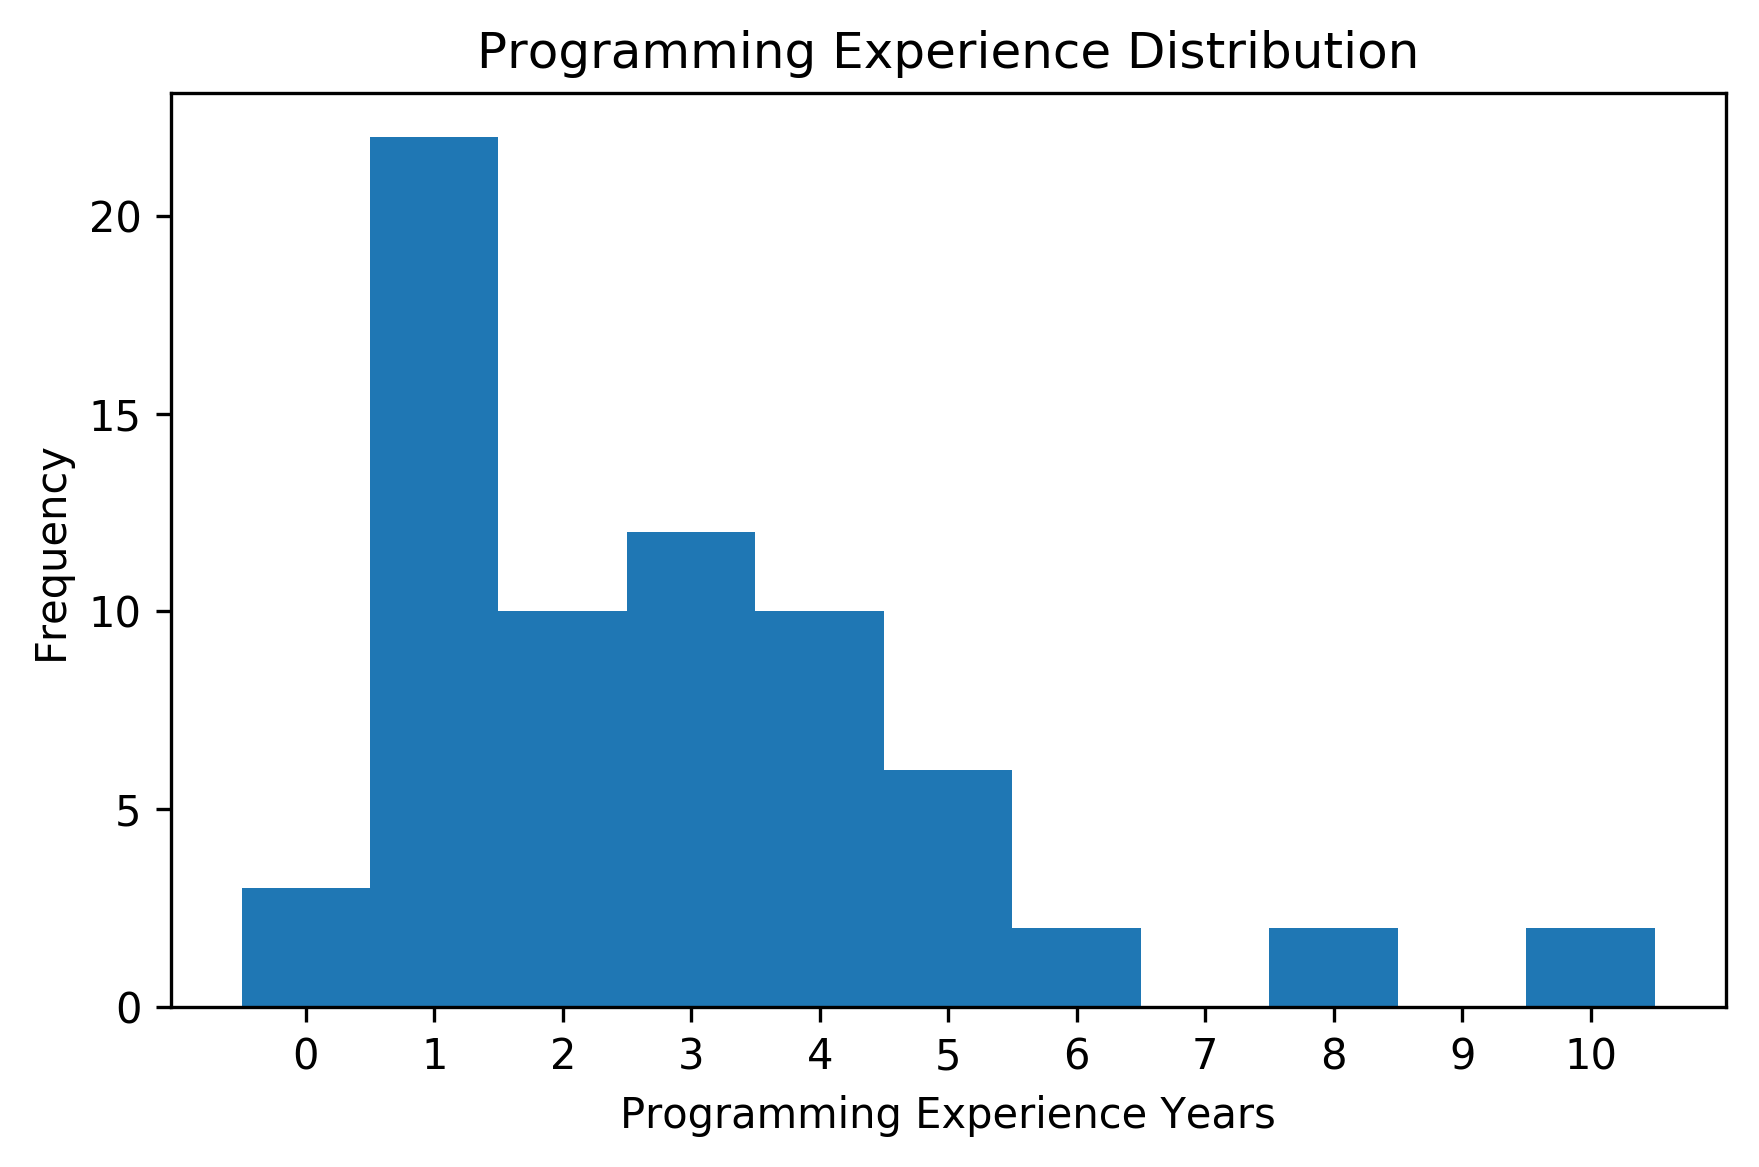
\includegraphics[width=3in]{./figs/programming-experience-distribution.png}
    \caption{Frequency histogram displaying all 69 responses for the programming experience question. A value of 10 means 10 or more years.}
    \label{PROG_EXP}
  \end{figure}
  
  \begin{figure}[ht]
    \centering
    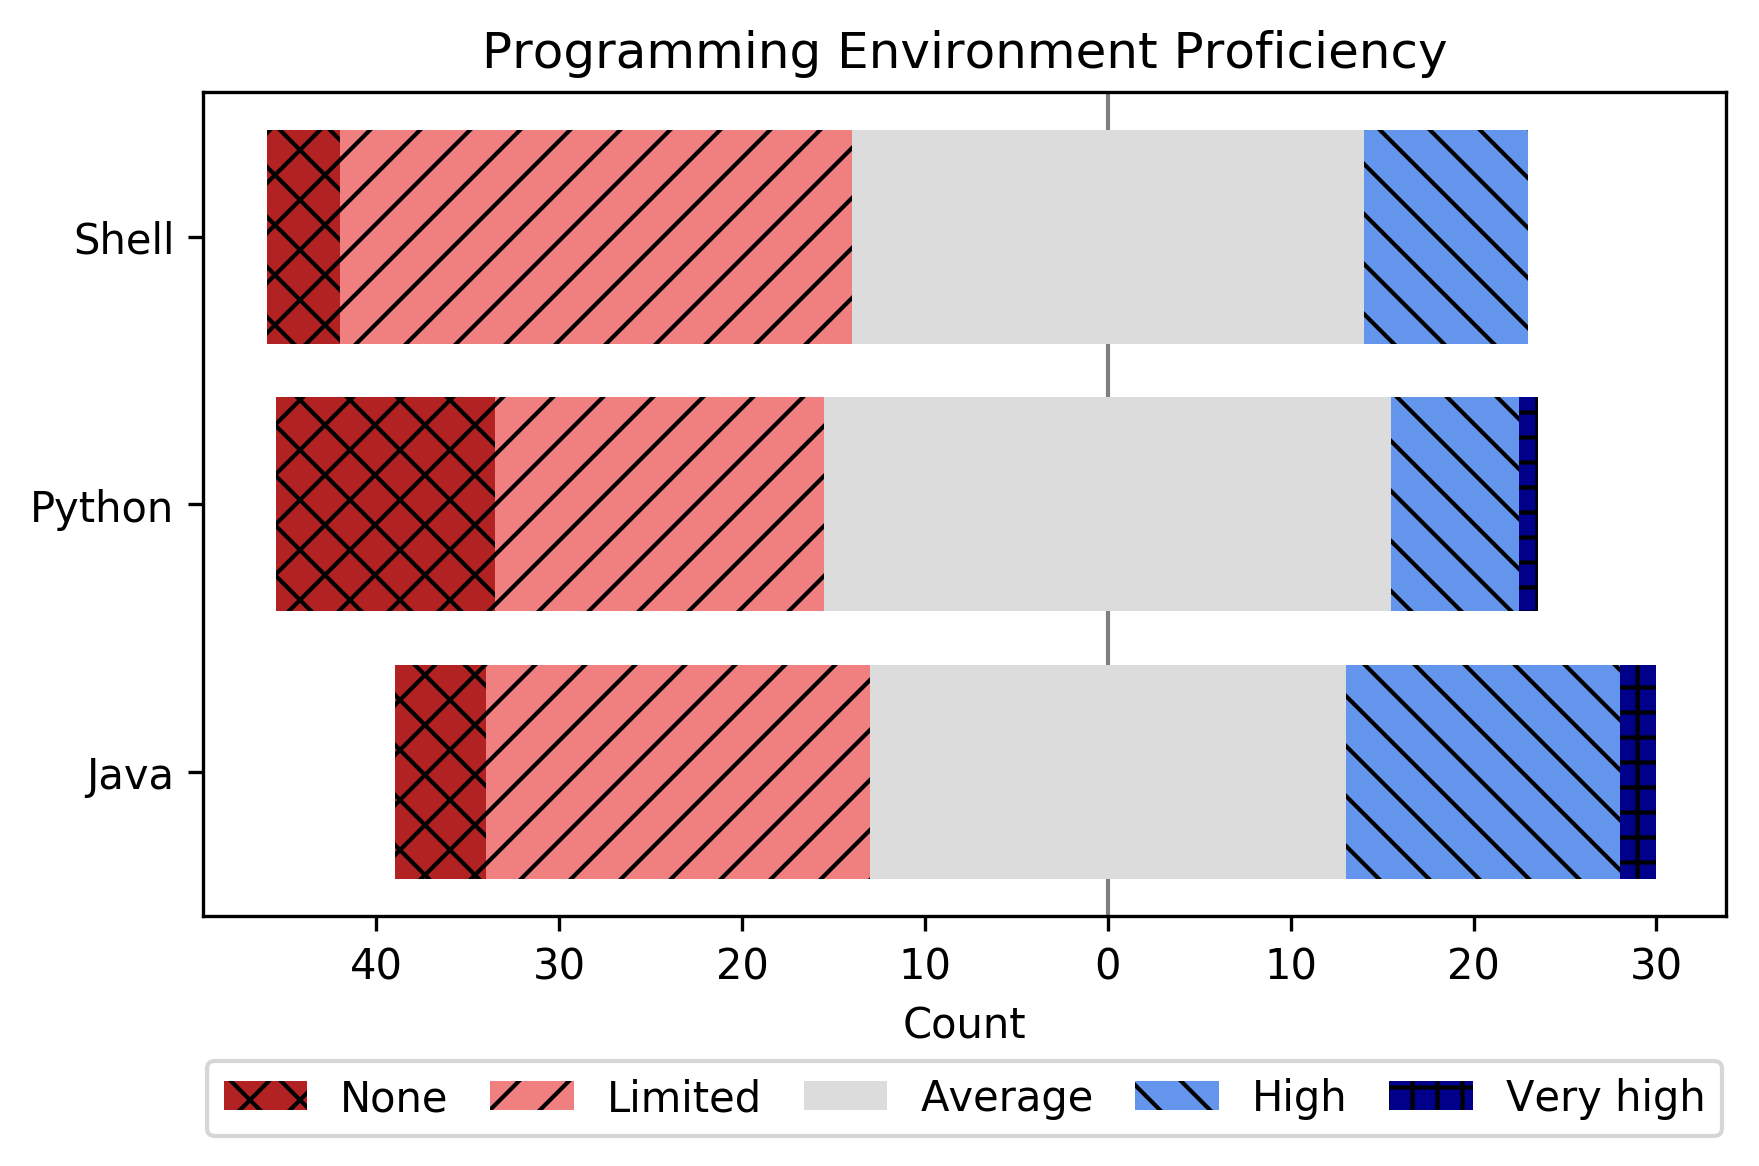
\includegraphics[width=3in]{./figs/programming-environment-proficiency.png}
    \caption{Diverging stacked bar chart \cite{HEIBERGER:DSBC:2014} displaying all 69 Likert scale responses for questions on perceived programming proficiency.}
    \label{PROG_ENV_PROF}
  \end{figure}
  
  Of the 69 participants: 55 were graduate computing students; 7 were Master of Data Science students, who do not necessarily have a computer science background; 6 were final-year undergraduate students; and 1 was a master's student of a different degree.

  Figure~\ref{PROG_EXP} shows that most (78.3\%) participants reported having 1 to 4 years of programming experience. Reflecting the diversity of the student cohort, around half of the participants reported to have limited or no proficiency in shell and Python environments, compared to around a third for Java, as seen in Figure~\ref{PROG_ENV_PROF}. There is a slightly negative correlation between Java and Python proficiency, with a Spearman's rank correlation coefficient of -0.128. The Pearson correlation coefficient was not used because the data is ordinal level, failing the test's ratio level assumption.


\subsection{Preferences and SUS Scores}
\label{PREF_SUS_SCORES}
  
  \begin{figure}[ht]
    \centering
    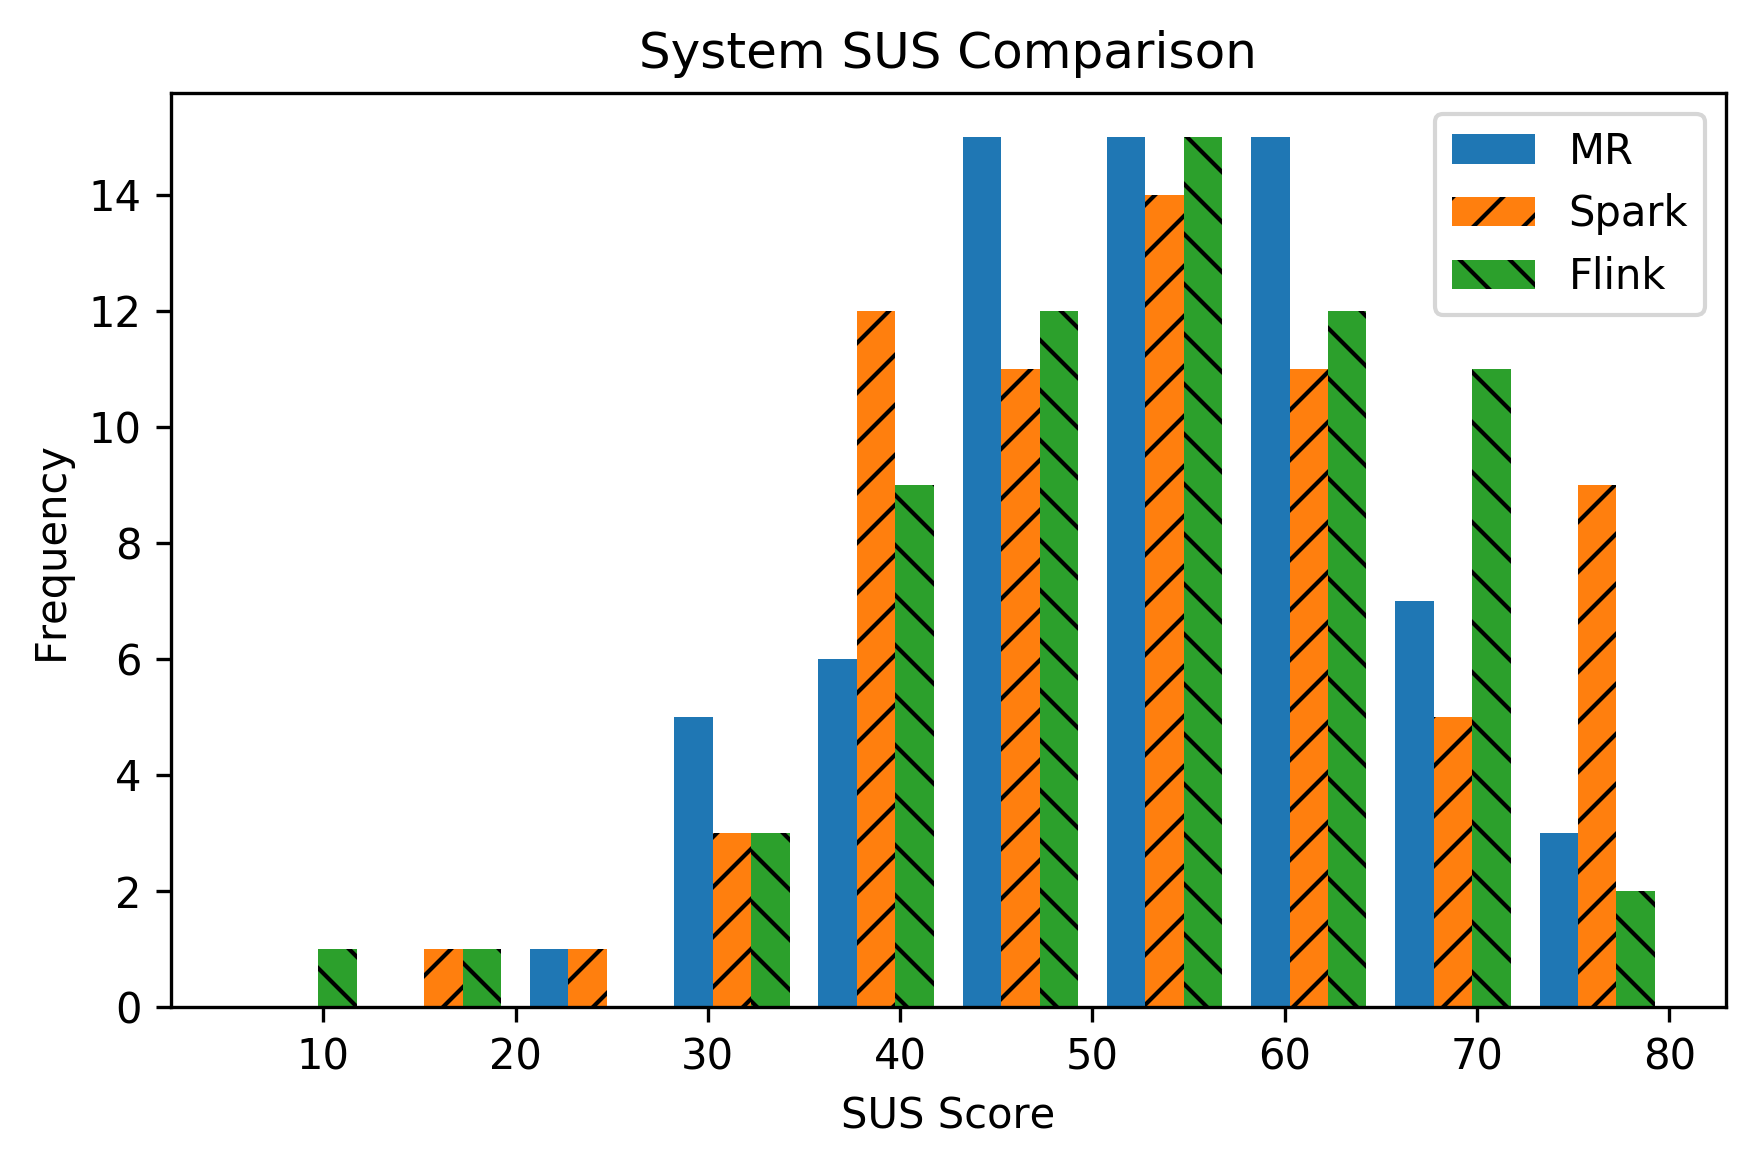
\includegraphics[width=3in]{./figs/system-sus-comparison-histogram.png}
    \caption{Frequency histogram comparing all 69 SUS scores per system (minus 7 individual incomplete responses).}
    \label{SYSTEM_SUS_HIST}
  \end{figure}
  
  \begin{figure}[ht]
    \centering
    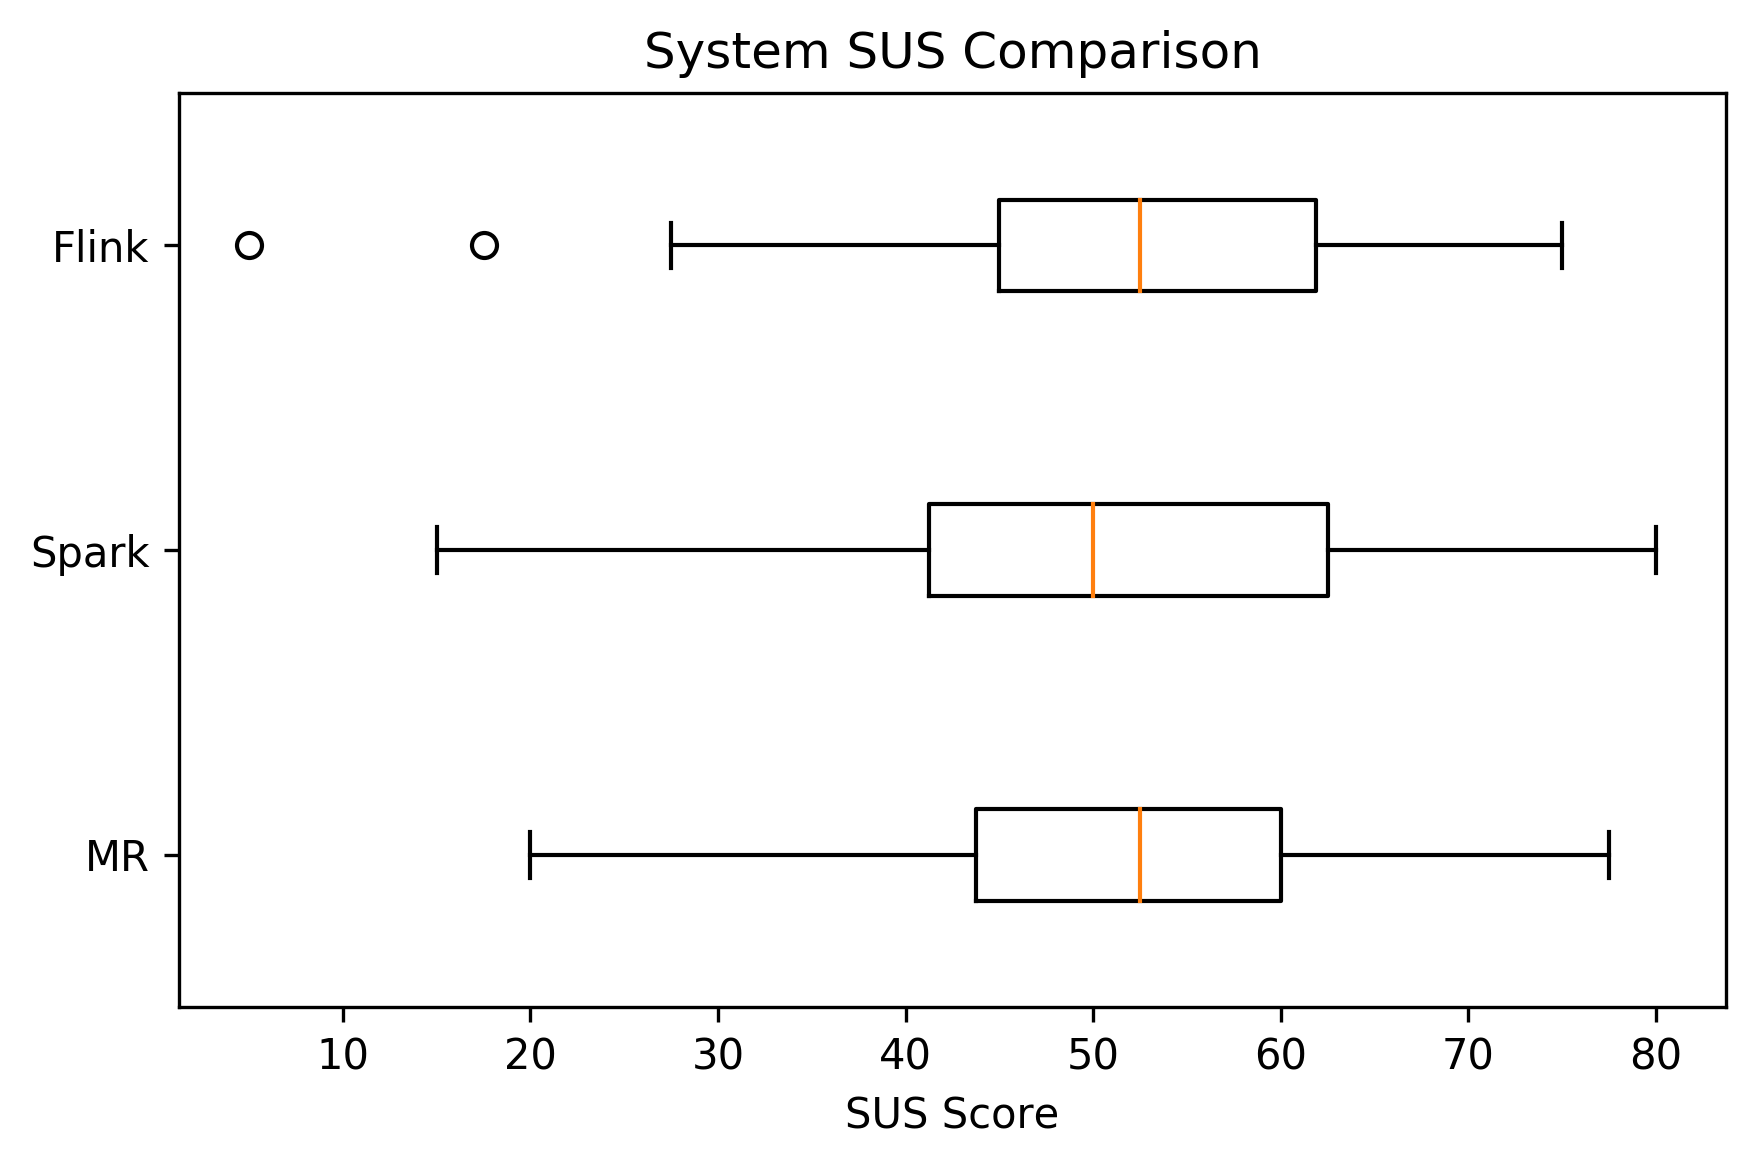
\includegraphics[width=3in]{./figs/system-sus-comparison-boxplot.png}
    \caption{Box and whisker plot comparing all 69 SUS scores per system (minus 7 individual incomplete responses). Whiskers extend to the furthest measurement within 1.5 IQR beyond quartiles. Outliers are circles.}
    \label{SYSTEM_SUS_BOX}
  \end{figure}

  Following the completion of the third survey, participants reported their system preference as: 8 (11.6\%) for Apache Hadoop MapReduce; 29 (42.0\%) for Apache Spark; and 32 (46.4\%) for Apache Flink. This is strong evidence that Spark and Flink were preferred over Hadoop MapReduce.
  
  The difference was similarly pronounced among data science students where 5 of 7 preferred Flink over Spark or MapReduce. However we note that four of those five students did use Flink in assignment~2 before using Spark, which could have an influence, as Section~\ref{ASSIGNMENT_INFLUENCE} will show. Due to the small amount of data in this context there was no applicable significance test. 
  
  The SUS scores reveal little information, with all systems sharing similar distributions and quartiles, as visible in Figures~\ref{SYSTEM_SUS_HIST} and~\ref{SYSTEM_SUS_BOX}. This can be supported by a Friedman test of all participants' three system SUS scores, resulting in a probability ($p$) value of 0.943, which suggests that there is no statistically significant difference between the systems. One-way ANOVA of repeated measures was not used because the data was nonparametric. More specifically, the hypothesis that Apache Flink scores come from a population with a normal distribution can be rejected with a Shapiro-Wilk $p$-value of 0.039 at a significance level of 0.05, and also have outliers as visible in Figure~\ref{SYSTEM_SUS_BOX}. (Hadoop MapReduce and Apache Spark have Shapiro-Wilk $p$-values of 0.767 and 0.352 respectively.)

  While participants have strongly suggested preference of Spark or Flink over MapReduce, there is no clear distinction between the two data processing systems themselves. It also means that the SUS, though a standard measure for system usability, appears to poorly correlate with perceived preferences in this context, as its lack of difference between the systems does not at all reflect the strong separation of MapReduce.


\subsection{Influence of Assignments}
\label{ASSIGNMENT_INFLUENCE}
  
  \begin{figure}[ht]
    \centering
    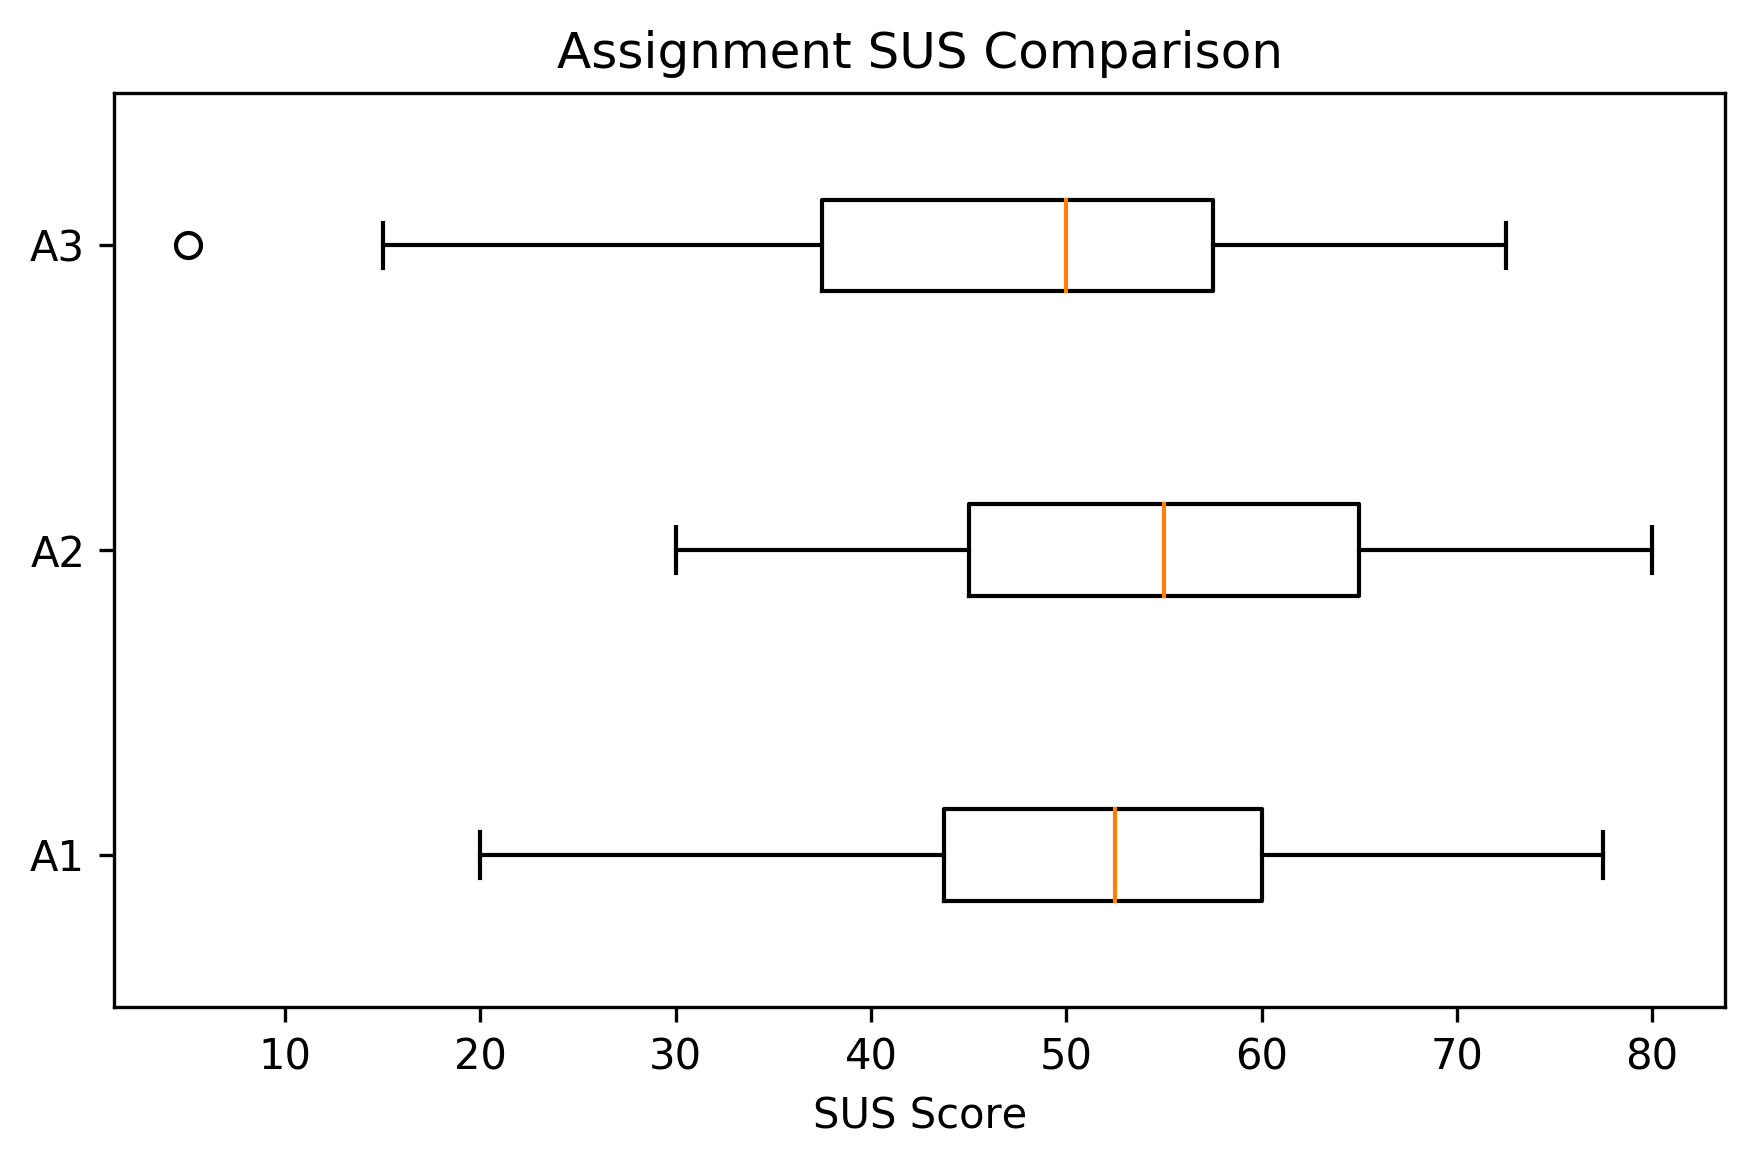
\includegraphics[width=3in]{./figs/assignment-sus-comparison.png}
    \caption{Box and whisker plot comparing all 69 SUS scores per assignment (minus 7 individual incomplete responses). Whiskers extend to the furthest measurement within 1.5 IQR beyond quartiles. Outliers are circles.}
    \label{ASSIGNMENT_SUS}
  \end{figure}
  
  \begin{figure}[ht]
    \centering
    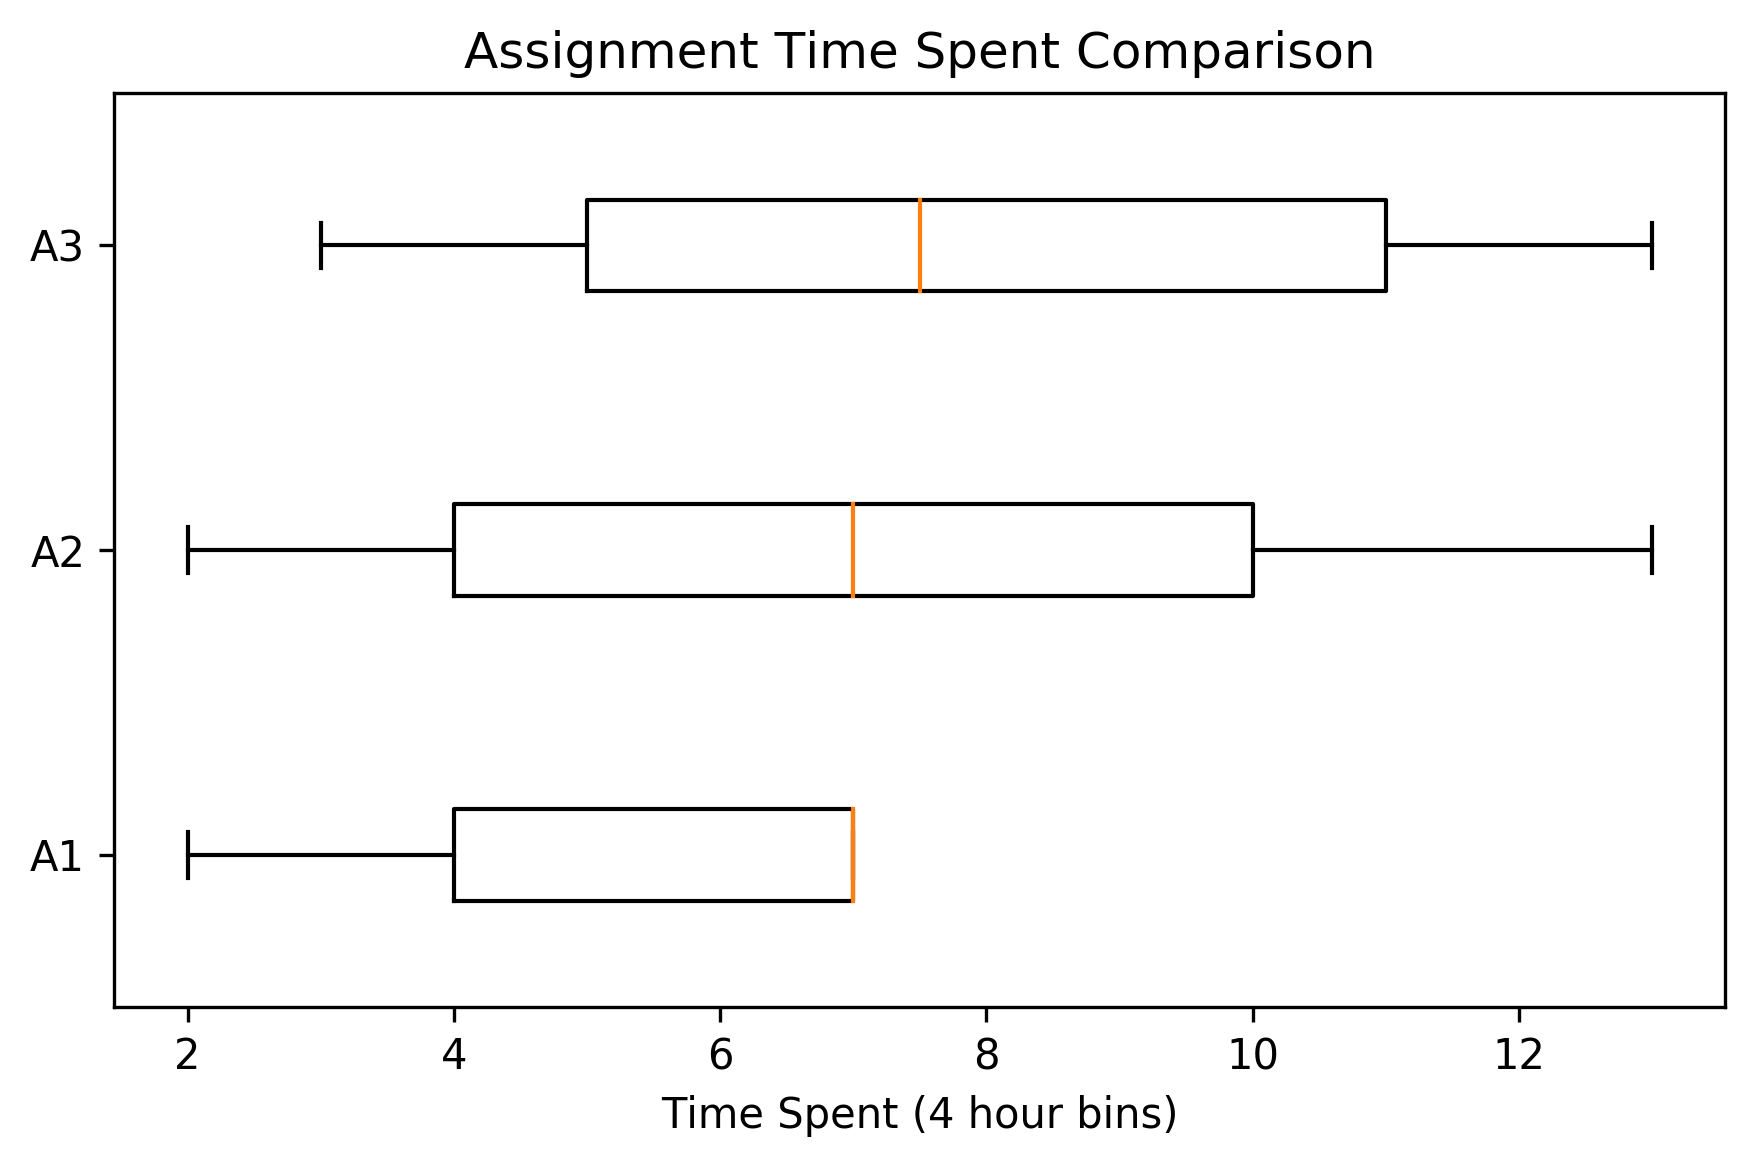
\includegraphics[width=3in]{./figs/assignment-time-comparison-boxplot.png}
    \caption{Box and whisker plot comparing all 69 amounts of time spent per assignment (minus 2 individual incomplete responses). Whiskers extend to the furthest measurement within 1.5 IQR beyond quartiles. A value of 3 means 8-12 hours, and 13 means 48+ hours. Assignment 1 was limited to value 7 or 24+ hours.}
    \label{ASSIGNMENT_TIME_BOX}
  \end{figure}
  
  \begin{figure}[ht]
    \centering
    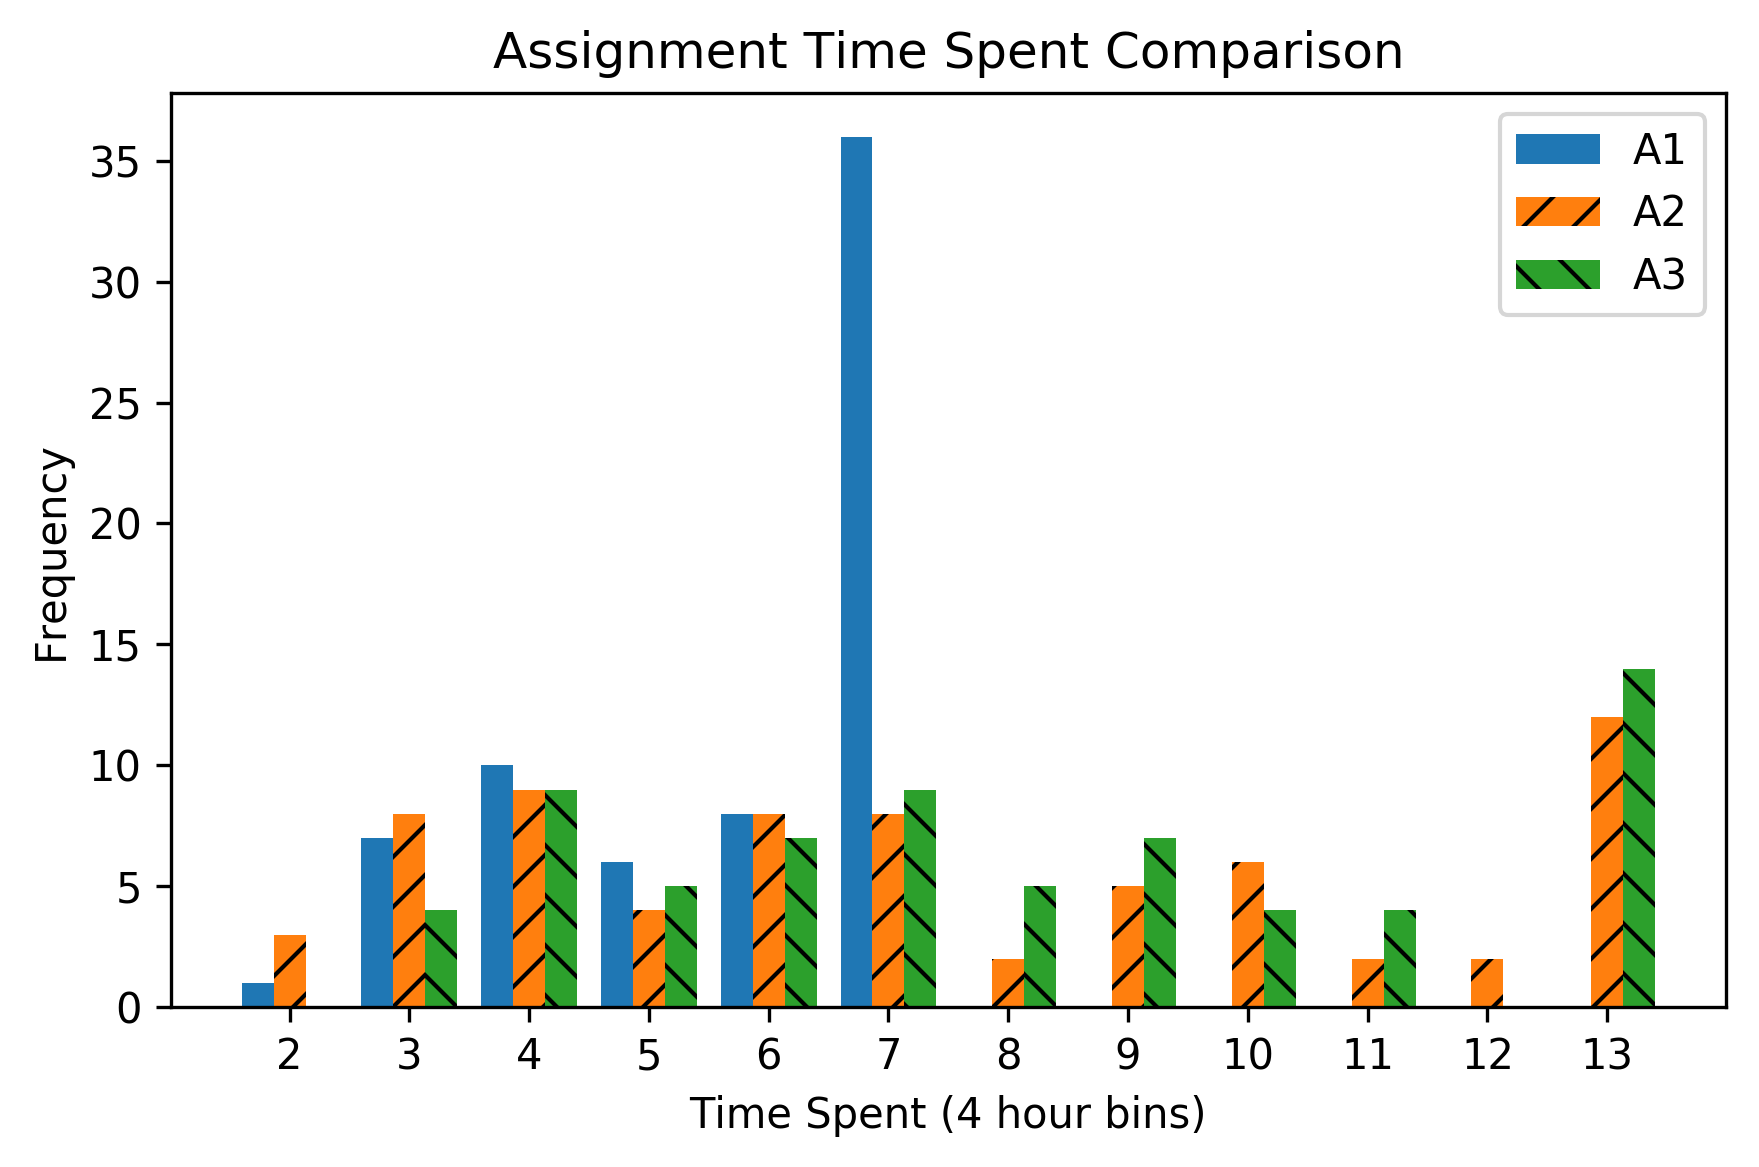
\includegraphics[width=3in]{./figs/assignment-time-comparison-histogram.png}
    \caption{Frequency histogram comparing all 69 amounts of time spent per assignment (minus 2 individual incomplete responses). A value of 3 means 8-12 hours, and 13 means 48+ hours. Assignment 1 was limited to value 7 or 24+ hours.}
    \label{ASSIGNMENT_TIME_HIST}
  \end{figure}

  The usage of a crossed A/B test in assignments~2 and~3 means the SUS scores per assignment differ from the SUS scores per system. The difference in SUS scores is more clearly pronounced per assignment than per system, as visible by comparing Figure~\ref{ASSIGNMENT_SUS} to Figure~\ref{SYSTEM_SUS_BOX}. It appears as though assignment~2 had the highest relative SUS scores, and assignment~3 the lowest. This is supported by a Friedman test of all participants' three assignment SUS scores, resulting in a $p$-value of 0.025, which suggests a statistically significant difference at a significance level of 0.05.
  
  More than half of the participants (39 participants or 56.5\%) preferred the system they used in assignment~2, compared to 22 (31.9\%) for assignment~3 (with the other 8 (11.6\%) preferring Apache Hadoop MapReduce), which is quite a noteworthy difference. However, it is difficult to reason about this difference, as there is no clear distinction as to whether the difference is due to some form of a first-system-used bias or differences in assignment difficulty (as described in Section~\ref{USABILITY_STUDY}). Figure~\ref{ASSIGNMENT_TIME_BOX} shows the time spent working on assignments, which provides a hint as to potential differences in assignment difficulty, wherein assignment~3 appeared to require slightly more time than assignment~2. However, this claim is not supported by a one-sided sign test with plus representing participants who spent more time on assignment~3 than~2, and minus otherwise, resulting in a $p$-value of 0.358. The sign test is used because the data is non-normal and asymmetrical, as clearly visible in Figure~\ref{ASSIGNMENT_TIME_HIST}, ruling out the paired t-test due to it being a parametric test, and the Wilcoxon signed-rank test due to it having high Type I error rates when used with asymmetric data.
  
  While we suspect assignment difficulty and `first-used advantages' could have affected perceived preferences, we have not been able to quantitatively explain the significant difference between assignment SUS scores, nor any link between SUS scores and assignment preferences. With that being said, the crossed A/B test that was used should have helped to reduce any effect of these biases on the systems themselves.


\subsection{Programming Duration versus System}
\label{INF_PROG_DURATION_VS_SYSTEM}
  
  \begin{figure}[ht]
    \centering
    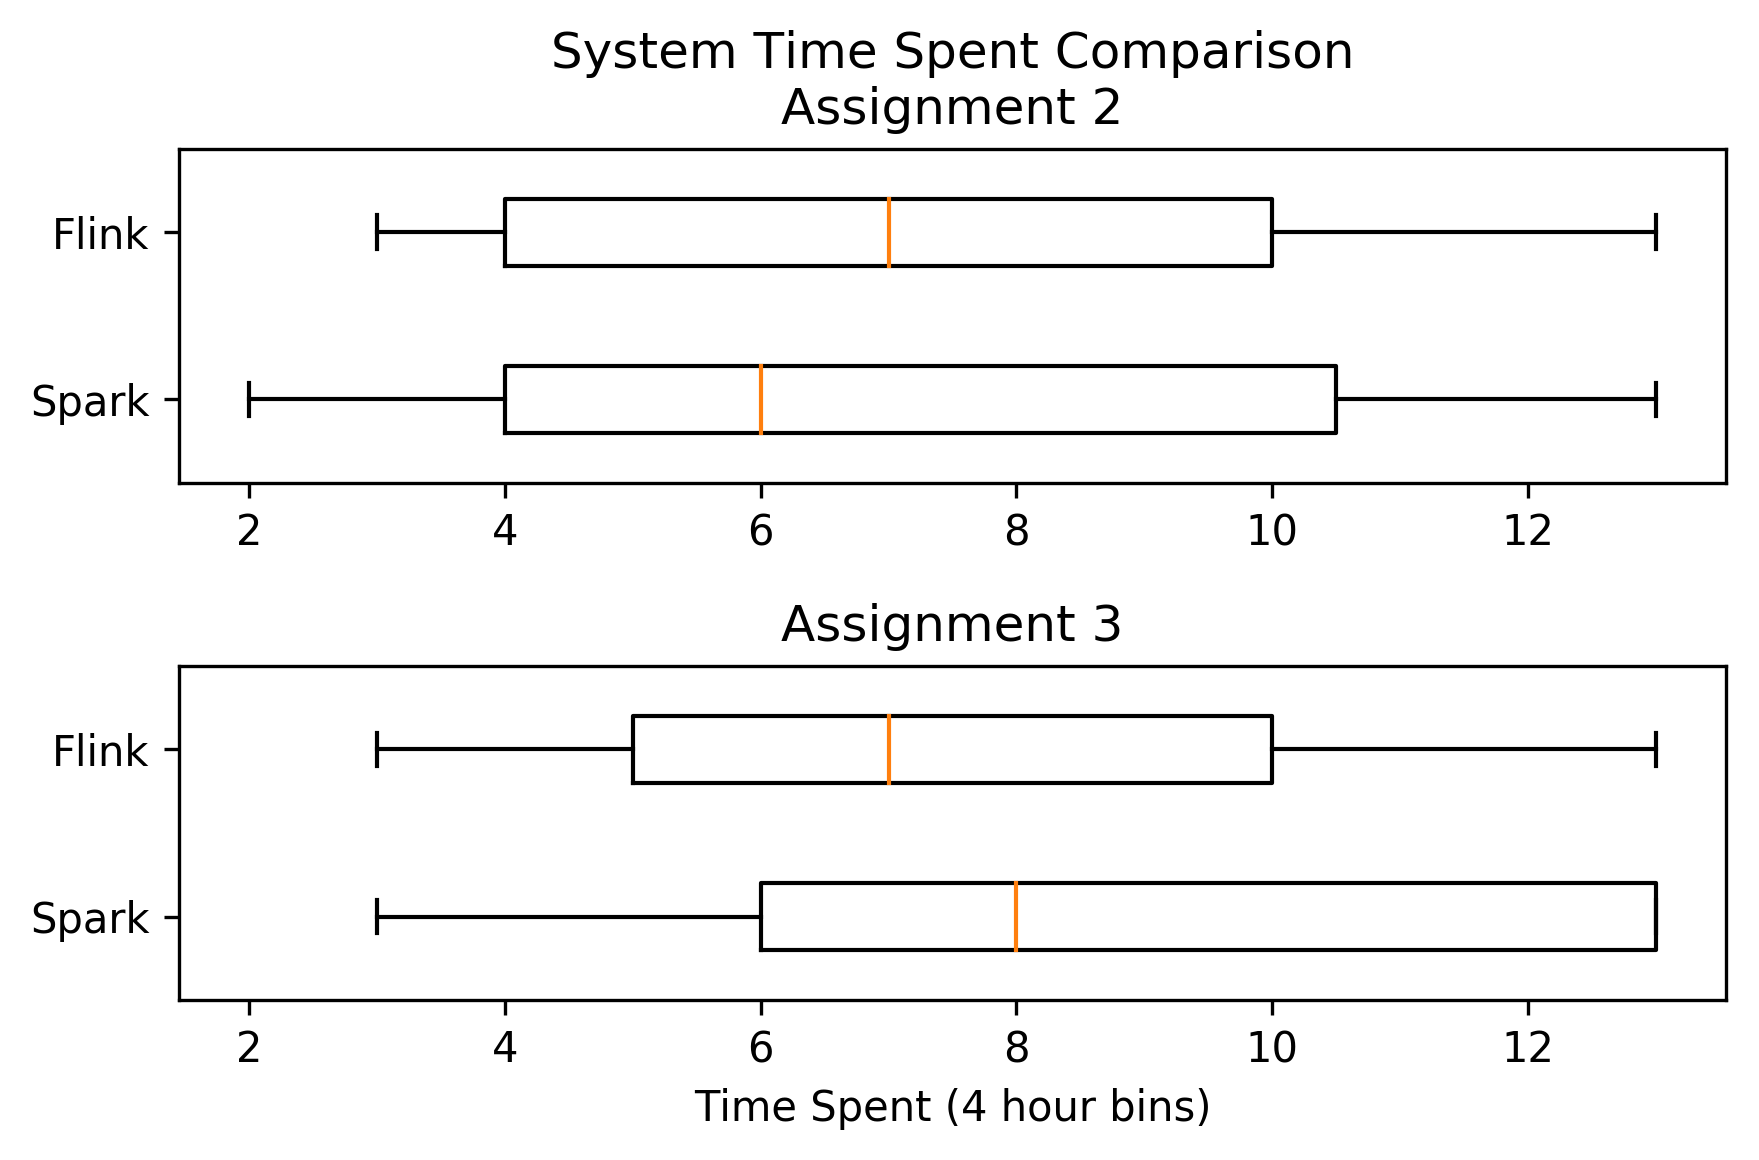
\includegraphics[width=3in]{./figs/assignment-system-time-comparison-boxplot.png}
    \caption{Box and whisker plots for assignments 2 and 3 comparing all 69 amounts of time spent per assignment (minus 1 individual incomplete response). Whiskers extend to the furthest measurement within 1.5 IQR beyond quartiles. A value of 3 means 8-12 hours, and 13 means 48+ hours.}
    \label{ASSIGNMENT_SYSTEM_TIME_BOX}
  \end{figure}
  
  \begin{figure}[ht]
    \centering
    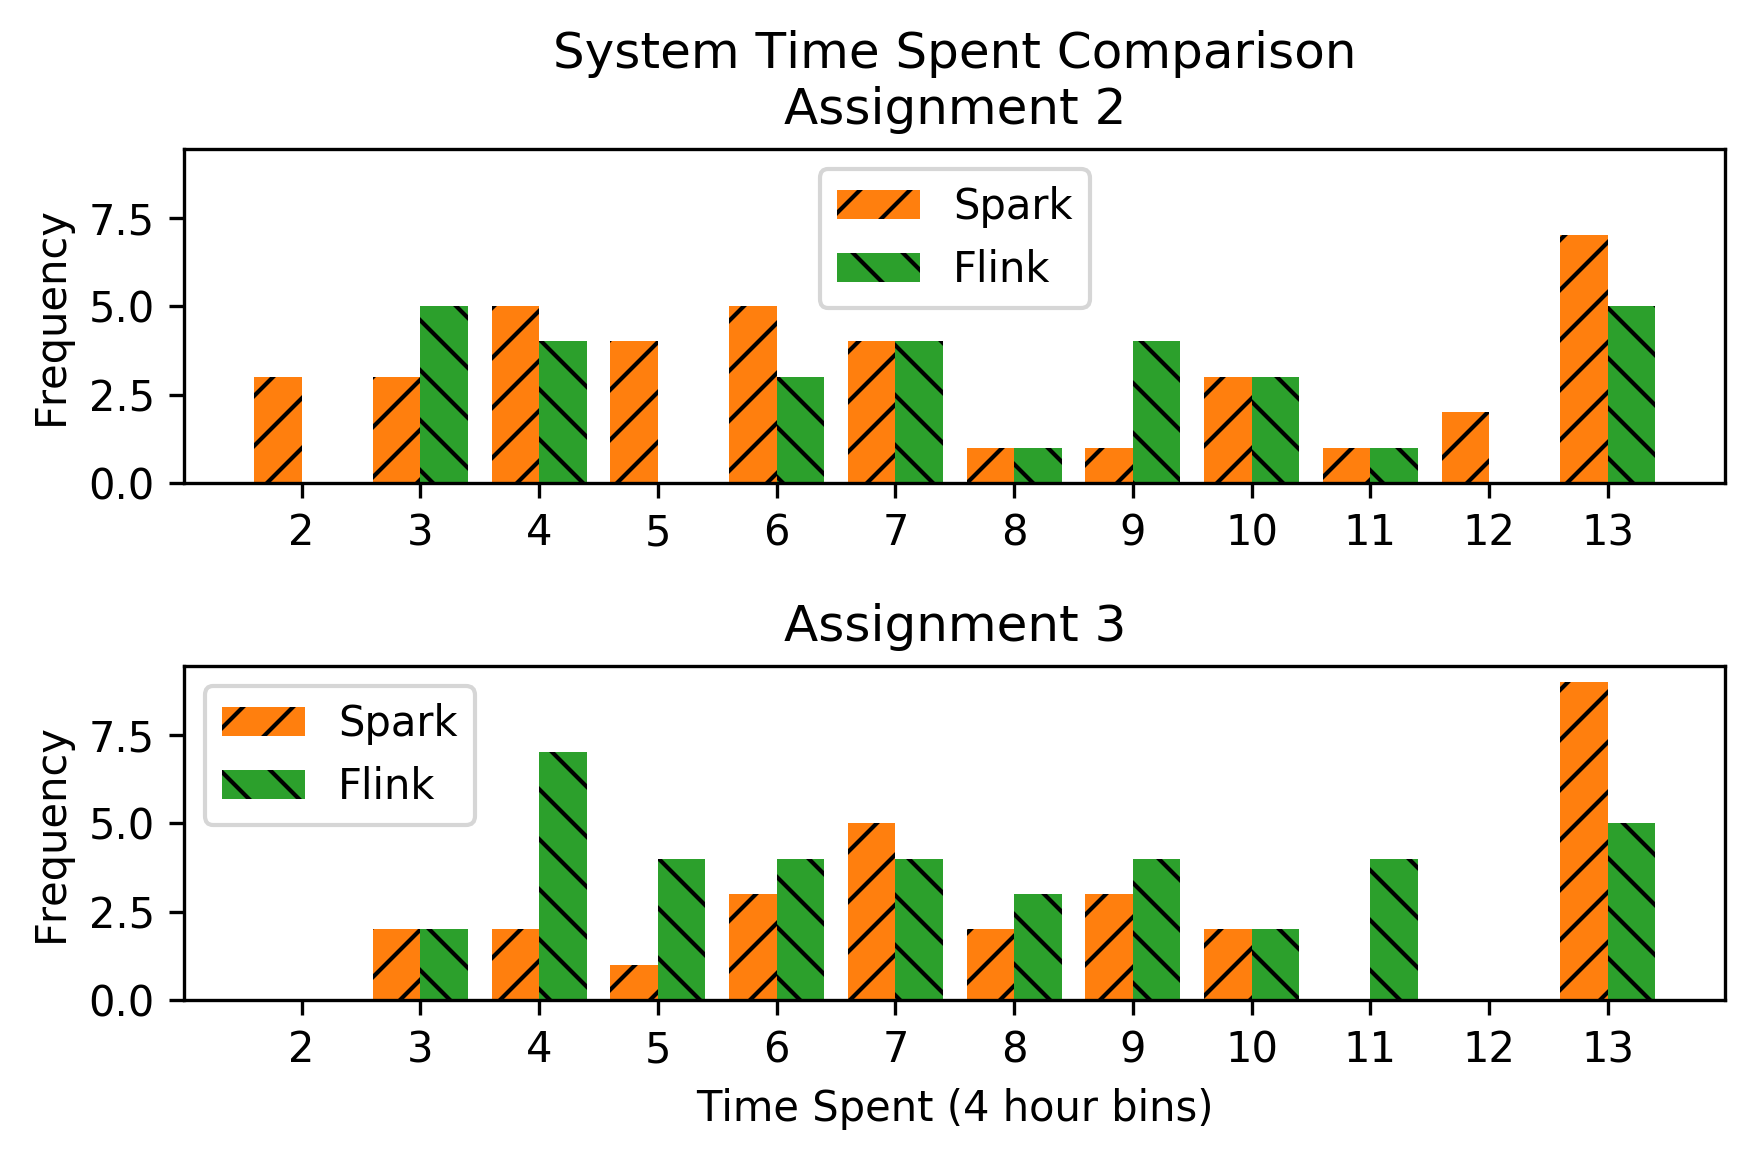
\includegraphics[width=3in]{./figs/assignment-system-time-comparison-histogram.png}
    \caption{Frequency histograms for assignments 2 and 3 comparing all 69 amounts of time spent per system (minus 1 individual incomplete response). A value of 3 means 8-12 hours, and 13 means 48+ hours.}
    \label{ASSIGNMENT_SYSTEM_TIME_HIST}
  \end{figure}
  
  Apache Hadoop MapReduce is not being included in this comparative analysis, as the data we collected for it was unfortunately inappropriate -- described in Subsection~\ref{EXEC_SURVEYS}.

  Apache Spark and Apache Flink shared similar reported development times for assignment~2, but with Flink perhaps showing slightly better results for assignment~3, which you can see in Figure~\ref{ASSIGNMENT_SYSTEM_TIME_BOX}. However, this is not supported by Mood's median tests of the two systems' (independent) time spent data, resulting in $p$-values of 0.661 for assignment~2 and 0.624 for assignment~3, and thus suggesting no statistically significant difference in either. Mood's median test is used because the data is non-normal and differs in distribution, as clearly visible in Figure~\ref{ASSIGNMENT_SYSTEM_TIME_HIST}, ruling out the one-way ANOVA due to it being a parametric test, and the Mann-Whitney U test due to it not testing changes in medians or means (but instead testing changes in distribution) when used with data of differing distributions.

  Spark and Flink do not present a significant difference in the amount of time that was required to complete either of the assignments. This shows that both systems are similarly suitable for completion of data analysis tasks like those in assignments~2 and~3.


\subsection{Influence of Programming Experience}
\label{INF_PROG_EXP}
  
  \begin{figure}[ht]
    \centering
    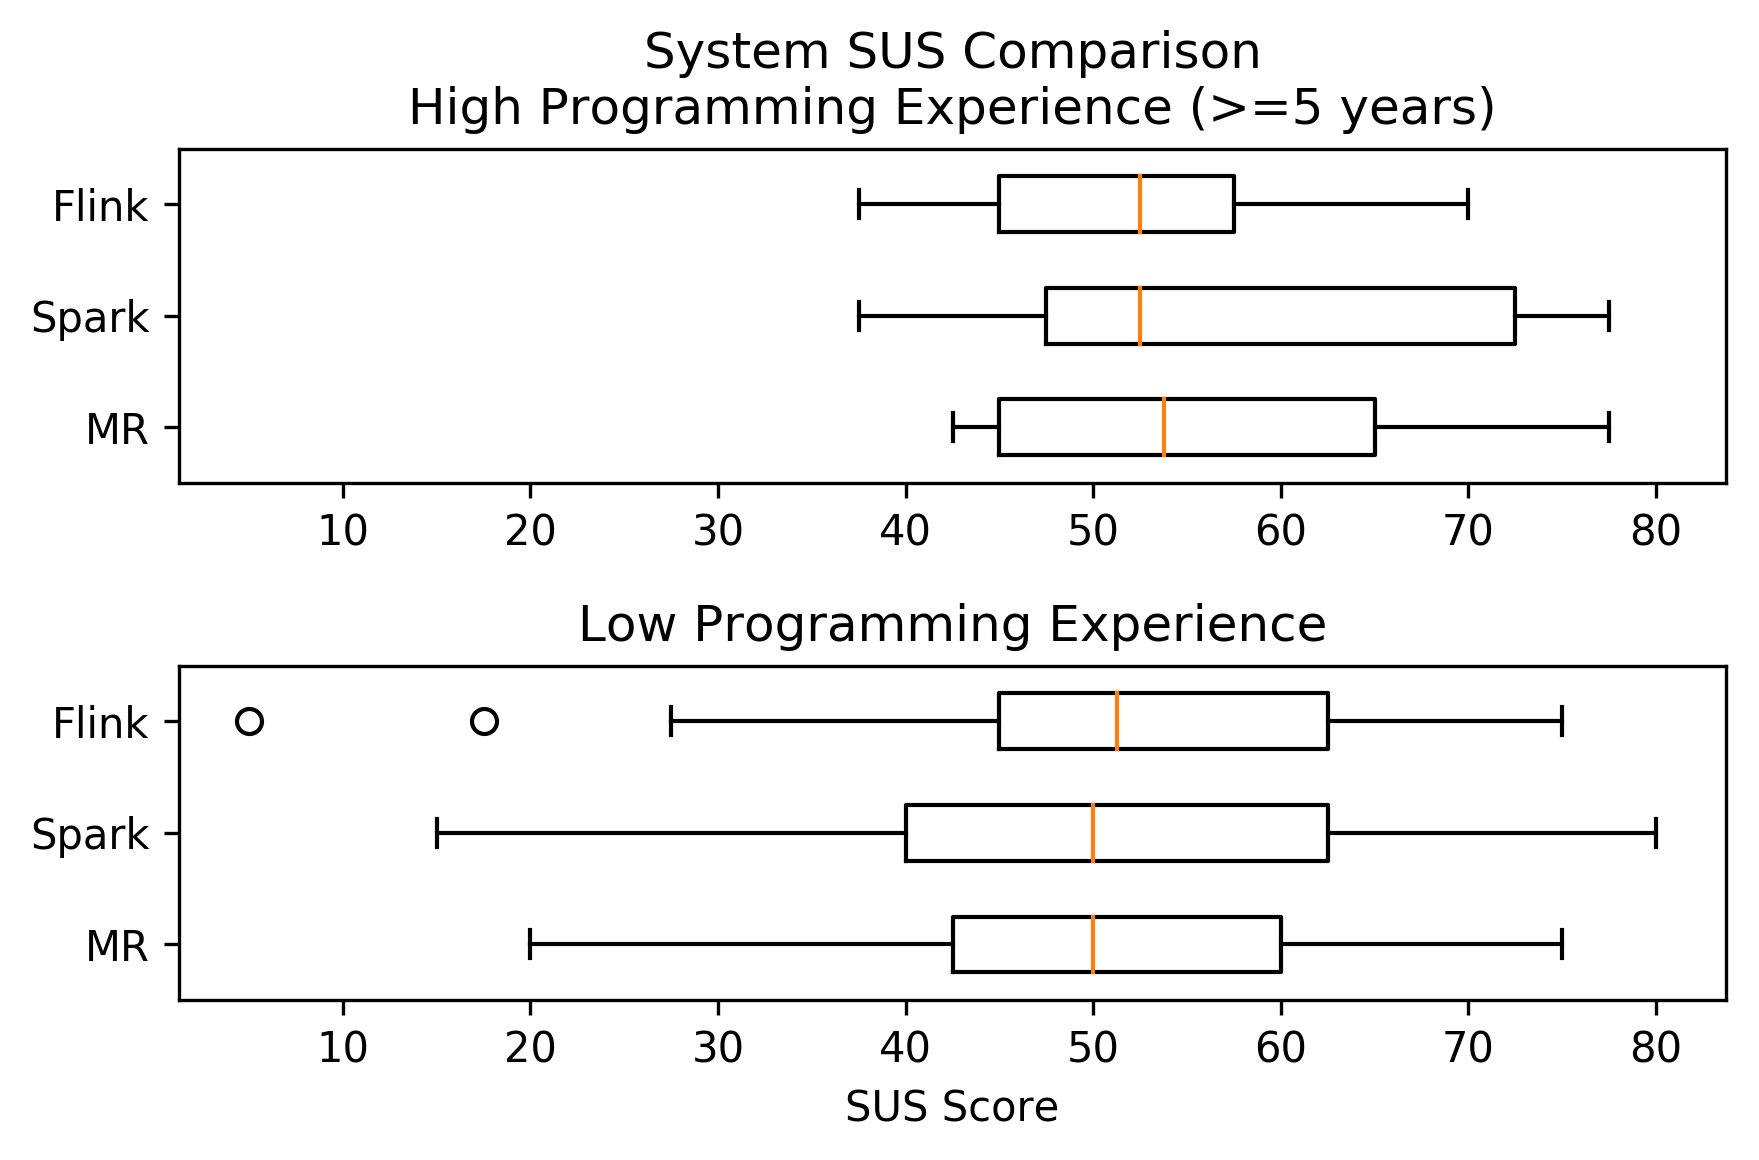
\includegraphics[width=3in]{./figs/exp-system-sus-comparison.png}
    \caption{Box and whisker plots for high (\textgreater=5 years) and low programming experience participants comparing all 69 SUS scores per system (minus 7 individual incomplete responses). Whiskers extend to the furthest measurement within 1.5 IQR beyond quartiles. Outliers are circles.}
    \label{EXP_SYSTEM_SUS}
  \end{figure}
  
  \begin{figure}[ht]
    \centering
    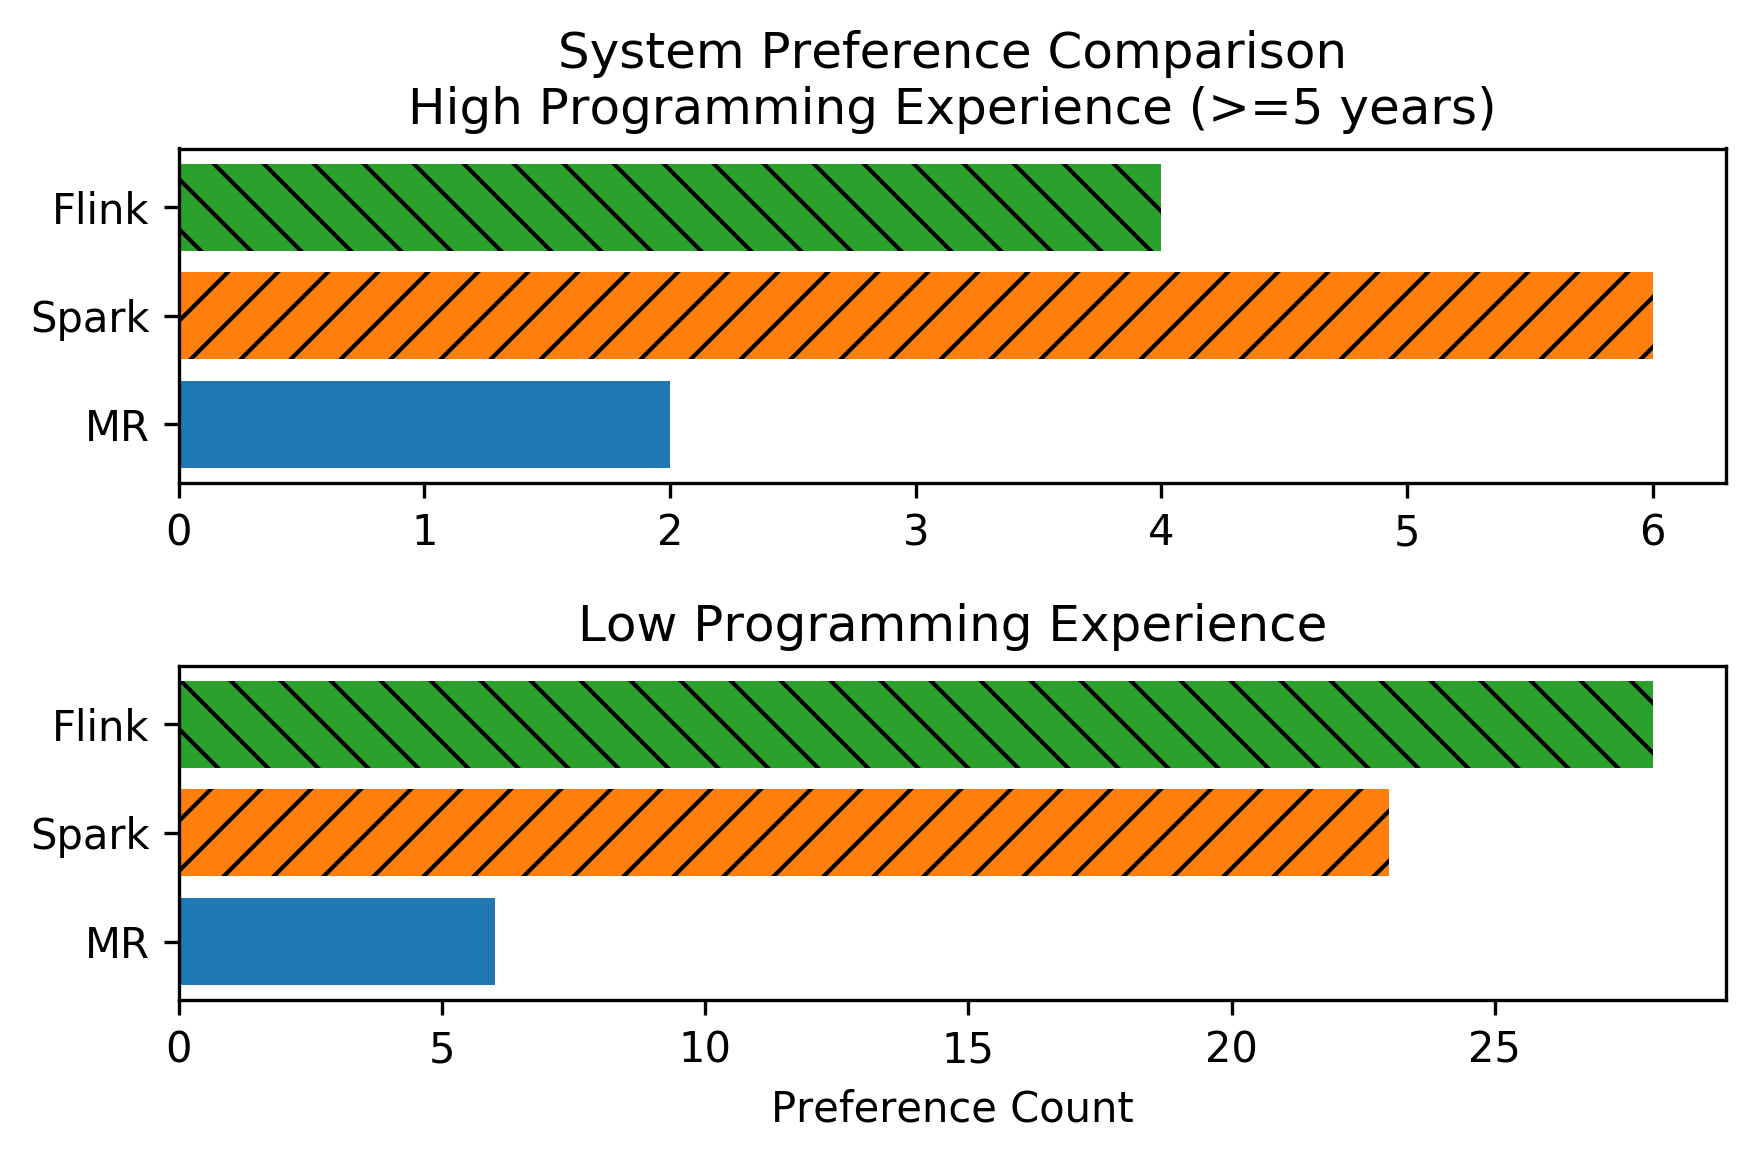
\includegraphics[width=3in]{./figs/exp-system-preference-comparison.png}
    \caption{Bar charts for high (\textgreater=5 years) and low programming experience participants comparing reported system preference counts upon completion of assignment~3. There are 69 preferences measured in total. Charts have differing Preference Count scales.}
    \label{EXP_SYSTEM_PREF}
  \end{figure}

  As previously mentioned, Figure~\ref{PROG_EXP} shows that most (78.3\%) participants reported having 1 to 4 years of programming experience. In this subsection we will consider the 12 (17.4\%) participants who reported having more than 4 years experience as being of relatively `high experience'. Their experience is distributed as so: 6 with 5 years experience, and 2 with each of 6, 8 and 10+ years experience. Is there any difference in the reported preferences or SUS scores for high experience participants compared to the majority?
  
  A comparison between the two groups' system SUS scores is shown in Figure~\ref{EXP_SYSTEM_SUS}, which does not tell much of any preference or skew. The ranges of all three systems are more dense and perhaps slightly higher overall in the high experience group, and also particularly lacking the long tail towards lower scores. However, it is difficult to indicate that it is not due to coincidence. These observations still apply, perhaps with a slight reduction in density, when moving the threshold from 5 years to 3 years and thus placing 34 (49.3\%) participants in the high experience tier.
  
  A comparison between the two groups' reported preferences is shown in Figure~\ref{EXP_SYSTEM_PREF}, which also does not tell much of any preference or skew. Hadoop MapReduce remains behind the dataflow engines, but it is difficult to reason much further. For instance, the difference in Apache Flink and Apache Spark looks quite pronounced, with Flink appearing to be less preferred to Spark in comparison to the low experience group. However, in actual fact it is only a difference of two individual preferences, which is difficult to claim as being anything other than coincidence. When moving the threshold from 5 years to 3 years and thus placing 34 (49.3\%) participants in the high experience tier, the two charts end up look nearly identical, also with very similar Preference Count scales.
  
  It was good to have collected the programming experience data as part of the survey, especially with full participation in that regard, having provided information regarding the background of participants and the diversity present in the study. However, this information did not turn out to be indicative of any pattern in reported preferences or system SUS scores.


\subsection{Influence of Programming Language}
\label{LANGUAGE_INFLUENCE}

  In the analysis thus far, participants' usage of Python or Java for each system or assignment has not been taken into account. However, it is mentioned in Section~\ref{EXECUTION} that learning materials, or more specifically tutorial exercises and sample assignment solutions, were not successfully created for Apache Flink; that students were recommended not to use Python for Flink; and that this recommendation was followed by all students. Unfortunately, this presents an inconsistency in the experiment which could bias some of the findings. This subsection will explore said biases by comparing the previous analyses with a repetition of them that excluded all Python user data.
  
  Of the 69 participants whose data was used in the above analyses, 32 (46.4\%) had used Python for either or both of assignment~1 (Hadoop MapReduce) or the assignment in which they used Apache Spark. Excluding this data leaves 37 records to work with. Furthermore, the crossed A/B test that was employed did not take programming language usage into account, and thus the Python records removed could have further produced skew in that regard. With 69 records the Spark vs. Flink usage split for assignment~2 (and conversely for assignment~3) is 39 vs. 30 (56.5\% vs. 43.5\%) respectively, skewed due to students' requests to switch to Apache Spark as described in Section~\ref{EXECUTION}, whereas with 37 records it is 23 vs. 14 (62.2\% vs. 37.8\%) respectively. Flink is 9 users behind Spark (for assignment~2) in both cases, however this difference is more pronounced as a percentage in the latter case.
  
  Of the subsections that were analysed earlier, noteworthy differences were only apparent in relation to the background of participants, and their reported system preferences.
  
\subsubsection{Background of Participants}
  
  \begin{figure}[ht]
    \centering
    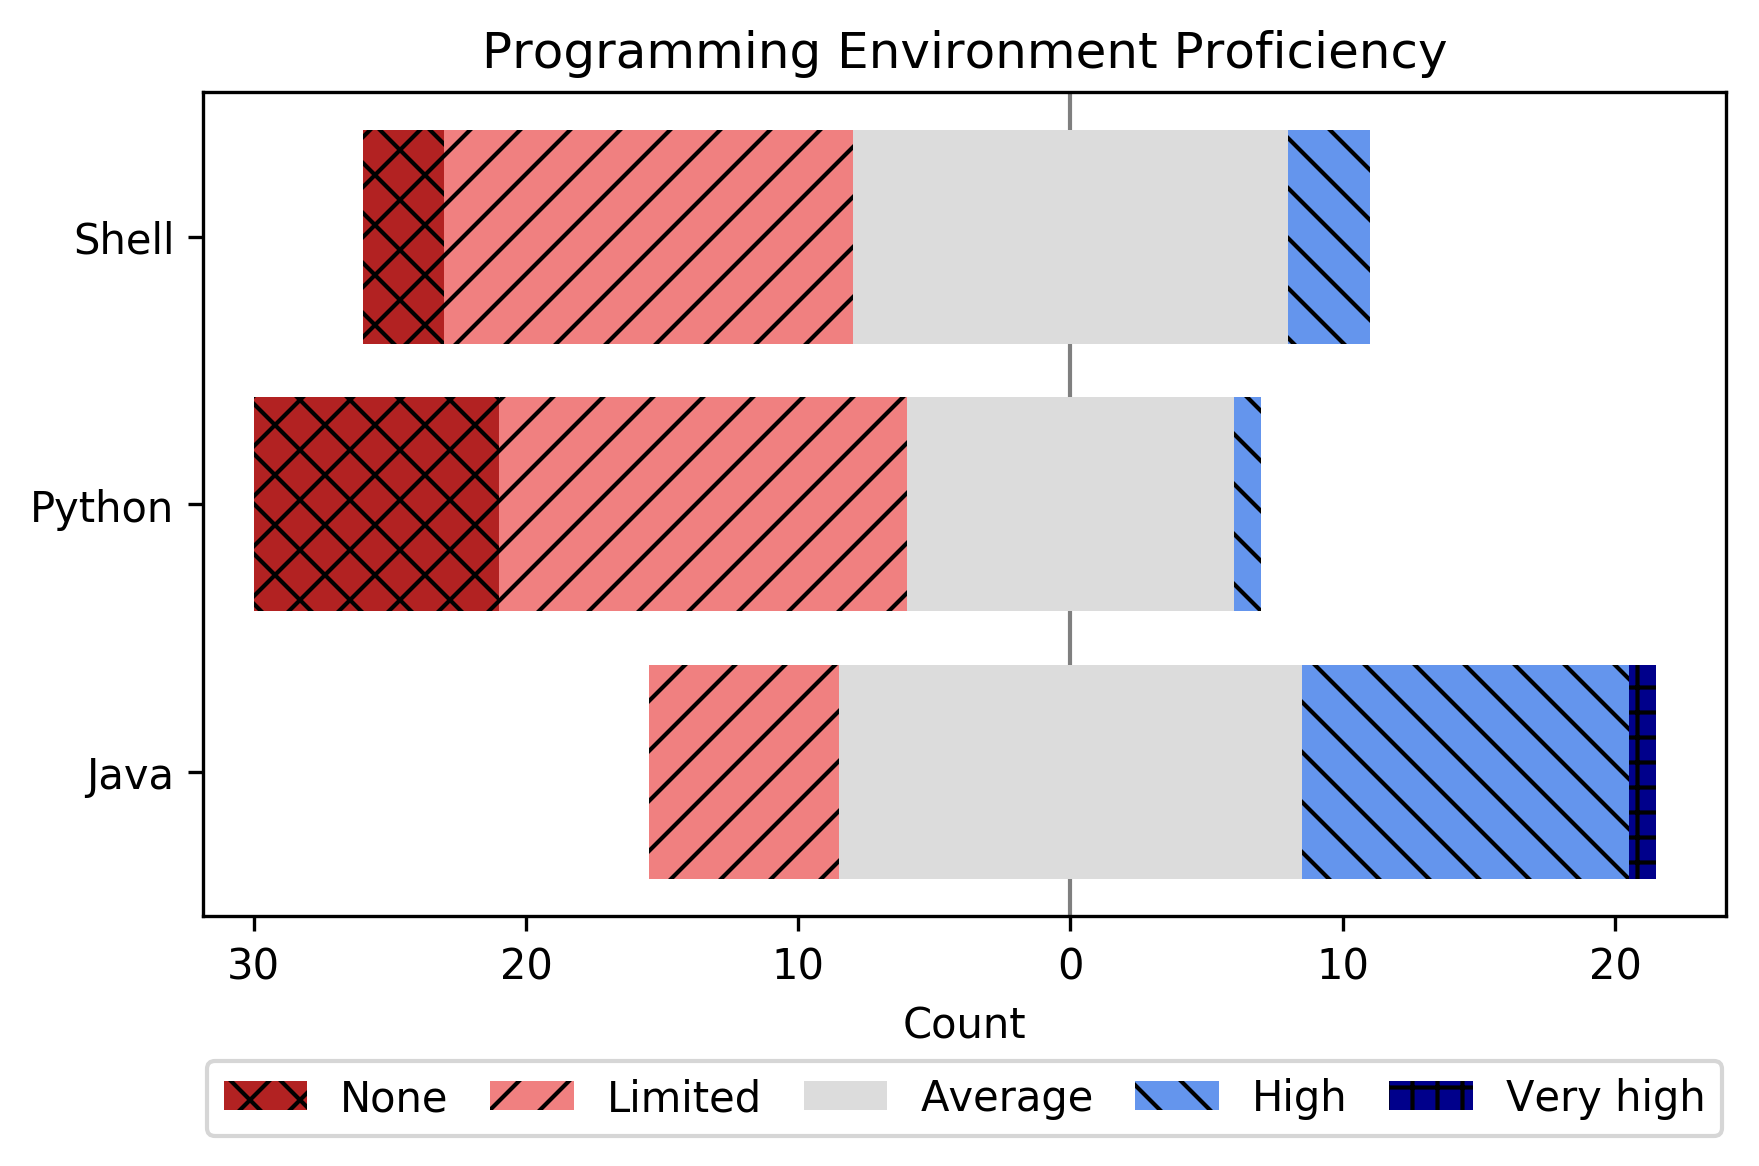
\includegraphics[width=3in]{./figs/nopy-programming-environment-proficiency.png}
    \caption{Diverging stacked bar chart \cite{HEIBERGER:DSBC:2014} displaying all 37 (Python user data excluded) Likert scale responses for questions on perceived programming proficiency.}
    \label{NOPY_PROG_ENV_PROF}
  \end{figure}

  Of the 37 participants: 33 were graduate computing students; 1 (compared to 7) was a Master of Data Science student; 2 were final-year undergraduate students; and 1 was a master's student of a different degree. Furthermore, Figure~\ref{NOPY_PROG_ENV_PROF} (compared to Figure~\ref{PROG_ENV_PROF}) shows the dominance of Java among the cohort, also with substantially more participants reporting having limited or no Python proficiency than average or higher.
  
  This apparent reduction in diversity may be due to individuals in this cohort having been more likely to have come from a computer science background, where compiled and object-oriented programming languages would be of a larger focus than scripting languages -- which is what we observe Python to be commonly taught as, despite it also being object-oriented. Unfortunately, this representation may not effectively capture the experiences of interdisciplinary users, as has been one of our intentions in conducting this study.


\subsubsection{Preferences}

  Following completion of the third survey, participants reported their system preference as: 4 (10.8\%) for Hadoop MapReduce; 12 (32.4\%) for Apache Spark; and 21 (56.8\%) for Apache Flink. While this result is similar to the full (Python included) data set in how MapReduce is behind in comparison to the dataflow engines, it differs from having Spark and Flink on a very close footing to instead placing Flink quite noticeably ahead as the participants' preferred system.
  
  This difference seems to make sense considering that Python users likely felt inconvenienced by the inability to use Python for Flink in comparison to Spark or MapReduce, thus reducing Flink's popularity among the full cohort. With Python users excluded from analysis, it has now become apparent that Flink is preferred over Spark among Java users.
  
  Unfortunately, as described in Section~\ref{EXEC_SURVEYS}, there is little information available from participants to justify these reported preferences, and so we can make no conclusion as to why Java users may have preferred Flink over Spark, especially considering the similarities in their usage as described in Section~\ref{SYSTEMS}. The key difference in usage that we could think of was in Flink's availability of \texttt{IterativeDataSet}, which could have been used in solving both assignments~2 and~3.
  
  With the full data set it was apparent that participants tended to prefer the system they used for assignment~2 more than assignment~3, as described in Section~\ref{ASSIGNMENT_INFLUENCE}. With Python data excluded, this changes to having 17 (45.9\%) participants preferring the system used for assignment~2 compared to 16 (43.2\%) for assignment~3 (with the other 4 (10.8\%) preferring MapReduce). It makes sense that assignment~3 gained preference considering the skewed crossed A/B test distribution, where more participants used Flink for assignment~3, in combination with participants' higher preference of Flink. This means that although reported preferences put assignments~2 and~3 on similar proportions, it remains likely that assignment~3 was somehow disadvantaged.


\subsection{Individual SUS Statements}
\label{SUS_INDIV}
  
  \begin{figure}[ht]
    \centering
    \makebox[\textwidth][c]{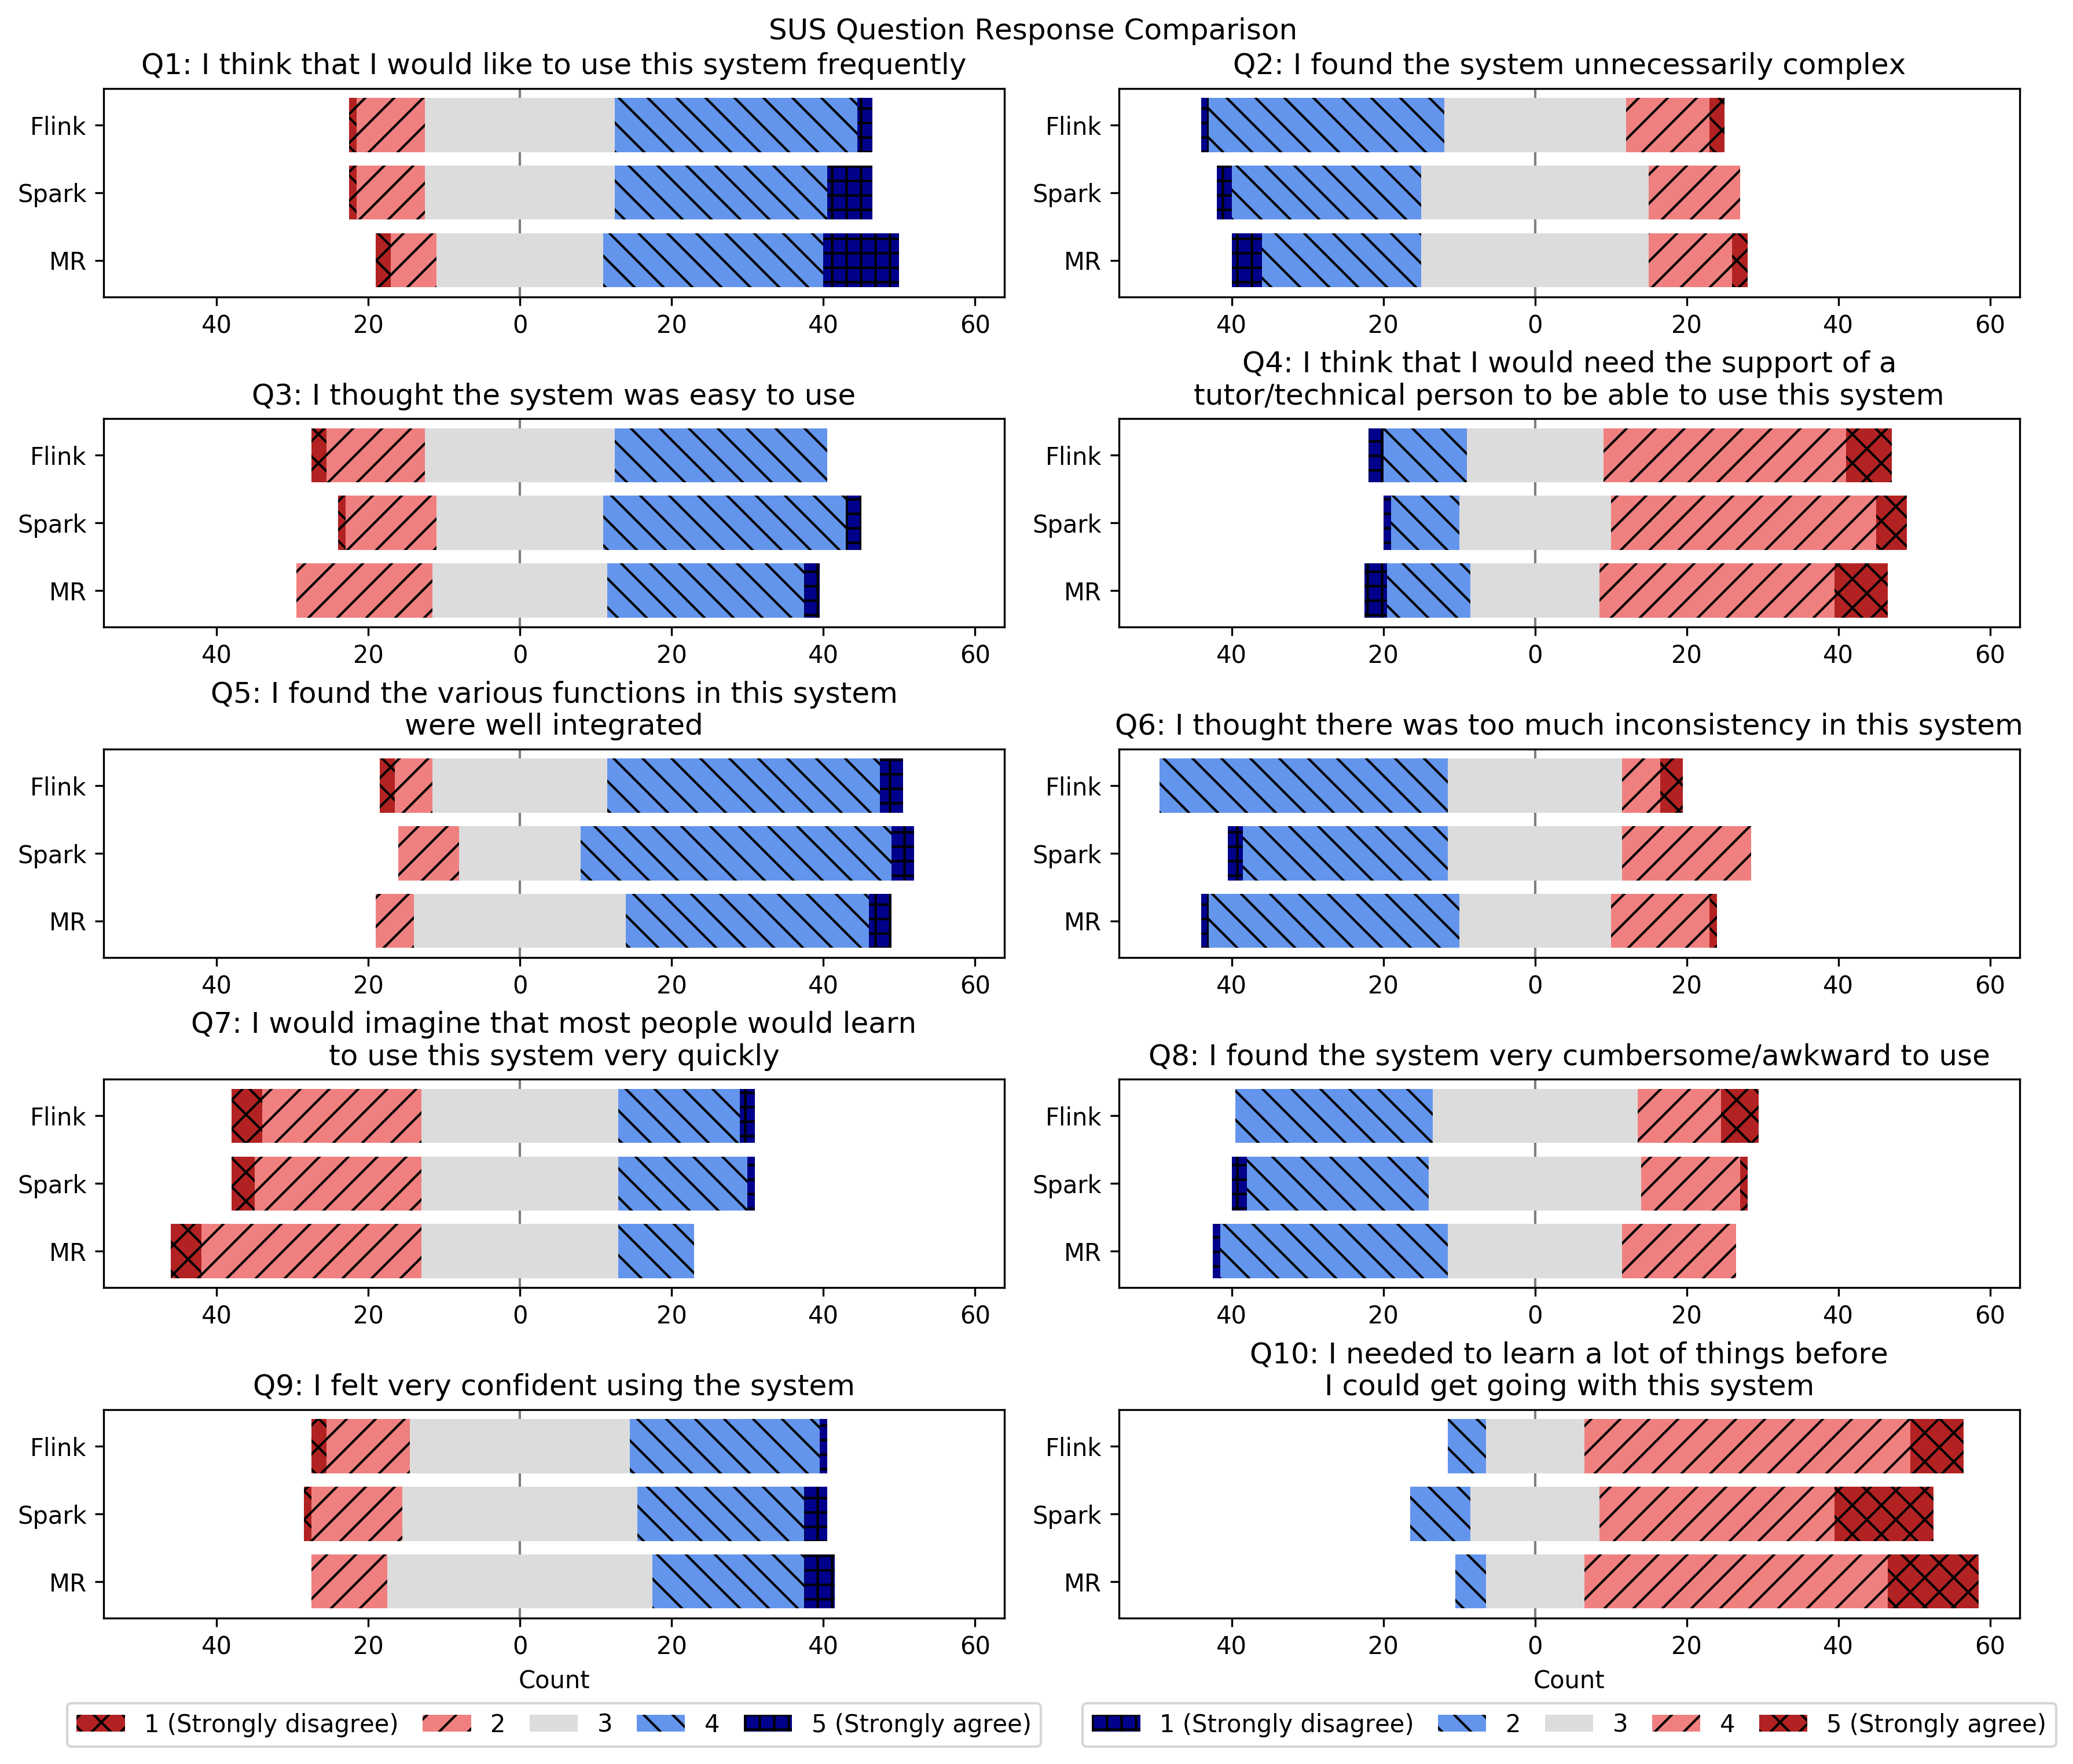
\includegraphics[width=6in]{./figs/sus-questions.png}}
    \caption{Diverging stacked bar charts \cite{HEIBERGER:DSBC:2014} displaying all 69 Likert scale responses for each SUS statement, however minus some missing individual responses. The five odd numbered statements on the left are `positively natured', such as ``Q3: I thought the system was easy to use'' -- agreeing with this statement is \emph{good} in terms of the system's usability. The five even numbered statements on the right are `negatively natured', such as ``Q2: I found the system unnecessarily complex'' -- agreeing with this statement is \emph{bad} in terms of the system's usability. To display this effectively, the legends on the left and right have their colours inverted -- blue is used to highlight good responses (regardless of a statements' positive/negative nature) and red for bad responses.}
    \label{SUS_QS}
  \end{figure}
  
  This subsection will discuss Figure~\ref{SUS_QS}, which displays all participants' responses to all ten SUS statements. The figure has been organised in a particular way considering the nature of the SUS. Its caption describes the intended interpretation.
  
  The first takeaway is that, for all ten questions, there is little difference in response distribution between the three systems. This explains why the SUS scores were very similar, as discussed in Section~\ref{PREF_SUS_SCORES}. It shows that in terms of usability as examined by the System Usability Scale, these three systems apparently share the same strengths and weaknesses, which is unintuitive considering that Apache Spark and Flink feature much higher level APIs.
  
  Furthermore, most questions had a good response as either a slight or strong majority -- a good sign for the usability of these systems. There are three exceptions: ``Q4: I think that I would need the support of a tutor/technical person to be able to use this system'', which most participants agreed with; ``Q7: I would imagine that most people would learn to use this system very quickly'', which a slight majority of participants disagreed with; and ``Q10: I needed to learn a lot of things before I could get going with this system'', which participants overwhelmingly agreed or strongly agreed with.
  
  These three questions with bad responses cover the topics of learning and support, and are the only questions in the set of ten concerning them. The other seven questions with good responses covered topics such as ease of use and system design and complexity. Is it normal that participants perceived the systems to be well designed, non-complex and usable, and yet hard to learn and in need of support to be used? One interpretation of this result is that participants felt that the systems were to be complex by design, considering their function as distributed computing engines, and in that context perceived them to be usable and such.
  
  However, the steep learning curve still needed to be addressed for them to use the system. We believe this is indicative of a prominent barrier to adoption of data science systems -- although they effectively abstract various distributed computing and dataflow challenges away, without simplifying the process of learning to use and overcoming difficulties with these systems, users with non-computing backgrounds will have significant trouble adopting them. From our experience and from the feedback of participants, we found the key areas for improvement to be first-party documentation and the process of debugging programs.


\subsection{Free-text Feedback and Other Impressions}
  
  Considering the participants' free-text feedback, and the experiences of instructors throughout execution of the study and teaching of its materials, we are able to highlight several areas of potential future improvement of the evaluated systems:
  
  \begin{itemize}
    \item Debugging in MapReduce was particularly difficult.
    \item MapReduce code tended to be overly verbose.
    \item Flink development environment setup was troublesome.
    \item Python support in Flink 1.2 felt immature.
    \item Spark and Flink felt quite similar to work with.
    \item Spark and Flink documentation covered basic usage quite well, but was limited for non-standard operations. Consequently, both Spark and Flink involved significant trial and error.
    \item Spark community support was good, but first-party documentation was lacking. Flink was described inversely.
  \end{itemize}
  
  We note that these points represent anecdotal observations only, but believe they are a good indicator of the general struggles faced by new users of these systems. Considering them, we would recommend that developers of these newer dataflow engines work to excel in regards to the on-boarding experience, the process of debugging, and the documentation of these systems -- especially for non-standard operations, perhaps by providing a very wide range of examples as opposed to focusing on canonical ones. Work in these suggested areas would complement the already greatly improved usability that  these systems provide, giving new users a streamlined experience of adoption, which is especially beneficial for individuals from non-distributed computing backgrounds.
\chapter{Comparison and Methodology}
\label{COMPARISON}

  Performing a comparison of multiple technologies, considering multiple factors, and having to communicate the results to users of differing technical backgrounds, is a challenge. Consideration needs to be taken in reducing biases between technologies. The chosen factors need to be of interest to the target audience. The communication method needs to be suitable for readers who want to know the technical details of the comparison, but also for those who may not be able to understand that detail and need a more distilled presentation. There are plenty more needs to consider, and this is why some methodology or theoretical framework is necessary before engaging in a comparison.

  However, we were unable to find any existing methodologies or frameworks to employ in our comparison, or even to apply principles or techniques from in the development of a new methodology. Thus we present an initial proposal of a multidimensional software comparison methodology to provide structure in considering all of these needs. The methodology provides guidance in the setup, execution and display of results for comparisons, in a way that is suitable for comparisons in different contexts, and intended for different audiences. In this sense it is not a very controlling or specific methodology, as that would largely restrict its applicability. Instead it seeks to guide the decision making process that occurs before commencing these comparisons, with the purpose of increasing comparison reliability and usefulness for the target audience.

  The following section will describe the proposed methodology and justify its design. The results section following that will apply the proposed methodology in performing a multidimensional comparison of Apache Hadoop MapReduce, Apache Spark and Apache Flink, considering each system's performance, usability and practicality.


\section{Methodology}

  We will describe the methodology, as introduced at the beginning of the chapter, in two parts. First, we provide an outline of the methodology, setting it out as a series of steps and touching on its intended outcomes for the readers of resulting comparisons -- useful as a quick reference during usage. This will be followed by an explanation of the design of the methodology and our justification of each step.


\subsection{Outline}

  \begin{figure}[ht]
      \begin{floatrow}
          \ffigbox
              {
                  \caption{\textbf{(Example)} Kiviat diagram for a system \textcolor{orange}{Z}}
                  \label{EX_KIV}
              }
              {
                  \begin{tikzpicture}[scale=.5,rotate=30]
                      \tkzKiviatDiagram[lattice=5]{Performance,Usability,Practicality}
                      \tkzKiviatLine[thick,color=orange,fill=orange,opacity=0.25](4.5,2,3.5)
                  \end{tikzpicture}

                  \textbf{(Example)} Larger measurements are better. See Table~\ref{EX_COMP_TBL} for more details.
              }
          \ffigbox
              {
                  \caption{\textbf{(Example)} Kiviat diagram comparing \textcolor{Green}{X}, \textcolor{blue}{Y} and \textcolor{orange}{Z}}
                  \label{EX_KIV_OVERLAY}
              }
              {
                  \begin{tikzpicture}[scale=.5,rotate=30]
                      \tkzKiviatDiagram[lattice=5]{Performance,Usability,Practicality}
                      \tkzKiviatLine[thick,color=Green,fill=Green,opacity=0.25](3,3,2)
                      \tkzKiviatLine[thick,color=blue,fill=blue,opacity=0.25](4.5,2,3.5)
                      \tkzKiviatLine[thick,color=orange,fill=orange,opacity=0.25](2.5,5,4.5)
                  \end{tikzpicture}

                  \textbf{(Example)} Larger measurements are better. See Figures~A, B and C for individual plots, and Table~\ref{EX_COMP_TBL} for more details.
              }
      \end{floatrow}
  \end{figure}

  \begin{table}[ht]
    \centering

    \caption{\textbf{(Example)} Comparison measurements for systems \textcolor{Green}{X}, \textcolor{blue}{Y} and \textcolor{orange}{Z}}
    \label{EX_COMP_TBL}

    \makebox[\textwidth]{\begin{threeparttable}
      \begin{tabular}{l r | l l l}
        \toprule
                              & \textbf{Weight} & \textbf{\textcolor{Green}{System X}} & \textbf{\textcolor{blue}{System Y}} & \textbf{\textcolor{orange}{System Z}} \\
        \midrule
        \textbf{Performance}  &                 &                                      &                                     &                                       \\
        Speed                 & 100\%           & \textbf{0.6}                         & \textbf{0.9}                        & \textbf{0.5}                          \\
        \midrule
        \textbf{Usability}    &                 & \textbf{0.6}                         & \textbf{0.4}                        & \textbf{1}                            \\
        Community answers     & 10\%            & 0.4                                  & 1                                   & 1                                     \\ 
        Complexity            & 30\%            & 0.8                                  & 0.2                                 & 1                                     \\ 
        Documentation         & 20\%            & 1                                    & 0.5                                 & 1                                     \\ 
        Examples              & 20\%            & 0.6                                  & 0.7                                 & 1                                     \\ 
        \midrule
        \textbf{Practicality} &                 & \textbf{0.4}                         & \textbf{0.7}                        & \textbf{0.9}                          \\
        License type          & 40\%            & 1                                    & 1                                   & 1                                     \\ 
        Shared environment    & 20\%            & 0                                    & 0.5                                 & 1                                     \\ 
        Security settings     & 40\%            & 0                                    & 0.5                                 & 0.75                                  \\ 
        \bottomrule
      \end{tabular}
      \begin{tablenotes}
        \item \textbf{(Example)} Higher values are better. Weightings have been provided as sensible defaults. You can adjust them better consider your circumstances.
        \source Direct the reader to the section of text which describes these measurements in detail, including how they were measured and normalised.
      \end{tablenotes}
    \end{threeparttable}}
  \end{table}
  
  This methodology guides the conception and display of results for multidimensional software comparisons. It requires the definition of an intended audience and context, as it emphasises the need to consider them throughout the design of the comparison and display of its results. The methodology aims to improve the structure and reliability of applied comparisons and their results.

  \begin{enumerate}
    \item Select a context and audience.
    \begin{itemize}
      \item For instance: a comparison of databases, with an audience of database researchers. This audience typically would be interested in different (more technical) considerations than an audience of, say, application developers.
    \end{itemize}

    \item Identify the key, high-level considerations for that context and audience.
    \begin{itemize}
      \item For instance: read throughput; write throughput; scalability; and fault tolerance.
      \item A less technical audience, say an application developer, may have less specific considerations: performance (as a whole); usability (the ease of learning the concepts and usage of a system, and becoming proficient with it); and practicality (the ease of a system's adoption into existing clusters, development environments and workflows).
    \end{itemize}

    \item Break down the identified considerations into one or more weighted, objective, normalised (to range from 0 to 1) measurements that are important to the audience.
    \begin{itemize}
      \item Explain each measurement and why it's being measured as part of its higher-level consideration.
      \item Explain the exact method of measurement and normalisation.
      \item Decide on each measurement's weighting as a percentage of its consideration's overall value, and explain the decisions.
    \end{itemize}

    \item Do your best to identify potential biases for these measurements and take steps to avoid them. Then perform the measurements.

    \item Present the results in three `tiers':
    \begin{enumerate}
      \item A set of Kiviat diagrams, also known as radar charts, comparing the values of the high-level considerations (cf. Figure~\ref{EX_KIV}), as a sum of their weighted measurements. Optionally, a combined Kiviat diagram overlaying each system (cf. Figure~\ref{EX_KIV_OVERLAY}) can \emph{additionally} -- not exclusively -- be presented. The combined Kiviat diagram should not be presented exclusively to avoid dependence on colour for interpretation, as this may not always be available to the reader.
      \item A table breaking down each high-level consideration into their individual measurements and weightings (cf. Table~\ref{EX_COMP_TBL}).
      \item A section of text describing each measurement in technical detail, including how their values were derived. The explanations from step 3 should be included here, as well as any details of steps taken to reduce potential biases.
    \end{enumerate}
  \end{enumerate}

  \begin{itemize}
    \item The intention here is that readers would start with the Kiviat diagrams for an overview, requiring less technical depth and understanding (relatively), but quickly covering what you identified to be their primary considerations.
    \item For more information they can resort to the table, which breaks down the derived values into their individual measurements and weightings.
    \item If unsure about any particular measurements or in search of more detail, they can resort to the full, technical descriptions provided.
    \item Additionally, readers are free to adjust the provided weightings based on the importance of each measurement given the their individual circumstance.
  \end{itemize}


\subsection{Design and Justification}
\label{DESIGN_AND_JUSTIFICATION}

  We realised that when it came to the design of a comparison methodology, it would be easy to fall into a trap where the methodology is too specific, such that it would primarily be useful for our research and other very similar comparisons -- say of other distributed computing engines -- only. In that sense we would not really be proposing a methodology at all, but just developing one for usage in our current research.

  However, we believe that while the situation described throughout this thesis -- data scientists lacking clear, reliable comparisons to support their selection of a distributed computing engine -- is indeed one which could benefit by these comparisons, there are undoubtedly many other contexts would be better off had it a stream of regular system comparisons. So, instead of focusing only on our context, we decided to try and provide guidance in the performance of multidimensional system comparisons to researchers looking to go down that path in other contexts too, as we experienced first-hand how little guidance already exists.

  System comparisons tend to be very specific though. Distributed systems need to consider fault tolerance and scalability, for instance, while the concept does not exist in programming languages on their own. A comparison of image compression libraries would consider the file size of the output images as one of its key metrics. Video streaming analysis systems would need to consider not only throughput, but also result latency. The list goes on, and we are using it to illustrate the challenge in developing a methodology that can be useful in all these contexts.

  It is for this reason that the methodology itself is rather high-level. It tries to guide the decision making process of the researchers who are conducting the comparison, such to help them avoid pitfalls that could damage the integrity of their comparison factors -- such as not empathising with the audience of the comparison (which we almost fell into ourselves) -- while still providing them the power necessary to tailor the comparison to the needs of their chosen systems and audiences.

  With different contexts in mind, another major theme we thought the methodology must consider is the differing audiences, and their level of contextual understanding, that can and should be considered when performing a comparison. As described in Chapter~\ref{INTRODUCTION} Section~\ref{STUDY_CONCEPTION}, we started off with the intention of performing this multidimensional comparison for a bioinformatics context, but considered what we thought to be important in that comparison instead of the needs that bioinformaticians themselves would consider. Having a computer science background myself, and a supervisor with extensive knowledge in databases and distributed systems, one might think that our interpretation of what a distributed system comparison needs to consider may be more ``authoritative'', and that the bioinformaticians considerations are somehow ``wrong''. However, we do not believe this to be the case. Instead it is us who must empathise with the changing needs of different audiences. Perhaps one system is more ``cutting edge'' or technically impressive, and while that may excite researchers in a related field, it could be largely irrelevant to data scientists or bioinformaticians who are looking for systems that they could use, given their less specialised technical knowledge, to increase the potential of their domain specific algorithms.

  Thus the two major themes coming into the design of this methodology were its applicability in a variety of technical contexts, and the consideration of a specific audience and their needs when performing a comparison. With this as a foundation, we attempt to explain and justify each step from the outline:

  \begin{description}
    \item[Step 1: Select a context and audience]
      We place this at the forefront because it should be in the researcher's mind as they are making all of their decisions regarding the comparison. The comparison is for a specific context and audience, and if that is forgotten then the usefulness or applicability of the comparison is in danger.
      
      The context can be as specific or as general as the researcher thinks is useful for that audience. In our case, a general context such as ``distributed data analysis tasks'' is sufficient, but for more technical audiences that would likely be too vague.
      
      Application of the methodology should be repeated and reconsidered even just for different audiences, to ensure their differing needs are being met, but of course measurements can be reused if present in both.

    \item[Step 2: Identify high-level considerations]
      The high-level considerations will each be assigned a value that can be compared between systems. A good rule of thumb in deciding on these high-level considerations is: if you asked a member of your audience what they think is important given a certain circumstance, without going into significant detail, what would they say? For instance, if you asked an application developer what they thought was important in comparing database engines, they might say performance; ease of use; and whether or not it could connect to their given application stack off the shelf. On the other hand, if you asked a database researcher the same question, they would likely refer to more technical considerations such as read/write throughput; scalability; and fault tolerance. Try talking to members of your intended audience to find out what they consider to be important -- you may be surprised.
      
      We label these considerations ``high-level'' because they are often not clearly measurements in themselves -- like usability or performance -- but are still an important consideration for a given audience. Just as these are ideally some of the first things to come to the reader's mind when they think of comparing the systems, we want them to be the first result they see in the comparison, providing a quick and useful high-level view of each system.
      
      By keeping these considerations and their values seperate instead of providing one overall value for each system, readers can judge the importance of each consideration given their individual circumstance. For instance, one user may be willing to put in significantly more effort to attain maximum performance, and thus values performance more greatly than usability, whereas others may be the opposite. If the values were compressed into one then this judgement would be harder to make.

    \item[Step 3: Break down considerations]
      Considerations should be broken down into measurements that are clearly related, and include an explanation where that relation is not immediately obvious. 

      They should also be as objective as possible. In our case, recognising that usability is an inherently subjective measure, we opted to perform a large-scale usability study and use an aggregated measurement of the participants' preferences.

      The measurements must then be normalised from 0 to 1 by some measure. Discrete measurements can simply have values assigned -- for instance, open source means 1, free community edition means 0.5, proprietary means 0 -- but be sure to justify any employed normalisation strategy.

      Finally, for considerations which have been broken down into multiple measurements, you must consider the weighting of each measurement. Note that this is simply a `default' weighting, as readers are encouraged to adjust the weightings to their individual circumstance, however it is important to provide sensible defaults considering that not all readers will do this. Again, you should provide justification for provided weightings.

      This arrangement provides readers with traceability and understanding, where sought after, and additionally flexibility in that they can adjust the weightings as they require. By exposing the thought processes behind these measurements, it hopefully also serves to increase the integrity of the comparison. It is important to be clear and objective to avoid a common concern in comparisons: that they are performed with a goal of skewing its results towards a particular system. Readers that may be suspicious should be able to read and understand how your measurements are being performed in a manner that indeed does not have this problem.

    \item[Step 4: Identify biases and perform measurements]
      Some measurements may be susceptible to biases in the process of being measured, so it is important to consider these potential biases prior to commencing measurements. There is not much guidance that can be provided here as it is very specific to the individual measurements, but as an example we identified a potential marking bias in our usability measurement -- where biases in the marking process could skew analysis results -- and while we attempted to reduce this bias, we ultimately ended up removing assignment marks from the analysis to be careful. If we had not taken the time to think of it as a potential bias, then it indeed could have ended up skewing the analysis results.

    \item[Step 5: Present the results in three tiers]
      We introduce the concept of `tiers' in terms of displaying the comparison results with the goal of assisting the reader in both navigating the multiple dimensions of results, and comprehending them. Three tiers are employed here, which grow more complicated from the `top' tier to the `bottom' tier. Each tier should be clearly linked for readers who seek more information on particular parts of the comparison. Definitions of the three tiers follows.
    
      The bottom tier is the most verbose, intended to provide the full story on how the considerations and measurements were decided upon and executed in a reliable manner. It should be a section of text that is referenced by the other tiers. All explanations and justifications from the previous methodology steps should be included here, and enough technical detail should be provided to clarify any potential misunderstandings or misinterpretations of your comparison. This tier may not be suitable for readers with more a shallow technical understanding, but that is ok -- they will have access to the other two tiers and can request further assistance if required. It is suggested that this section includes a breakdown of all measurements, their definitions and method of normalisation.

      Above this verbose textual tier, you should provide a table of measurements and their weightings, with Table~\ref{EX_COMP_TBL} acting as an example. The table's purpose is to quick provide a breakdown of the high-level considerations, for instance showing performance as a combination of throughput and scalability, and to separate the considerations' values into individual measurements and weightings. This provides slightly more technical detail than the high-level considerations, and should direct the reader to the section of text describing the measurements in full detail. It should also highlight that the weightings have been provided as `defaults', and recommend that the reader adjust them to their individual needs. This arrangement provides readers with a good level of flexibility without requiring significant technical knowledge or a large investment of time, but also the ability to dig in deeper if they require.
      
      Finally, at the top tier lies a visual overview of the systems comparison results, based on their high-level considerations. We suggest using Kiviat diagrams, also known as radar charts, as they can provide a clear and concise display of the multidimensional comparisons, with Figure~\ref{EX_KIV} as an example. The diagrams should refer to the table of measurements for further details.
      
      We recommend presenting the systems' diagrams in close proximity to support easy visual comparison. To this end, you could also present multiple systems in a single diagram, as shown in Figure~\ref{EX_KIV_OVERLAY}. However, it is important that this is not the only displayed chart as, if it is displayed depending on colour to separate each system, there may be accessibility issues for readers suffering from vision impairment. Thus, if you choose to include such a diagram with multiple systems overlayed and identified by colour, be sure to provide it in a complementary manner, referring to the individual diagrams which do not depend on colour, as we have done in Figure~\ref{EX_KIV_OVERLAY}.

      Note that Kiviat diagrams require a minimum of three dimensions (or variables), so a different choice of visualisation would be necessary in two-dimensional comparisons -- perhaps a bar chart.
  \end{description}

  With all of this in place, readers would be able to easily navigate the multidimensional comparison, starting from a concise, high-level visual representation, with directions to focus on the details that are important to them and easily being able to dig deeper to learn more. Naturally, the level of technical understanding required will increase as they descend the tiers of detail. A simple mechanism is provided to give readers some flexibility in adjusting measurement weighting.

  Researchers performing comparisons will have a structured approach to devising their comparison, and hopefully have the intended context and audience in mind throughout the decision making process. Yet, the methodology doesn't take away the flexibility researchers need to produce compelling comparisons in their specific contexts.


\section{Result}

  In this section we apply the methodology that was previously defined to the comparison of Apache Hadoop MapReduce, Apache Spark, and Apache Flink, in comparing their performance, usability, and practicality for data science. We present the application of the methodology in the series of steps as per its definition, however with the breakdown of individual measurements (step~3) and comparison results (step~5) combined into one -- because the full description of measurements needs to be included in the bottom tier of the comparison results, as per the definition in Subsection~\ref{DESIGN_AND_JUSTIFICATION}.

  \subsection{Step 1: Context and audience}
  \label{AUDIENCE}

  The comparison will be evaluating the suitability of Apache Hadoop MapReduce; Apache Spark; and Apache Flink, in the context of general, large-scale, batch data science or data analysis tasks. It is important to remember that stream processing is not being compared here. We consider the audience to be data scientists or researchers from varying disciplines who need to perform such large-scale batch analyses, but are not equipped with a traditional computer science or distributed computing background.
  
  Often these users are not in direct control of their distributed computing or cluster environments, and may be forced to utilise whatever communication layers have been made available to them from their institution or organisation -- perhaps Hadoop YARN or Apache Mesos. If a system is not compatible with said communication layers, then it could be too costly (perhaps in time) for the organisation to update the cluster to support it, and thus the system may not be a practical choice for this user's work.

  We observe that data scientists commonly have moderate to high experience with scripting or scientific programming languages such as Python or R, which are common tools in many scientific disciplines. While they may range from little or no to plenty of experience in distributed computing, they usually do not hold a deep understanding of the underlying concepts, because attaining a working knowledge of the systems is more often relevant to them than studying distributed computing principles.

  While these descriptions of the audience are speculative in nature, they represent our understanding of the problems faced by data scientists based on our observations and interactions with members of such communities, which we want to be particularly mindful of. Of course not everybody will face the same challenges, however we are trying to highlight that these users usually will often not possess the technical ability, understanding or the power to make technical changes, of an individual with a computer science or distributed computing background, and that we will be considering this throughout the comparison.

  \subsection{Step 2: High-level considerations}

  \begin{description}
    \item[Performance]
      This is essential given the context of large-scale data science or data analysis. Poor performance may rule out the applicability of a system for especially demanding experiments, where being an order of magnitude slower than another system could take computation time from hours to days, or days to weeks. Great performance, on the other hand, reduces incurred costs by improving resource utilisation and efficiency (noting that we are comparing the systems on the same underlying hardware), and also is able to facilitate performing more experiments in less time, increasing the potential of the research.

    \item[Usability] 
      A computer scientist or distributed computing specialist can be especially focused on the technical advantages of one system over another, for instance prioritising higher scalability or cutting edge performance -- they are often not concerned about the difficulty to learn or use the system, as with a deeper understanding of the underlying concepts, learning in such topics is something they are accustomed to.

      However, our audience of data scientists may struggle to learn and become proficient with more complex or verbose distributed computing engines -- it is a challenging topic, and a departure from their usual area of learning and research. While performance is undeniably important, this audience may be willing to sacrifice some of that in the interests of a system that they could learn to use more quickly, and thus work more effectively with.
      
      Systems with greater usability would support their users to focus more on their algorithms and analyses, rather than struggling to understand or implement a solution, or debug a problem. This difference may be worth significantly more to some users than, say, a 10\% performance boost on a less usable system. With that being said, we recognise that not all users have the same priorities, and the clear separation of usability and performance in this comparison will allow the individual reader to easily make a decision that suits their needs and preferences.

    \item[Practicality]
      Another problem we described our audience was likely to have was the limited control over their technical environment. They may not have the know-how, or even the permissions necessary to implement cluster or development environment changes, as may be necessary with different programming languages or cluster managers. This is why we consider practicality, which tries to capture the likelihood that a given dataflow engine will work without a requiring a user to change their development practices or environment.

      For instance, in an institution or organisation which provides an Mesos cluster to its data scientists, a request to install an additional custom resource negotiator such to use a particular distributed computing engine may be refused, deeming the system `impractical' in this case, compared to one which happens to support Mesos out of the box. In a similar situation, an organisation may already have a wide range of useful modules installed across a cluster for the Python programming language, which its practitioners may have become accustomed to using. Being required to deviate from established workflows could be difficult for many users.
  \end{description}
  
  These three high-level considerations are clearly separate, and provide what we believe to be a good coverage of potential measurements for comparison, in the sense that all the useful measurements we have been able to think of clearly fall beneath one of these three.

  \subsection{Steps 3 \& 5: Breakdown and results}
  \label{BREAKDOWN}

  \begin{figure}[p]
      \begin{floatrow}
          \ffigbox
              {
                  \caption{Kiviat diagram comparing the high-level consideration values of \textcolor{blue}{Apache Hadoop MapReduce}, \textcolor{orange}{Apache Spark} and \textcolor{Green}{Apache Flink}}
                  \label{COMP_KIV_OVERLAY}
              }
              {
                  \begin{tikzpicture}[scale=.5,rotate=30]
                      \tkzKiviatDiagram[lattice=5]{Performance,Usability,Practicality}
                      \tkzKiviatLine[thick,color=blue,fill=blue,opacity=0.25](2.258,0.875,3.75)
                      \tkzKiviatLine[thick,color=Green,fill=Green,opacity=0.25](3.835,4.415,3.25)
                      \tkzKiviatLine[thick,color=orange,fill=orange,opacity=0.25](3.818,4.67,3.5)
                  \end{tikzpicture}

                  Larger measurements are better. Performance measurements derived using data from \citeauthor{VEIGA:EVALUATION:2015} \cite{VEIGA:EVALUATION:2015}. See Figures~\ref{COMP_KIV_MR}, \ref{COMP_KIV_SPARK} and \ref{COMP_KIV_FLINK} for individual plots, and Table~\ref{COMP_TBL} for more details. If it looks like there are only two systems in the above diagram, that is because Apache Spark and Apache Flink are very close to overlapping in all considerations.
              }
          \ffigbox
              {
                  \caption{Kiviat diagram showing the high-level consideration values for \textcolor{blue}{Apache Hadoop MapReduce}}
                  \label{COMP_KIV_MR}
              }
              {
                  \begin{tikzpicture}[scale=.5,rotate=30]
                      \tkzKiviatDiagram[lattice=5]{Performance,Usability,Practicality}
                      \tkzKiviatLine[thick,color=blue,fill=blue,opacity=0.25](2.258,0.875,3.75)
                  \end{tikzpicture}

                  Larger measurements are better. Performance measurement derived using data from \citeauthor{VEIGA:EVALUATION:2015} \cite{VEIGA:EVALUATION:2015}. See Table~\ref{COMP_TBL} for more details.
              }
      \end{floatrow}
  \end{figure}

  \begin{figure}[p]
      \begin{floatrow}
          \ffigbox
              {
                  \caption{Kiviat diagram showing the high-level consideration values for \textcolor{orange}{Apache Spark}}
                  \label{COMP_KIV_SPARK}
              }
              {
                  \begin{tikzpicture}[scale=.5,rotate=30]
                      \tkzKiviatDiagram[lattice=5]{Performance,Usability,Practicality}
                      \tkzKiviatLine[thick,color=orange,fill=orange,opacity=0.25](3.818,4.67,3.5)
                  \end{tikzpicture}

                  Larger measurements are better. Performance measurement derived using data from \citeauthor{VEIGA:EVALUATION:2015} \cite{VEIGA:EVALUATION:2015}. See Table~\ref{COMP_TBL} for more details.
              }
          \ffigbox
              {
                  \caption{Kiviat diagram showing the high-level consideration values for \textcolor{Green}{Apache Flink}}
                  \label{COMP_KIV_FLINK}
              }
              {
                  \begin{tikzpicture}[scale=.5,rotate=30]
                      \tkzKiviatDiagram[lattice=5]{Performance,Usability,Practicality}
                      \tkzKiviatLine[thick,color=Green,fill=Green,opacity=0.25](3.835,4.415,3.25)
                  \end{tikzpicture}

                  Larger measurements are better. Performance measurement derived using data from \citeauthor{VEIGA:EVALUATION:2015} \cite{VEIGA:EVALUATION:2015}. See Table~\ref{COMP_TBL} for more details.
              }
      \end{floatrow}
  \end{figure}

  \begin{table}[p]
    \centering

    \caption{Comparison high-level considerations and their measurements for systems \textcolor{blue}{Apache Hadoop MapReduce}, \textcolor{orange}{Apache Spark} and \textcolor{Green}{Apache Flink}}
    \label{COMP_TBL}

    \makebox[\textwidth]{\begin{threeparttable}
      \footnotesize
      \begin{tabular}{l r | l l l}
        \toprule
        & \textbf{Weight}
        & \textbf{\textcolor{blue}{Apache Hadoop MapReduce}}
        & \textbf{\textcolor{orange}{Apache Spark}}
        & \textbf{\textcolor{Green}{Apache Flink}} \\
        \midrule
        \textbf{Performance}       &      & \textbf{0.451}  & \textbf{0.764}  & \textbf{0.767} \\
        Speed                      & 50\% & 0.215           & 0.883           & 0.695          \\ 
        Scalability                & 50\% & 0.688           & 0.644           & 0.838          \\ 
        \midrule
        \textbf{Usability}         &      & \textbf{0.175}  & \textbf{0.934}  & \textbf{0.883} \\
        From usability study       & 70\% & 0.25            & 0.905           & 1              \\ 
        REPL availability          & 10\% & 0               & 1               & 0.5            \\ 
        Specialised APIs           & 20\% & 0               & 1               & 0.667          \\ 
        \midrule
        \textbf{Practicality}      &      & \textbf{0.75}   & \textbf{0.7}    & \textbf{0.65}  \\
        Programming languages      & 50\% & 1               & 0.4             & 0.3            \\ 
        Cluster/deployment options & 50\% & 0.5             & 1               & 1              \\ 
        \bottomrule
      \end{tabular}
      \normalsize
      \begin{tablenotes}
        \item Higher values are better. Weightings have been provided as sensible defaults. You can adjust them better consider your circumstances.
        \source Performance values derived using data from \citeauthor{VEIGA:EVALUATION:2015} \cite{VEIGA:EVALUATION:2015}. Each of these measurements are elaborated under Subsection~\ref{BREAKDOWN}.
      \end{tablenotes}
    \end{threeparttable}}
  \end{table}

  \begin{table}[p]
    \centering

    \caption{Performance: Raw data}
    \label{RAW_PERFORMANCE_DATA}

    \makebox[\textwidth]{\begin{threeparttable}
      \scriptsize
      \begin{tabular}{l r | l l l}
        \toprule
        && \multicolumn{3}{c}{Execution time (seconds)} \\
        Task & Cluster size
        & \textbf{\textcolor{blue}{Apache Hadoop MapReduce}}
        & \textbf{\textcolor{orange}{Apache Spark}}
        & \textbf{\textcolor{Green}{Apache Flink}} \\
        \midrule
        WordCount
        & 13 & 483.21 & 136.25 & 326.68   \\
        & 25 & 244.96 & 64.39  & 183.32   \\
        & 37 & 171.54 & 58.86  & 138.24   \\
        & 49 & 131.21 & 56.71  & 114.27   \\[1ex]
        Grep                              
        & 13 & 1737.32 & 32.39 & 45.18    \\
        & 25 & 1671.03 & 35.86 & 41.89    \\
        & 37 & 1139.02 & 36.96 & 45.38    \\
        & 49 & 878.31  & 39.48 & 48.21    \\[1ex]
        TeraSort                          
		& 13 & 838.12 & 449.83 & 467.77   \\
        & 25 & 339.07 & 139.35 & 186.06   \\
        & 37 & 202.64 & 100.17 & 106.75   \\
        & 49 & 119.53 & 85.70  & 76.68    \\[1ex]
        Connected Components
		& 13 & 1414.46 & 242.44 & 301.07  \\
        & 25 & 1081.13 & 184.82 & 162.09  \\
        & 37 & 855.96  & 135.64 & 138.68  \\
        & 49 & 759.12  & 114.95 & 110.81  \\[1ex]
		PageRank
		& 13 & 1716.19 & 944.07 & 280.85  \\
        & 25 & 1106.48 & 593.74 & 177.83  \\
        & 37 & 905.71  & 398.71 & 134.68  \\
        & 49 & 773.73  & 287.98 & 112.79  \\[1ex]
		$k$-means
		& 13 & 2501.97 & 309.50 & 1204.38 \\
        & 25 & 1705.36 & 225.47 & 652.33  \\
        & 37 & 1377.72 & 177.12 & 501.45  \\
        & 49 & 1373.56 & 182.62 & 396.95  \\
        \bottomrule
      \end{tabular}
      \normalsize
      \begin{tablenotes}
        \source \citeauthor{VEIGA:EVALUATION:2015} \cite{VEIGA:EVALUATION:2015} responded to our request for the numbers pertaining to Figure~1 in their performance comparison paper -- shown in this table.
      \end{tablenotes}
    \end{threeparttable}}
  \end{table}

  \begin{table}[p]
    \centering

    \caption{Performance: Task execution time comparison}
    \label{COMP_SPEED_TBL}

    \makebox[\textwidth]{\begin{threeparttable}
      \footnotesize
      \begin{tabular}{l | r l r l r l}
        \toprule
        & \multicolumn{6}{c}{Execution time with 13 nodes (seconds), and normalised value\tnotex{COMP_SPEED_TBL:A}} \\
        Task
        & \multicolumn{2}{l}{\textbf{\textcolor{blue}{Apache Hadoop MapReduce}}}
        & \multicolumn{2}{l}{\textbf{\textcolor{orange}{Apache Spark}}}
        & \multicolumn{2}{l}{\textbf{\textcolor{Green}{Apache Flink}}} \\
        \midrule
        WordCount            & 483.21   & 0.28 & 136.25 & 1    & 326.68   & 0.42 \\ 
        Grep                 & 1,737.32 & 0.02 & 32.39  & 1    & 45.18    & 0.72 \\ 
        TeraSort             & 838.12   & 0.54 & 449.83 & 1    & 467.77   & 0.96 \\ 
        Connected Components & 1,414.46 & 0.17 & 242.44 & 1    & 301.07   & 0.81 \\ 
        PageRank             & 1,716.19 & 0.16 & 944.07 & 0.30 & 280.85   & 1    \\ 
        $k$-means            & 2,501.97 & 0.12 & 309.50 & 1    & 1,204.38 & 0.26 \\[1ex]
        \textbf{Average}     && \textbf{0.215} && \textbf{0.883} && \textbf{0.695} \\
        \bottomrule
      \end{tabular}
      \normalsize
      \begin{tablenotes}
        \item[a] \label{COMP_SPEED_TBL:A} Higher values are better. The normalised value is the lowest execution time across the task divided by the system's individual execution time for that task.
    \source Execution speeds from \citeauthor{VEIGA:EVALUATION:2015} \cite{VEIGA:EVALUATION:2015}, as visible in Table~\ref{RAW_PERFORMANCE_DATA}. This measurement is elaborated in Subsection~\ref{BREAKDOWN} under ``Performance -- Speed''.
      \end{tablenotes}
    \end{threeparttable}}
  \end{table}

  \begin{table}[p]
    \centering

    \caption{Performance: Task execution scalability comparison}
    \label{COMP_SCALABILITY_TBL}

    \makebox[\textwidth]{\begin{threeparttable}
      \footnotesize
      \begin{tabular}{l | r l r l r l}
        \toprule
        & \multicolumn{6}{c}{Execution speedup from 13 to 49 nodes, and normalised value\tnotex{COMP_SCALABILITY_TBL:A}} \\
        Task
        & \multicolumn{2}{l}{\textbf{\textcolor{blue}{Apache Hadoop MapReduce}}}
        & \multicolumn{2}{l}{\textbf{\textcolor{orange}{Apache Spark}}}
        & \multicolumn{2}{l}{\textbf{\textcolor{Green}{Apache Flink}}} \\
        \midrule
        WordCount            & 268\% & 1    & 140\% & 0.52  & 186\% & 0.69  \\ 
        Grep                 & 98\%  & 1    & -18\% & -0.18 & -6\%  & -0.06 \\ 
        TeraSort             & 601\% & 1    & 425\% & 0.71  & 510\% & 0.85  \\ 
        Connected Components & 86\%  & 0.50 & 111\% & 0.65  & 172\% & 1     \\ 
        PageRank             & 122\% & 0.54 & 228\% & 1     & 149\% & 0.65  \\ 
        $k$-means            & 82\%  & 0.40 & 69\%  & 0.34  & 203\% & 1     \\[1ex]
        \textbf{Average}\tnotex{COMP_SCALABILITY_TBL:B} && \textbf{0.688} && \textbf{0.644} && \textbf{0.838} \\
        \bottomrule
      \end{tabular}
      \normalsize
      \begin{tablenotes}
        \item[a] \label{COMP_SCALABILITY_TBL:A} Higher values are better. The normalised value is the system's individual speedup for the task divided by the maximum speedup across that task.
        \item[b] \label{COMP_SCALABILITY_TBL:B} The Grep task was not included in calculating this average, as described in Subsection~\ref{BREAKDOWN} under ``Performance -- Scalability''.
        \source Speedup derived using execution speeds from \citeauthor{VEIGA:EVALUATION:2015} \cite{VEIGA:EVALUATION:2015}, as visible in Table~\ref{RAW_PERFORMANCE_DATA}. This measurement is elaborated in Subsection~\ref{BREAKDOWN} under ``Performance -- Scalability''.
      \end{tablenotes}
    \end{threeparttable}}
  \end{table}

  An overview of the comparison results, quickly comparing the value for each consideration, is presented in Figure~\ref{COMP_KIV_OVERLAY}. An overview of the individual measurements and how they contribute to their considerations' values is presented in Table~\ref{COMP_TBL}.

  What follows is the elaboration of each measurement, including how they were decided, measured and normalised.

  The stable versions at the time of conducting measurement were: Apache Hadoop MapReduce v2.9.0; Apache Spark v2.2.1; Apache Flink v1.4.1. The performance measurements, which utilised external research, were performed with versions: Apache Hadoop MapReduce v2.7.2; Apache Spark v1.6.1; and Apache Flink v1.0.1. The usability study was performed with versions: Apache Hadoop MapReduce v2.7.2; Apache Spark v2.1.1; Apache Spark v1.2.1 -- the stable versions at the time.

  \begin{description}
    \item[Performance -- Speed (50\%)]
      \textit{Summary (based on data from \citeauthor{VEIGA:EVALUATION:2015} \cite{VEIGA:EVALUATION:2015}):} How does the execution speed of each system, given a set of 6 tasks in a consistent environment, compare to the other systems? Apache Hadoop MapReduce: 0.215; Apache Spark: 0.883; Apache Flink: 0.695. Higher values represent lower execution times. The tasks included in the comparison are WordCount, Grep, TeraSort, Connected Components, PageRank and $k$-means -- the latter three of which are iterative algorithms. \medskip

      \textit{Details:} During literature review we found a rich collection of research evaluating the performance of distributed computing engines. Considering this, we have decided to incorporate research by \citeauthor{VEIGA:EVALUATION:2015} \cite{VEIGA:EVALUATION:2015}, which compares all three of the subject systems reliably. As discussed in Chapter~\ref{LITERATURE_REVIEW} Subsection~\ref{SYSTEM_COMPARISONS}, there is little benefit to be found in repeating similar studies over utilising this quality, existing evaluation. Please refer to that paper for full performance evaluation details, especially including Section~IV of the paper, where the hardware and software configuration used in the experiments is described -- different configurations would provide different comparison results.

      For the purpose of measurement, we contacted the author of the paper requesting the data behind what had been presented in Figure~1 of the performance comparison -- as the figure did not show the exact numbers, only bars for comparison. The author kindly provided the data, which we display in Table~\ref{RAW_PERFORMANCE_DATA}.

      For each of the six compared tasks, using the measurement at the lowest (13) node configuration, the system with the lowest execution time is assigned a value of 1, and the other systems' a value inversely proportional to that -- so a system that took double the time to complete the task would have a value of 0.5. This also serves to normalise the values. The final value used for this measurement is each of the systems' average across the six normalised values.

      This approach is has been chosen considering that systems may be strong at certain tasks, but weak at others, so picking a single task for comparison is inappropriate. Taking the average of the tasks' values is approximate, as it may be the case that a particular user will value the performance of a given task more often than some other, however we cannot be sure of each reader's priorities and so will not attempt to provide weight to these tasks ourselves -- readers can apply individual weightings to the tasks if they know that a particular one is more important to them. Furthermore, the lowest (13) node configuration is examined as opposed to those with more machines in an attempt to minimise the effect of improved scalability and instead focus on more direct system performance. Scalability is covered in a separate measurement, immediately below.

      Table~\ref{COMP_SPEED_TBL} presents the execution times for each task, and the average.

    \item[Performance -- Scalability (50\%)]
      \textit{Summary (based on data from \citeauthor{VEIGA:EVALUATION:2015} \cite{VEIGA:EVALUATION:2015}):} How does the speedup of each system compare, given a set of 5 tasks, as the size of the cluster increases from 13 nodes to 49 nodes? Apache Hadoop MapReduce: 0.688; Apache Spark: 0.644; Apache Flink: 0.838. Higher values represent greater speedups. The tasks included in the comparison are WordCount, TeraSort, Connected Components, PageRank and $k$-means -- the latter three of which are iterative algorithms. \medskip

      \textit{Details:} During literature review we found a rich collection of research evaluating the performance of distributed computing engines. Considering this, we have decided to incorporate research by \citeauthor{VEIGA:EVALUATION:2015} \cite{VEIGA:EVALUATION:2015}, which compares all three of the subject systems reliably. As discussed in Chapter~\ref{LITERATURE_REVIEW} Subsection~\ref{SYSTEM_COMPARISONS}, there is little benefit to be found in repeating similar studies over utilising this quality, existing evaluation. Please refer to that paper for full performance evaluation details, especially including Section~IV of the paper, where the hardware and software configuration used in the experiments is described -- different configurations would provide different comparison results.
      
      We use the same dataset as in the speed comparison, Figure~1 in the performance comparison paper (presented in Table~\ref{RAW_PERFORMANCE_DATA} here), in performing this measurement, however this time looking at the speedup from the minimal 13 node cluster to the maximal 49 node cluster. This limits the applicability of our measurement to a context where cluster growth is from 13 to 49 nodes -- please bear this in mind, as the results may not be applicable if your situation involves the usage of substantially more nodes.

      Specifically, for each system and each of the six compared tasks, the `speedup' is the execution time at the minimal 13 nodes divided by the execution time at the maximal 49 nodes, minus 1, displayed as a percentage. The final value for this measurement was intended to be the systems' average across all six tasks. However, the Grep task was completed very quickly by both Spark and Flink even at the smallest cluster size, resulting in a slowdown as the scale increased and additional overheads were imposed unnecessarily. We believe that in this particular case, the scalability of the systems is not accurately represented, and thus will exclude it -- the Grep task -- from the final calculation.

      Table~\ref{COMP_SCALABILITY_TBL} presents the speedup for each task, and the average excluding Grep.

    \item[Usability -- From usability study (70\%)]
      \textit{Summary:} This value is based on how many participants from our usability study prefer to use a given system, considering the entire participant pool (rather than the Java-only pool from Chapter~\ref{USABILITY_STUDY} Subsection~\ref{LANGUAGE_INFLUENCE}). Apache Hadoop MapReduce: 0.25; Apache Spark: 0.905; Apache Flink: 1. Higher values represent a higher proportion of reported preferences.\medskip

      \textit{Details:} The usability study performed and detailed in Chapter~\ref{USABILITY_STUDY} compared multiple usability factors between the subject systems -- primarily: reported system preference, System Usability Scale (SUS) values, and reported time spent. However, we decided this measurement would only consider reported system preference, for various reasons specific to this usability study's execution:

      \begin{enumerate}
        \item Our intention was to use the SUS score as a usability value, as that is the purpose of the survey. However, our usage of the SUS was experimental -- as described in Chapter~\ref{USABILITY_STUDY} Subsection~\ref{SUS} -- and, we believe, ultimately unsucessful. Specifically, the three systems turned out very similar in all measures related to the SUS, as explored in Chapter~\ref{USABILITY_STUDY} Subsections~\ref{PREF_SUS_SCORES} and~\ref{SUS_INDIV}. Technically, this could mean the three systems indeed are similar in usability, but we find this unlikely considering the very large difference in preference when looking at Apache Hadoop MapReduce, and also our personal experiences with the systems. Thus due to a lack of understanding, we choose not to rely on SUS data in this comparison.
        \item Discluding the SUS, we were left with the reported system preferences and time spent working on the assignments. Unfortunately, a mishap in the collection of assignment~1 time spent data, as described in Chapter~\ref{USABILITY_STUDY} Subsection~\ref{EXEC_SURVEYS}, prevented us from being able to reliably compare the three systems' with that data. Although we may have come to the same decision to not use this data even if it had been appropriate, as the reported system preference could be considered more relevant.
      \end{enumerate}

      Thus, to utilise the performed large-scale usability study, we are left with reported system preferences as our means of comparison. Here we must decide which participant pool to consider: the full pool, or the Java-only pool. This decision is necessary considering the lack of Python support for Apache Flink in our usability study, as described in Chapter~\ref{USABILITY_STUDY} Section~\ref{EXECUTION}, which could have introduced biases to the experiment. The analyses in Chapter~\ref{USABILITY_STUDY} Subsection~\ref{LANGUAGE_INFLUENCE} found that all of our initial conclusions remained consistent in the Java-only pool, indicating that little bias was introduced. The only exception here was in the reported system preferences, which changed notably, and understandably -- Python users may have felt disappointed by the fact that they could use Apache Spark with Python, but not Flink, and this could have affected their reported preference. However, this would have had no effect on Java users.

      Our audience for this comparison is data scientists, and in that sense it would be wrong to exclude Python users from the pool, as Python is a very common tool among data scientists and for general purpose data analytics. Including the Python users would mean that any of the aforementioned biases will be represented in the comparison results here. However, trying to exclude them could be considered inaccurate, as they were resultant of Flink's immature Python support at the time, as opposed to some error in the design or execution of the usability study. Thus, we will be considering the reported preference from the full pool of participants.

      Therefore, a system's value is simply the percentage of participants who preferred that system, as reported in Chapter~\ref{USABILITY_STUDY} Subsection~\ref{PREF_SUS_SCORES}, divided by the percentage of the most preferred system for normalisation.

    \item[Usability -- REPL availability (10\%)]
      \textit{Summary:} This represents whether or not each system provides first-party REPL (Read-Eval-Print Loop) support. Apache Hadoop MapReduce: 0; Apache Spark: 1; Apache Flink: 0.5.\medskip

      \textit{Details:} We believe being able to utilise a REPL environment is very useful when writing and debugging distributed programs. It assists in debugging and understanding the workings of a program, by being able to interactively inspect the data at its various steps through the distributed computation -- a graph of operations in Spark and Flink. It can help users become proficient with a system faster than had it not been available.

      REPL availability is linked to whether the programming language itself includes a REPL, and whether or not a first-party connector has been provided, as it is non-trivial to connect the language's standard REPL environment to a cluster for the given system.
      
      Looking at Hadoop MapReduce, abitrary programming languages are supported via Hadoop Streaming, which utilises arbitrary executables, but this does not mean that there is REPL support. Hadoop's APIs are only available in Java which does not include REPL support, and we find no indication of any other first-party mechanism. Thus its value is 0.
      
      Spark and Flink provide APIs in Scala and Python (and R for Spark), all of which are languages with REPL support. Spark provides connectors for all three of these languages, giving it a value of 1 for this measurement. Flink provides a connector for Scala -- one of its two applicable languages, giving it a value of 0.5 for this measurement.

    \item[Usability -- Specialised APIs (20\%)]
      \textit{Summary:} How many first-party specialised API packages or libraries are provided for each system, compared to the other systems? Apache Hadoop MapReduce: 0; Apache Spark: 1; Apache Flink: 0.667.\medskip

      \textit{Details:} Spark and Flink provide higher-level, specialised APIs for certain use cases, for instance including graph computation and machine learning. Such APIs are very useful for practitioners performing related work, reducing the need for low-level learning and often improving execution speed and performance with thanks to their specialised implementations. Note that here we are focused on batch computing, so streaming libraries will not be considered.

      Working without such APIs can be difficult -- I for one am not sure how I would go about graph computation in Spark or Flink without using their higher-level APIs. This difficulty would be exaggerated for our audience, who likely have more limited technical ability compared to a distributed computing specialist or computer scientist.

      MapReduce does not appear to have any such high-level APIs itself. Sometimes it is the foundation of higher-level systems or frameworks which may compile down to it, such as Apache Pig or Apache Hive, however we do not consider those in this measurement, as the user is not actually using MapReduce in these cases. In contrast, users can interchange between the standard \texttt{DataSet}, SQL, and the Gelly graph processing APIs easily, within the same Flink program. Considering this, MapReduce has a value of 0 for this measurement.

      Interestingly, both Spark and Flink provide: a higher level SQL API to enable SQL-like querying over relational data, however still in beta in Flink; a machine learning library (MLlib for Spark and FlinkML for Flink); and a graph processing library (GraphX for Spark and Gelly for Flink). As the SQL API is still in beta for Flink, it will not be considered in this measurement. Thus Spark achieves a value of 1, and Flink a value one-third lower, considering that its beta SQL API is not being included: 0.667.

    \item[Practicality -- Programming languages (50\%)]
      \textit{Summary:} How many programming languages have first-party support in all of each systems' core APIs? Apache Hadoop MapReduce: 1; Apache Spark: 0.4; Apache Flink: 0.3.\medskip

      \textit{Details:} This measurement is appropriate considering our definition of practicality, the ease of a system's adoption into existing clusters, development environments and workflows. This could be especially relevant to our audience, as described in Subsection~\ref{AUDIENCE}.

      MapReduce includes a feature named Hadoop Streaming, which facilitates the usage of arbitrary executables to act as mappers, reducers and combiners. Through this mechanism, any programming language installed on the cluster can be used. Fine-tuning implementations by customising partitioners or comparators, for instance, must still be done via Java, however often the majority of work will be completed in the mapper, reducer and driver, and so Hadoop Streaming provides a great level of flexibility here. In that sense, its value for this measurement is 1, as it supports artbitrary programming languages.

      Since MapReduce supports arbitrary languages, the values for the other systems cannot be relative to MapReduce. But then what should they be relative to? We can make an estimate that if 10 languages were supported, then it is very likely that there will exist at least one language in which a given user will be familiar with. Thus supporting 10 languages, for the purpose of assigning values for this measurement, is equivelant to supporting an arbitrary number of languages like MapReduce. Therefore each supported language adds 0.1 to the measurement's value, up to a maximum of 1. We realise that this is not quite a precise method of measurement, however it should suffice in providing an approximate value here, for the lack of a better techinque.

      Spark's core batch processing APIs can be considered as the `classic' RDD API, as well as the `modernised' \texttt{DataFrame} and \texttt{DataSet} APIs. All of these APIs are supported in the Scala, Java, Python and R programming languages. Accordingly, Spark has a value of 0.4 for this measurement.

      Flink's core batch processing API is the \texttt{DataSet} API, which provides support to the Scala, Java and Python programming languages, thus earning a value of 0.3 for this measurement. While feature parity across these three languages is not complete (which is not at all unexpected), it is quite significantly behind for Python. Although we experienced significant difficulty working with the Python API in Flink v1.2.1, we are unaware of its state now, in v1.4.1. Python users should especially consider performing some exercises with the system before deciding to commit to it.

    \item[Practicality -- Cluster/deployment options (50\%)]
      \textit{Summary:} How does the number of first-party supported cluster deployment options compare between each system? Apache Hadoop MapReduce: 0.5; Apache Spark: 1; Apache Flink: 1.\medskip

      \textit{Details:} We consider this measurement as our audience will often not be in direct control of their cluster environment, perhaps having to request cluster changes from their institution or organisation, which could be a time-consuming or, in the worst case, fruitless undertaking. Thus a system that provides support for more cluster configurations has a higher chance of being practical for a given user.

      We must consider the provider of a cluster deployment option for the purposes of this measurement: should we only consider clusters with first-party support, like how Spark itself provides Apache Mesos support (\texttt{new SparkConf().setMaster("mesos://HOST:5050")})? What about cases where the deployment target itself advertises support for the distributed computing engine, like how Mesos provides instructions on how to run MapReduce applications within (and not vice versa)? 

      Firstly, it is impractical to check `all' cluster deployment options to see if they provide support to the compared systems. Furthermore, it may be risky to do so, considering that the methods they provide may have fallen out of date -- it is not the cluster's obligation to provide support to specific distributed computing engines, but rather to provide interfaces for arbitrary systems to connect to.

      While it is also not the engine's obligation to provide support to the given clusters, it is more likely that if some cluster management software is being advertised in an engine's first-party documentation as a deployment option, that they will in fact maintain support for that -- bearing in mind that these are not experimental systems or deployment options; they are intended for usage in production environments. After all, cluster managers or resource negotiators like Mesos and YARN are purposefully `pluggable', in the sense that arbitrary systems can connect to it and request resources, whereas distributed computing engines are not.

      Thus we will only consider cluster deployment options with first-party support.

      How are standalone cluster configurations related to this measurement? Standalone deployment options make it significantly easier to use a system on one's local machine, perhaps for development or experimental purposes. On the other hand, they certainly will not be an existing cluster configuration that can be utilised without needing to directly modify or request modification to a user's cluster (unless the system is already being used), which means that these are not related to our definition of practicality. So we will not consider them in this measurement -- but note that all three of the compared systems are capable of executing locally, without a cluster manager installed. Spark and Flink also include standalone cluster managers which can be used instead of dedicated ones like Mesos or YARN.

      With all this in mind, we observe that MapReduce only supports YARN, while Spark and Flink support both YARN and Mesos. Thus this measurement's value is 0.5 for MapReduce, and 1 for Spark and Flink.

    \item[Practicality -- Software licensing (N/A)]
      We considered this to be a measure of practicality as incompatible software licensing could be prohibitive under some circumstances. However all three of the subject systems are top-level Apache projects, and thus feature identical licensing models, making the measurement useless in this particular case.
  \end{description}

  Looking again at Figure~\ref{COMP_KIV_OVERLAY}, we can see that in comparison to Apache Spark and Apache Flink, Apache Hadoop MapReduce is quite far behind in both performance and especially usability, but similar on the grounds of practicality -- with its support for arbitrary programming languages compensating for its lack of Apache Mesos deployment support.
  
  The three high-level considerations for Spark and Flink reached very similar values. Spark's performance was slightly superior in terms of speed, but inferior in scalability (in the scope of scaling from 13 to 49 nodes) compared to Flink. We recommended that readers explore the individual measurements and adjust their weightings to more closely match your individual requirements and preferences, which map help to differentiate between the two systems. However, even after doing this they may end up similar, as we found that they both included many of the same features and characteristics.

  We are very happy with the experience of using our proposed multidimensional comparison methodology. It provided a structured approach to devising, performing, and presenting the results of the comparison. Continued improvement of the methodology following further application in other contexts should see it grow to be an excellent tool in future software comparisons.
\chapter{Conclusion}

  We observed that Apache Hadoop MapReduce \cite{HADOOP:HOMEPAGE} remained a dominant choice for distributed computing in the bioinformatics field -- and likely in other scientific disciplines -- in comparison to the newer, more dataflow oriented Apache Spark \cite{SPARK:HOMEPAGE,ZahariaCFSS:HotCloud10} and Apache Flink \cite{FLINK:HOMEPAGE,CarboneKEMHT:DEBU2015}. Our impression was that in these disciplines where practitioners are not generally equipped with deep distribution computing knowledge, it is difficult to keep up with the rapid pace of innovation in dataflow engines, especially where there exists a lack of academic guidance in matters other than performance. While performance is indeed always a concern, we argue that it is less so within fields where users of these distributed systems are not distributed computing experts themselves. Other concerns including usability, which we define as the ease of learning to use and becoming proficient with a system, and practicality, which we define as the flexibility of a system in terms of adopting or fitting it into one's existing development environment and workflow, become very important for users who do not have the ability to learn complex distributed computing topics on a whim, or configure clusters or computing environments as they please.
  
  Thus our research firstly investigated this hypothesis -- that Hadoop MapReduce was indeed a dominant choice in bioinformatics and other scientific disciplines, over newer, more performant and dataflow oriented systems. With that validated, we proceeded to both confirm that these newer systems are indeed more suitable for problem solving in these sub-disciplines, and then to explore potential solutions that could increase adoption of these newer systems in consideration of that. Effectively, we have bridged the gap which we identified as missing non-performance related comparisons between these engines, in the hope that this information will provide guidance to practitioners in said disciplines, granting them the confidence to work with the systems most suitable for them, rather than resorting to MapReduce by default -- ultimately helping the disciplines to reap the benefits of the unending innovations of the distributed computing field.
  
  In summary, to achieve these goals we:
  
  \begin{itemize}
    \item Performed a thorough literature review, and created a web scraper to analyse a large number of bioinformatics related research -- thus validating our hypothesis that this problem in fact existed.
    \item Performed a novel large-scale usability study to confirm that Apache Spark and Apache Flink were indeed more suitable for distributed computing tasks within scientific disciplines like bioinformatics. This doubled up as a large part of the multidimensional software comparison that was developed.
    \item Proposed a methodology for developing multidimensional software comparisons (considering the lack of an already well-developed one). The output comparisons are intended to facilitate effective communication of a wide range of considerations, and provide the individual reader the ability to conveniently navigate and even appropriate the comparison results based on their specific use case.
    \item Applied this proposed methodology, along with usability data from the large-scale usability study, performance data from \citeauthor{VEIGA:EVALUATION:2015} \cite{VEIGA:EVALUATION:2015}, and researched practicality data, to produce a multidimensional comparison of Hadoop MapReduce, Spark and Flink -- thus bridging the identified gap in knowledge.
  \end{itemize} \medskip
  

  In more detail, we implemented a web scraper that was used to scrape one year of data from the BMC Bioinformatics journal, which we combined with an analysis of papers from three years of more sparse bioinformatics research presented within the IEEE BigData conference. With this information we examined the systems being used in recent bioinformatics research, considering both purely bioinformatics perspectives (within the BMC Bioinformatics journal), as well as from a more distributed computing perspective but with bioinformatics applications (within the IEEE BigData conference). This practice was effective, successfully providing a holistic view of the technical landscape in the bioinformatics field (at least pertaining to distributed computing), and accordingly validating our hypothesis that newer dataflow engines were struggling to gain traction within the field. With more time, it could be valuable to negotiate with other representative journals which may not be open access like BMC Bioinformatics, to facilitate scraping of a wider range of data -- however even without doing so, we consider our findings quite reliable. \medskip
  

  We performed a large-scale usability study with students in a cloud computing class, which addressed the lack of usability data concerning modern distributed data processing platforms, and act as the dominant part of the usability consideration in our multidimensional comparison. The usability study primarily involved survey data collected from three surveys -- one following completion of each of three data analysis assignments. The first assignment used MapReduce, and the latter two employed a crossed A/B test with Spark and Flink. To the best of our knowledge, this usability study was the first of its kind, and so substantial effort was placed into ensuring its reliability and making it a quality contribution to this research.
  
  The usability study worked well: study participation was high; students cooperated in the crossed A/B test with perhaps surprisingly little organisational difficulty; only a small portion of survey data was left unfilled; and student course satisfaction levels remained high (data not shown). Catering for the diversity of a class with both IT and data science students is a challenge, and we see the learned lessons and careful design of our study as one of our contributions.
  
  We found that participants' perceived preferences were strongly in favour of either Spark or Flink in comparison to MapReduce, however there was little difference between the two modern systems themselves. There was also no significant difference in the amount of time participants reported they required to complete the assignments using either of the modern systems. Thus from a usability point of view and without a more specific use case in mind, both Spark and Flink seem to be equally suitable choices over MapReduce, most likely due to the high-level nature of these data processing platforms.
  
  In performing our usability study, we experimented with using the System Usability Scale (SUS) \cite{BROOKE:SUS:1996} to measure and compare the usability of the three systems, which we have not seen used in programming contexts despite being found effective elsewhere \cite{BANGOR:SUS_EVALUATION:2008}. However despite its convenience, we ultimately did not find it highly effective, as it did not provide much insight into the usability of each system, nor did it correlate with perceived preferences. Looking in detail at responses to individual SUS questions highlighted weaknesses in the learn-ability and need for support in all three systems, supporting what we believe to be key areas for improvement in data science systems which would greatly support their adoption by users with non-computing backgrounds: first-party documentation and the process of debugging programs.
  
  A further finding when performing the usability study was that participants preferred the first of the data processing engines that they encountered in the class -- either Spark or Flink. Interestingly, there was also a significant difference in SUS scores between the assignments, however there was no suitable data to highlight the cause of this difference. We suspect that it is a combination of a first-used advantage and differences in assignment difficulty.
  
  However, Python with Flink was not working to an acceptable degree and we thus could not provide support and learning resources for them. We recognise that this would have introduced some bias to the study, and to account for this analyses were repeated with Python user data excluded, where it became apparent that among Java users Flink was more often reported as preferred than Spark. A subsection of the usability study's analysis was dedicated to examining these potentially introduced biases, where we found that all of our initial conclusions remained consistent in the Java-only pool, indicating that little bias was introduced.
  
  Overall, we consider the usability study a success in that we could measure meaningful differences between big data processing systems in their usability, which might contribute to their adoption as much as technical aspects or raw performance -- especially considering that all of them scale well when adding more virtual machines. There were indeed some challenges faced during execution of the study, leading us to advise allowing a generous amount of time for preparation, and if at all possible to avoid having to continue preparation after the usability study's commencement -- but that was the nature of our situation and we believe we executed it well, all things considered. With experience, we now hold the opinion that the medium of university classes is an excellent one for performing software comparisons, and recommend other researchers to consider doing the same if that is indeed an option. \medskip
  
  
  We then continued to produce a clear, reliable comparison of these three systems, helping to highlight the strengths and weaknesses of each, and guiding practitioners in making informed decisions regarding the system that would best fit a given project. The comparison did not solely consider the context of bioinformatics, but of data science and distributed data analysis in general, because this phenomenon is likely not limited to the single scientific field.

  The comparison was multidimensional because performance is not the only factor necessary to consider when deciding which system to use -- as is especially the case for less technical audiences, such as data scientists, who may struggle to adopt cutting edge systems substantially more than, say, a computer scientist or distributed computing researcher. The need grows further considering the compared software, wherein by their nature, all distributed systems will be able to scale and achieve immense speeds by adding more virtual machines; so it would take more than only performance to differentiate or decide between these systems.
  
  On a larger scale, the presence of regular, high quality multidimensional comparisons would improve the pace of innovation in scientific fields, which are not naturally focused on keeping up with the cutting edge of the software they may be using. Thus this particular comparison is useful now, considering the lack of related research, but needs to be kept relevant with more comparisons that follow the ongoing developments of the distributed computing field.

  To facilitate both this research, and to promote and assist in the conduct of ongoing comparisons of software in general, we proposed a methodology for performing multidimensional software comparisons -- which we were unable to find an existing standard for. This research also features its first application: the comparison of MapReduce, Spark and Flink, in consideration of performance, usability and practicality for data science.

  The methodology was highly effective in this application, where it provided both guidance and structure in devising, performing, and displaying the multidimensional comparison results. Already a valuable contribution, we are excited to follow the growth of the methodology as it is applied in varying contexts. We found that it was indeed general enough to be applied to a variety of situations, while still providing useful guidance in how we could massage our collected data into a format navigable by readers with a variety of needs. We found that our choice of performance, usability and practicality as high-level considerations was effective, as all relevant metrics seemed to naturally fall into one of those three. If repeated, we would consider doing more case studies relating to the practicality consideration, perhaps by visiting actual researchers within relevant sub-disciplines, and learning what the prohibiting factors are in trying to adopt a new system in reality as opposed to anecdotally.

  The performed multidimensional comparison itself combined existing research from \citeauthor{VEIGA:EVALUATION:2015} \cite{VEIGA:EVALUATION:2015} for the performance consideration, with both our large-scale usability study and more simple static analyses for the usability and practicality considerations.
  
  The results align with our hypothesis that Spark and Flink are indeed superior to MapReduce both in terms of performance and usability -- in fact being significantly so. While MapReduce exhibited slightly improved scalability to Spark, its speed of execution was far behind the other systems. Owing to MapReduce's support of arbitrary programming languages, it scored similar to Spark and Flink in consideration of practicality.

  Spark and Flink turned out similar across all three considerations. With that being said, one of the proposed methodology's goals is to provide the output comparison's readers with the flexibility to adjust the weighting of involved measurements. We especially recommend doing so here, in the hopes of providing differentiation between the two systems to better suit the reader's individual circumstances. Notably, Spark exhibited superior performance in the form of speed, but inferior in the form of scalability, compared to Flink. We believe this comparison achieves our goal of empowering readers to understand the differences between these systems, not only in consideration of performance, and thus hopefully provide confidence in making the switch more appropriate systems where applicable. \medskip
  
  
  Overall we consider this research a success, as none of its hypotheses were invalidated, and all of its goals were reasonably met. It forms the first step by our group, and an early step in the field as a whole, to better understand the usability and adoption of big data processing systems for data science. Our long-term goal is to identify factors and to develop techniques for improving the usability and impact of the next generation of big data systems. The proposed methodology will hopefully grow and serve an even wider goal, of promoting ongoing execution of software comparisons. This is necessary to assist the many scientific disciplines, such as bioinformatics, in using the most appropriate software for their research, and thus increasing their pace of innovation.
\printbibliography[heading=bibintoc]


\end{document}